% % \part{机器学习与深度学习}
% % \chapter{深度学习}

% \documentclass[UTF8]{ctexbook}

% \ctexset{
%     part/number = \chinese{part}
% }
% \usepackage{multirow}
% \usepackage{amsmath}% ams 数学公式
% \usepackage{amsfonts}% ams 数学字体
% \usepackage{bbm}%重影字体
% \usepackage{amssymb,latexsym}% ams 数学符号与LaTeX数学符号
% \usepackage{mathrsfs}% 花式符号
% \usepackage{ntheorem}%定理、定义、证明
%     \theoremstyle{nonumberplain}
%     \theoremheaderfont{\bfseries}
%     \theorembodyfont{\normalfont}
%     \theoremsymbol{$\square$}
%     \newtheorem{Proof}{\hskip 2em 证明}
%     \newtheorem{theorem}{\hspace{2em}定理}[chapter]
%     \newtheorem{definition}{\hspace{2em}定义}[chapter] % 如果没有章, 只有节, 把上面的[chapter]改成[section]
%     \newtheorem{axiom}[definition]{\hspace{2em}公理}
%     \newtheorem{lemma}[definition]{\hspace{2em}引理}
%     \newtheorem{proposition}[definition]{\hspace{2em}命题}
%     \newtheorem{corollary}[definition]{\hspace{2em}推论}
%     \newtheorem{remark}{\hspace{2em}注}[chapter] %类似地定义其他“题头”. 这里“注”的编号与定义、定理等是分开的
%     \newtheorem{Assumption}{\hspace{2em}假设}[chapter]

% %算法伪代码
% %http://blog.csdn.net/lwb102063/article/details/53046265
% \usepackage{algorithm}
% \usepackage{algorithmicx}
% \usepackage{algpseudocode}
%     \floatname{algorithm}{算法}
%     \renewcommand{\algorithmicrequire}{\textbf{输入:}}
%     \renewcommand{\algorithmicensure}{\textbf{输出:}}
% % 罗马数字:示例:\rom{2}
% \makeatletter
% \newcommand*{\rom}[1]{\expandafter\@slowromancap\romannumeral #1@}
% \makeatother

% \usepackage{enumerate}%itemiz环境。\begin{enumerate}[step 1][a)]可以使用 A,a,I,i,1 作为可选项产生 \Alph,\alph,\Roman,\roman,\arabic 的效果
% \usepackage{cite}%参考文献
%     \bibliographystyle{plain}
% \usepackage{extarrows}% 带参数的箭头
% \usepackage{hyperref}% 超链接
% \usepackage{pifont}%然后在正文输入\ding{172}~\ding{211}得到相应数字,要是要①就输入:\ding{172}②就输:\ding{173}
% %\usepackage[CJKbookmarks, colorlinks, bookmarksnumbered=true,pdfstartview=FitH,linkcolor=black,citecolor=black]{hyperref}%超链接的格式设置
% \hypersetup{
%     colorlinks=false,% 去掉超链接颜色
%     pdfborder=0 0 0% 取消超链接的边框
% }
% \usepackage{graphicx}% 图片管理
% \usepackage{caption}
% \usepackage{subcaption}%并排的图各有标题
% \graphicspath{{images/}}% 设置图片搜索路径
% \usepackage{float,varwidth}% 浮动体
% \usepackage{booktabs}% 三线表
% \usepackage{fancyhdr}% 页眉设置
% \usepackage{xcolor}% 颜色宏包
% \usepackage{colortbl}% 彩色表格
% \usepackage{listings}% 代码高亮
% \usepackage{caption}% 对标题进行控制,如让\caption标题的字体缩小一号,同时数字标签使用粗体可以用:\usepackage[font=small,labelfont=bf]{caption}
% \usepackage{xfrac,upgreek}%分别是行间公式如a/b的形式(将原来的命令\frac改成\sfrac)和希腊字体的宏包的
% \usepackage{mathtools}%lgathered和rgathered环境把公式向左向右对齐
% \usepackage{tabularx}%提供自动延伸的表列,(X列格式说明符),文字过长时可以自动转行
% \usepackage{longtable}%长表格
% \usepackage{enumitem}%enumerate宏包的升级
% \usepackage{harpoon}%数学公式的矢量
% \usepackage{bookmark}%目录的书签
% \renewcommand{\headwidth}{\textwidth}%图片并排,这个要列在所有宏包的后面
% \definecolor{codegreen}{rgb}{0,0.6,0}
% \definecolor{codegray}{rgb}{0.5,0.5,0.5}
% \definecolor{codepurple}{rgb}{0.58,0,0.82}
% \definecolor{backcolour}{rgb}{0.95,0.95,0.92}
% \lstset{
%     commentstyle=\color{codegreen},
%     keywordstyle=\color{magenta},
%     numberstyle=\tiny\color{codegray},
%     stringstyle=\color{codepurple},
%     basicstyle=\footnotesize,
%     breakatwhitespace=false,% 断行只在空格处
%     breaklines=true,% 自动断行
%     captionpos=b,% 标题位置
%     keepspaces=true,
%     numbers=left,
%     numbersep=5pt,
%     showspaces=false,
%     showstringspaces=false,
%     showtabs=false,% 显示
%     tabsize=2% TAB 被当作两个空格
% }
% \topmargin=0pt\oddsidemargin=0pt\evensidemargin=0pt
% \textwidth=16.5cm\textheight=23cm\raggedbottom%我这么设置是为了缩小页边距,满足有的文字无法转行
% \pagestyle{headings}%页眉为章节标题,无页脚
% \setlength{\abovecaptionskip}{10pt}
% \setlength{\belowcaptionskip}{-15pt}%图片表格的前后距离设置
% \CTEXsetup[format={\zihao{-3}\raggedright\bfseries}]{section}%设置节的格式


% \begin{document}
% \part{机器学习与深度学习}
\chapter{深度学习}
\section{深度置信网络DBN}
    \par
    Hinton于2006年首次提出深度置信网络(deep belief network, DBN),从而引起了深度学习的热潮。之后,深度学习模型又发展出了深度玻尔兹曼机DBM、堆积自动编码器SAE、卷积神经网络CNN、用于语音和文本处理的RNN以及对抗生成网络GAN等等。在开发DBN之前,多层前向神经网络MLP往往只有3到4层的深度,太深的网络被认为是难以优化的,直到DBN出现后,在MNIST数据集上准确率超过(核)支持向量机,才使得深度网络开始得到认可。尽管DBN与其它深度网络相比,已经失去了研究者和工业开发者的青睐,我们还是应该标注一下,除了表示敬意之外,也可以由此开启深度学习之旅。顺带一提的是,深度学习工具有许多,并且它们的更新很快,所以后面大部分内容我们都只介绍深度模型的理论。同时,由于深度学习的发展速度很快,基本上是日新月异的,每天都有新成果、新应用,这使得我们想要全面学习它变得困难。我们不得不挑选一些具有里程碑意义的网络来进行介绍。
    \subsection{DBN网络结构}
        \par
        我们知道,限制玻尔兹曼机RBM是没有网络层次结构的,如果要将其分层,可以分为可视层$v$和隐含层$h$。基本的RBM网络结构如图(\ref{fig:RBM网络结构图})所示
            \begin{figure}[H]
            \centering
            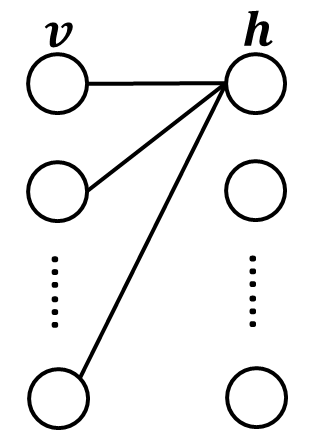
\includegraphics[height=3cm]{images/RBM_net_structure.jpg}
            \caption{RBM网络结构图}
            \label{fig:RBM网络结构图}
            \end{figure}
        % \textcolor[rgb]{1 0 0}{todo:图片:RBM网络结构图}\\
        形式上有$v,h$两层。现在,我们考虑能否把多个RBM网络“堆积”在一起?虽然多个BP网路“堆积”而成MLP不易于训练,但是多个RBM堆积未必不可以训练,因为RBM网络的训练方式并不是基于反向传播算法的。
        \par
        我们先来将2个RBM堆积在一起,如图(\ref{fig:2个RBM堆积图})所示,其中:第一个$RBM_{1}$和隐含层$h^1$是第二个$RBM_{2}$的可见层,其权重为$W^1,W^2$。
\begin{figure}[H]
  \centering
  \begin{varwidth}[t]{\textwidth}
    \vspace{0pt}
    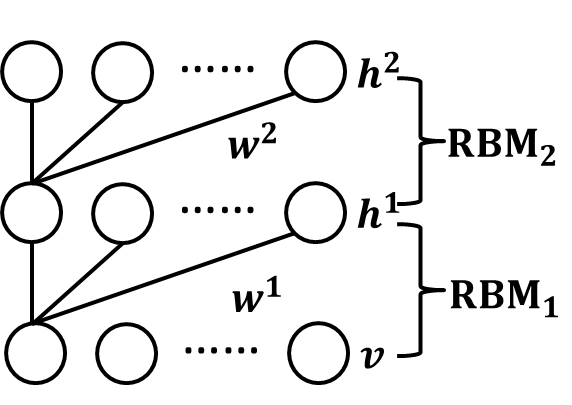
\includegraphics[height=3cm]{images/2RBM_accumulation1.jpg}
  \end{varwidth}
  \qquad\qquad
  \begin{varwidth}[t]{\textwidth}
    \vspace{0pt}
    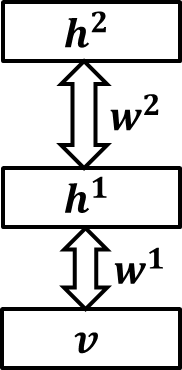
\includegraphics[height=3cm]{images/2RBM_accumulation2.jpg}
  \end{varwidth}
  \caption{2个RBM堆积图}
  \label{fig:2个RBM堆积图}
\end{figure}
        % \textcolor[rgb]{1 0 0}{todo:图片:2个RBM堆积图}\\
        图(\ref{fig:2个RBM堆积图})中的神经元连接方式是无向连接/双向连接的,并且不考虑阈值$b$。我们先训练$RBM_1$,当这个$RBM_1$收敛到数据集时,我们得到其权重$W^1$,并得到$RBM_1$的隐含层激活模式(样本/向量)。我们将每个隐含层激活模式作为数据集来训练第2个$RBM_2$。一个有趣的事情是:如果$v$中的神经元数目和$h^2$相等,那么我们训练完$RBM_2$得到$W^2$是$W^1$的转置,$RBM_2$可以是$h^1$的一个很好的模型。
        \par
        现在将底层$RBM_1$的权重改变一下,准确的说是将其连接方式改变一下,我们只保留$h^1\rightarrow v$方向上的权重,而不要$v\to h^1$方向的权重。这样,网络就变成了一个有向网络,如图(\ref{fig:2个RBM的右向网络图})(a)所示
\begin{figure}[H]
  \centering
  \begin{varwidth}[t]{\textwidth}
    \vspace{0pt}
    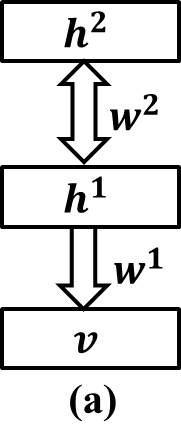
\includegraphics[height=4cm]{images/2RBM_right_net1.jpg}
  \end{varwidth}
  \qquad\qquad
  \begin{varwidth}[t]{\textwidth}
    \vspace{0pt}
    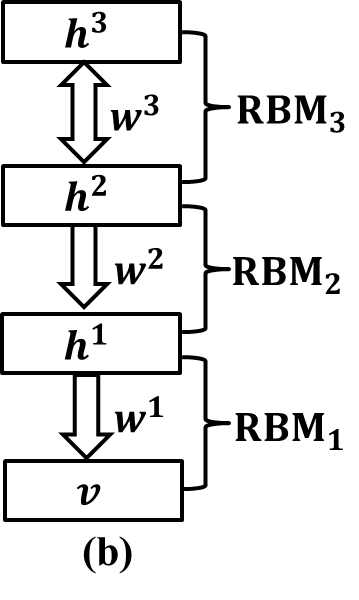
\includegraphics[height=4cm]{images/2RBM_right_net2.jpg}
  \end{varwidth}
  \caption{2个RBM的右向网络图}
  \label{fig:2个RBM的右向网络图}
\end{figure}
        % \textcolor[rgb]{1 0 0}{todo:图片:2个RBM的右向网络图}\\
        至于为什么这样做,以后有机会再讨论。我们将其扩展到4层,如图(\ref{fig:2个RBM的右向网络图})(b)所示,只有在顶部的$RBM_3$中是真的双向连接,而在$RBM_2,RBM_1$中,只有下行权重,所以网络也不再是RBM网络了。它更像logistics置信网络(1992.Neal),称这种由RBM和logistics置信网络混合的深度网络为深度置信网络DBN。
        \par
        下面,我们考虑如何运行DBN。以图(\ref{fig:2个RBM的右向网络图})(b)为示例,为了从这个模型中生成数据,或者说为了让这个模型来拟合样本的分布,首先,通过顶层$RBM _3$在$h^2,h^3$中进行热平衡采样,结束之后,就有了$h^2$。这里的$h^2$是$RBM_3$定义的$h^2$的先验分布,然后,将$h^2$通过权重$W^2$传递到$h^1$,无论$h^1$中得到什么样的二值状态,紧接着通过$W^1$传递给$v$,来得到生成数据。所以,我们执行一个从$h^2$开始自顶而下的传播,去得到其它各层的状态,就像在一个sigmoid置信网络中一样。
        \par
        现在,我们考虑一个深层的DBN,由$L$个RBM堆积而成,如图(\ref{fig:L层DBN示意图})所示
            \begin{figure}[H]
            \centering
            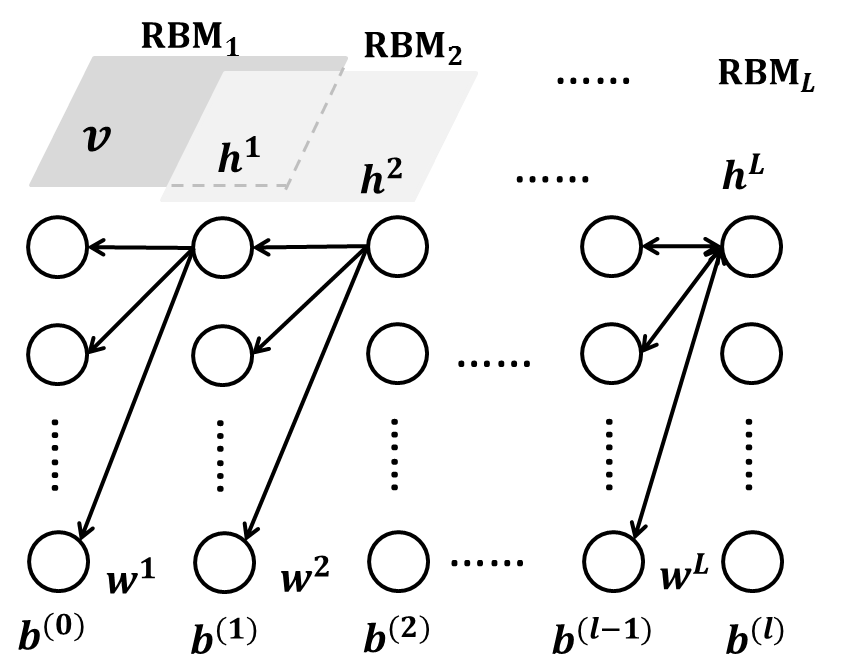
\includegraphics[height=4cm]{images/L_layer_DBN_illustration.jpg}
            \caption{L层DBN示意图}
            \label{fig:L层DBN示意图}
            \end{figure}
        % \textcolor[rgb]{1 0 0}{todo:图片:L层DBN示意图}\\
        图中共有$L$个RBM。整体来看,DBN有1个可视层$v$和$L$个隐含层$h^{(l)}(l=1,2,\dots,L)$,并且有$L$个权重矩阵$W^{(l)}(l=1,2,\dots,L)$,有$L+1$个阈值$b^{(l)}(l=0,1,\dots,L)$。其中:$b^{(0)}$是可视层$v$的偏置。 假设我们已经有了所有的权重$W = \{W^{(l)}\}$和阈值$b= \{b^{(l)}\}$,令$\theta\triangleq (W,b)$,于是有下面的概率公式
        \begin{align*}
        & p(h^{(L)},h^{(L-1)}) \propto \exp\left(b^{(L)}{}^\mathrm{T} h^{(L)} + b^{(L-1)}{}^\mathrm{T} h^{(l-1)} + h^{(L-1)}{}^\mathrm{T}W^{(L)}h^{(L)}\right)\\
        & p(h_i^{(l)}=1|h^{(l+1)}) = \sigma  \left( b_i^{(l)} + W_{\cdot i}^{(l+1)}{}^\mathrm{T}h^{(l+1)} \right)  \quad l=1,2,\dots,L-2\\
        & p(v_i = 1| h^{(1)}) = \sigma \left( b_i^{(0)}+W_{\cdot i}^{(1)}{}^\mathrm{T}h^{(1)} \right)
        \end{align*}
        \par
        如果$v$不是二值01,而是实值$v_i\in R$,可以用下式来是实现高斯RBM
        \begin{align*}
        v\sim N(v|b^{(0)}+ W^{(1)}{}^\mathrm{T}h^{(1)} ,\beta^-1)
        \end{align*}
        其中:$\beta$是协方差矩阵,是一个对角矩阵。这里我们不详细介绍高斯RBM。上面,我们说过从$h^3$开始,如何生成$v$,其联合概率分布为
        \begin{align*}
        p(v,h^1,h^2,\dots,h^L) = p(v|h^1)p(h^1|h^2)\cdots p(h^{L-2}|h^{L-1})p(h^{L-1}|h^{L})
        \end{align*}
        \par
        虽然是DBN,但是我们的目标仍然是求$\theta$使样本概率最大,即样本的似然函数最大。现在的问题是:样本$v$的概率是多少呢?

    \subsection{DBN学习算法}
        \par
        对于分类问题$x,y$,DBN的学习一般分为2个过程:
        \begin{enumerate}
        \item 使用无标签数据$x$(只用$x$,不用$y$)无监督的训练DBN。这里,关于无监督的训练DBN,可以采用2006.Hinton提出的贪心逐层算法,即对每一个RBM进行训练。在无监督训练DBN后,得到参数$\theta\triangleq (W,b)$。
        \item 使用有监督数据$x,y$进行$\theta$的微调。在无监督$\theta$的基础上,将$\theta$视为网络初始参数,将整个网络视为前向网络,用BP算法对网络权重$W$和阈值$b$进行微调。
        \end{enumerate}
        \par
        采用贪心逐层算法训练DBN是容易实现的,我们将DBN分为$L$个RBM,对每个RBM进行训练,并得到权重和阈值$W^{(l)},b^{(l)}$
        \begin{align*}
        & \mathbb{E} _{v\sim P_{data}} \log p(v)\\
        & \mathbb{ E}_{v\sim P_{data}} \mathbb{E}_{h^{(1)}\sim p^{(1)}(h^{(1)}|v)} \log p^{(2)}(h^{(2)})\\
        & \qquad \vdots
        \end{align*}
        其中:$p^{(1)}$是第一个RBM表示的的概率分布。在大多数应用中,对DBN进行贪心逐层训练后,需要再花费时间进行联合训练,训练好的DBN可以直接用于生成任务。如果要将其用于分类任务,我们可以将贪心算法求得的参数$\theta$作为网络参数的初始值,搭建如图(\ref{fig:DBN的权重微调网络})的多层前向神经网络MLP
            \begin{figure}[H]
            \centering
            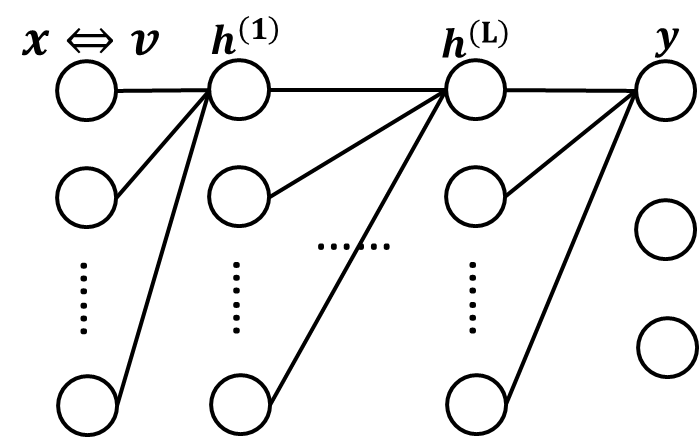
\includegraphics[height=3cm]{images/DBN_Weighted_Micro_Transformation_Net.jpg}
            \caption{DBN的权重微调网络}
            \label{fig:DBN的权重微调网络}
            \end{figure}
        % \textcolor[rgb]{1 0 0}{todo:图片:DBN的权重微调网络}\\
        并且
        \begin{align*}
        & h^{(1)} = \sigma \left( b^{(1)} + v^\mathrm{T}W^{(1)} \right) \\
        & h^{(l)} = \sigma \left( b_i^{(l)} + h^{(l+1)}{}^\mathrm{T} W^{(l)} \right) \quad l = 2,3,\dots,L
        \end{align*}
        然后,用BP等算法来对MLP 网络进行训练,微调其参数$\theta$。


\section{深度玻尔兹曼机DBM}
    \subsection{DBM网络结构}
        \par
        DBM(Deep Boltzmann Machine)是另一种深度\underline{生成模型},由Salakhutdinov和Hinton于2009年开发。与DBM不同的是,它是一个完全无向的网络。以一个含有两个隐含层的DBM为例,其网络结构示意图如图(\ref{fig:3层DBM网络结构示意图})所示
            \begin{figure}[H]
            \centering
            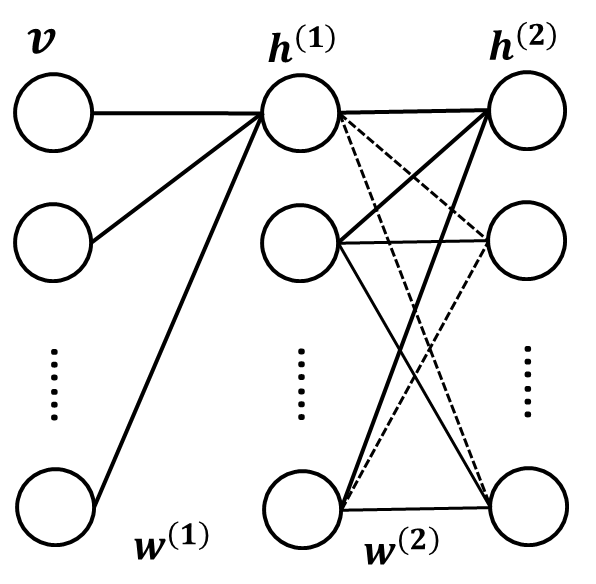
\includegraphics[height=4cm]{images/3DBM_net_structure.jpg}
            \caption{3层DBM网络结构示意图}
            \label{fig:3层DBM网络结构示意图}
            \end{figure}
        % \textcolor[rgb]{1 0 0}{todo:图片:3层DBM网络结构示意图}\\
        DBM是一个基于能量的模型,这意味这模型中变量(神经元)的联合概率分布可以由能量函数表示:在参数$\theta$给定下,网络的能量函数(忽略偏置$b$)为
        \begin{align*}
        E_\theta(v,h^{(1)},h^{(2)}) = -v^\mathrm{T}W^{(1)}h^{(1)} - h^{(1)}{}^\mathrm{T} W^{(2)}h^{(2)}
        \end{align*}
        由此,网络的联合概率分布(Boltzmann分布)为
        \begin{align*}
        p(v,h^{(1)},h^{(2)}) = \frac{1}{Z_\theta} \exp \left( -E_\theta(v,h^{(1)},h^{(2)}) \right)
        \end{align*}
        \par
        与全连接的BM相比,DBM拥有一些和RBM相似的特点,比如:由于层内神经元无连接,联合概率分布等于边缘概率分布的乘积。对DBM而言,这种独立性表现在:在给定相邻层神经元的状态之后,可以写出中间层的条件概率分布。比如:对$h^{(1)}$层而言,相邻层$v,h^{(2)}$的神经元状态值给定后,$h^{(1)}$层内各神经元相互独立。于是,条件联合概率分布等于各分量条件分布的乘积
        \begin{align*}
        p \left( h^{(1)}|v,h^{(2)} \right)  = \prod _jp \left( h_j^{(1)}|v,h^{(2)} \right)
        \end{align*}
        而单一神经元$h_j$取值为0和1的概率值为
        \begin{align*}
        & p \left( h_j^{1}=1|v,h^{(2)} \right)  = \sigma \left( v^\mathrm{T}W_{\cdot i}^{(1)} + W_{i\cdot}^{(2)}h^{(2)} \right) \\
        & p \left( v_i=1|h^{(1)} \right)  = \sigma \left( W_{i\cdot}^{(1)}h^{(1)} \right) \\
        & p \left( h_k=1^{(2)}|h^{(1)} \right) = \sigma \left( h^{(1)}{}^\mathrm{T} W_{\cdot k}^{(2)} \right)
        \end{align*}
        \par
        上面说明$p(v|h^{(1)},p(h^{(1)}|v,h^{(2)}),p(h^{(2)}|h^{(1)})$是可以确定的。但是,$p(h^{(1)},h^{(2)}|v)$是不能确定的,或者说给定$v$后,$h^{(1)}$层和$h^{(2)}$层的各神经元之间不是独立的,因此,DBM可以看成是介于BM和RBM之间的网络。
        \par
        上述性质使得吉布斯采样能够在DBM中运行,吉布斯采样每次只更新一个神经元。由于我们给定一层$h^{(1)}$的邻层$v$和$h^{(2)}$后,$h^{(1)}$的概率也就确定了,那么,对于一个$L$层的DBM而言,可以将DBM分为两部分:奇数层和偶数层。给定偶数层,关于奇数层的分布是平衡的。因此,可以作为两部分同时且独立地采样。
        \par
        无论是DBN还是DBM,我们的目标都是求解参数$\theta$,使样本$S=\{v^k\}$出现的概率最大,即$\max_\theta P(S|\theta)$,可以简写为$\max_\theta P(S)$
        \begin{align*}
        P(S) = \prod_{k=1}^m p(v^k)
        \end{align*}
        上式取对数后,有
        \begin{align*}
        \max_\theta \ \ln L(\theta) = \log P(S) = \sum_{k=1}^m \log p(v^k)
        \end{align*}
        \par
        引入一个条件分布函数$q(h|v)$(在后面的VAE部分,我们会详细介绍EM算法和变分近似推断),并且由于$\sum_hq(h|v) = 1$,有
        \begin{align*}
        \log p(v) &= \left( \sum_hq(h|v)  \right) \log p(v)\\
        &= \sum_h q(h,v)\log \frac{p(v,h)}{p(h|v)} \frac{q(h|v)}{q(h|v)}\\
        &=H(q) + \sum_hq(h|v) \log p(v,h) + \sum_hq(h|v)\log \frac{q(h|v)}{p(h|v)}\\
        &=\mathrm{KL}\Big(q(h|v)||p(h|v)\Big) + H(q) + \sum_h q(h|v) \left( \log p(h)+ \log p(v|h) \right)
        \end{align*}
        其中:$q(h|v)$可视为$p(h|v)$的近似函数
        \begin{align*}
        q(h|v) = q(h^1,h^2,\dots,h^L|v) \approx p(h^1,h^2,\dots,h^L|v) = p(h|v)
        \end{align*}
        于是
        \begin{align*}
        \log p(v)  \geqslant H(q) + \sum_hq(h|v) \Big( \log p(h) + \log p(v|h)\Big) =:L(q)
        \end{align*}
        当且仅当$p = q$时,上式等号成立。即$L(q)$是(单样本)对数极大似然函数$\ln p(v)$的下界。由于$p(h^1,h^2,\dots,h^L|v)$不易求解,所有原极大似然估计方法不易求解,我们转而求极大下界
        \begin{align*}
        \max_\theta  \ \sum_{k=1}^m L(q)
        \end{align*}
        由于$q$是一个函数,所以这是一个变分问题。
        \par
        我们通过一些简单的分布族来近似特定的目标函数$p(h|v)$,在具体的2个隐含层的DBM中,$p(h|v)$写为$p(h^{(1)},h^{(2)}|v)$。在均匀场近似的情况下,近似分布族是隐含层神经元条件独立的分布,即
        \begin{align*}
        q(h^{(1)},h^{(2)}|v) = \prod_{j} q(h_j^{(1)}|v) \prod_kq(h_k^{(2)}|v)
        \end{align*}
        均匀场近似的目标是着多最适合真实后验分布$p(h^{(1)},h^{(2)}|v)$的近似分布$q(h^{(1)},h^{(2)}|v)$。并且,每次使用新样本$v$后,必须再次运行推断过程,从新找到不同的分布$q$。我们可以找到许多衡量$q$和$p$近似程度的方法,均匀场方法是最小化二者的KL距离
        \begin{align*}
        \min_q \ \mathrm{KL}(q||p) = \sum_hq(h^{(1)},h^{(2)}|v) \log \left( \frac{q(h^{(1)},h^{(2)}|v)}{p( h^{(1)},h^{(2)}|v)} \right)
        \end{align*}
        将$q$作为伯努利分布的乘积进行参数化(对于泛函问题,我们一般采用参数化方法),即将$h^{(1)}$的每个神经元的概率与一个参数相关联。具体来说对每个神经元$j$,$\hat{h}_j^{(1)} = q(h_j^{(1)}=1|v)$,其中:$\hat{h}_j^{(1)}\in [0,1]$。另外,对每个神经元$k$,$\hat{h}_k^{(2)} = q(h_K^{(2)}=1|v)$,其中:$\hat{h}_K^{(2)}\in [0,1]$。因此,我们有下面的近似后验
        \begin{align*}
        q(h^{(1)},h^{(2)}|v) & = \prod_{j} q(h_j^{(1)}|v) \prod_kq(h_k^{(2)}|v)\\
        & =\prod_j \left( \hat{h}_j^{(1)} \right) ^{h_j^{(1)}} \left( 1- \hat{h}_j^{(1)}\right) ^{1- h_j^{(1)}} \times  \prod_k \left( \hat{h}_k^{(2)} \right) ^{h_k^{(2)}} \left( 1- \hat{h}_k^{(2)}\right) ^{1- h_k^{(2)}}
        \end{align*}
        \par
        现在已经制定了近似分布$q$的函数族(即函数空间转化为参数空间),下面的工作就是在参数空间中寻找最优的参数,来使$q$和$p$的KL距离最小。在之前的偏微分方程中,我们通过在样本点形成方程组来求解求解参数,这里用均匀场方程来指定参数,均匀场方程式通过求解变分下界导数为0的位置而推到出的。
        \begin{align*}
        L(q) & = \sum_{h^{(1)},h^{(2)}} q(h^{(1)},h^{(2)}|v) \log \left( \frac{p(v,h^{(1)},h^{(2)};\theta)}{q(h^{(1)},h^{(2)}|v)} \right) \\
        & = \sum_{h^{(1)},h^{(2)}} q(h^{(1)},h^{(2)}|v) E(v,h^{(1)},h^{(2)};\theta) - \log Z(\theta) + H(q)
        \end{align*}
        其中:$Z$是一个归一化因子,$H$为熵。我们希望求解$q(h^{(1)},h^{(2)}|v)$来最大化$L(q)$。将$q(h^{(1)},h^{(2)}|v)$带入到$L(q)$中,有
        \begin{align*}
        L(q) = \sum_i\sum_j v_iW_{i{j}}^{(1)}\hat{h}_j^{(1)} + \sum_j\sum_k\hat{h}_j^{(1)} W_{jk}^{(2)} \hat{h}_k^{(2)} - \ln Z(\theta) + H(q)
        \end{align*}
        上式关于$\hat{h}_j^{(1)},\hat{h}_k^{(2)}$求导,令导数为0,得到拟合点方程为
        \begin{align*}
        & \frac{\partial }{\partial \hat{h}_j^{(1)}} L(q) = 0\quad j = 1,2,\dots,n\\
        & \frac{\partial }{\partial \hat{h}_k^{(2)}} L(q) = 0\quad k = 1,2,\dots,m
        \end{align*}
        \par
        我们来看其中的一个$\frac{\partial }{\partial \hat{h}_j^{(1)}} L(q)$
        \begin{align*}
        \frac{\partial }{\partial \hat{h}_j^{(1)}} L(q) &= \frac{\partial }{\partial \hat{h}_j^{(1)}} \left[ \sum_i\sum_j v_iW_{i{j}}^{(1)}\hat{h}_j^{(1)} + \sum_j\sum_k\hat{h}_j^{(1)} W_{jk}^{(2)} \hat{h}_k^{(2)} - \ln Z(\theta) + H(q) \right]\\
        &= \frac{\partial }{\partial \hat{h}_j^{(1)}} \bigg[ \sum_i\sum_j v_iW_{i{j}}^{(1)}\hat{h}_j^{(1)} + \sum_j\sum_k\hat{h}_j^{(1)} W_{jk}^{(2)} \hat{h}_k^{(2)} - \ln Z(\theta) \\
        &\qquad - \sum_j \left( \hat{h}_j^{(1)}\ln \hat{h}_j^{(1)} + (1-\hat{h}_j^{(1)}) \ln(1-\hat{h}_j^{(1)})  \right) \\
        &\qquad - \sum_k \left( \hat{h}_k^{(2)}\ln \hat{h}_k^{(2)} + (1-\hat{h}_k^{(2)}) \ln(1-\hat{h}_k^{(2)})  \right) \bigg]\\
        &=\sum_{i}v_iW_{ij}^{(1)}+\sum_kW_{jk}^{(2)}\hat{h}_k^{(2)} - \ln \left( \frac{\hat{h}_j^{(2)}}{1-\hat{h}_j^{(2)}} \right)
        \end{align*}
        令上式等于0,有
        \begin{align*}
        \hat{h}_j^{(1)}=\sigma \left( \sum_i v_i W_{ij}^{(1)} + \sum_kW_{jk}^{(2)}\hat{h}_k^{(2)} \right)
        \end{align*}
        同样处理$\frac{\partial }{\partial \hat{h}_k^{(2)}} L(q)$,有
        \begin{align*}
        \hat{h}_k^{(2)}=\sigma \left( \sum_jW_{jk}^{(2)}\hat{h}_j^{(1)} \right)
        \end{align*}
        综上,我们得到如下更新规则(不考虑偏置$b$)
        \begin{align*}
        & \hat{h}_j^{(1)}=\sigma \left( \sum_i v_i W_{ij}^{(1)} + \sum_kW_{jk}^{(2)}\hat{h}_k^{(2)} \right)\quad \forall j\\
        & \hat{h}_k^{(2)}=\sigma \left( \sum_jW_{jk}^{(2)}\hat{h}_j^{(1)} \right)\quad \forall k
        \end{align*}
        在该方程组的不动点(解)处,我们有变分下界$L(q)$ q的局部极大值。并且要注意的是,我们是交替更新$h_j^{(2)},h_k^{(2)}$。
    \subsection{DBM学习方法}
        \par
        在上面的分析中,给出了变分推断找到$p(h|v)$的近似$q(h|v)$,然后通过最大化$L(v,q,\theta)$来进行学习。对于有两个隐含层的DBM,目标函数$L$为
        \begin{align*}
        L(q,\theta) = \sum_i\sum_j v_iW_{i{j}}^{(1)}\hat{h}_j^{(1)} + \sum_j\sum_k\hat{h}_j^{(1)} W_{jk}^{(2)} \hat{h}_k^{(2)} - \ln Z(\theta) + H(q)
        \end{align*}
        上述表达式中仍然包含配分函数(归一化因子)$Z(\theta)$。上面的$L(q,\theta)$是极大似然函数$p(v|\theta)$的下界,\underline{是一个函数$q$和参数$\theta$的函数}(这种情况我们在前面多次见到过),我们希望通过最大化这个下边界来提高似然函数。我们考虑采用EM算法来实现最大化:E步,解$\hat{h}^{(1)}$和$\hat{h}^{(2)}$;M步,最大化参数$\theta$。前面的分析,我们仅考虑了E步求解$\hat{h}^{(1)}$和$\hat{h}^{(2)}$,下面,来求$\theta$使$L(q,\theta)$最大
        \begin{align*}
        \nabla _\theta L(q,\theta) & = \frac{\partial }{\partial \theta} \left(\sum_i\sum_j v_iW_{i{j}}^{(1)}\hat{h}_j^{(1)} + \sum_j\sum_k\hat{h}_j^{(1)} W_{jk}^{(2)} \hat{h}_k^{(2)} - \ln Z(\theta) + H(q)\right) \\
        & = \frac{\partial }{\partial \theta} \left( \sum_i\sum_j v_iW_{i{j}}^{(1)}\hat{h}_j^{(1)} + \sum_j\sum_k\hat{h}_j^{(1)} W_{jk}^{(2)} \hat{h}_k^{(2)}  \right) -\frac{\partial }{\partial \theta} \ln Z(\theta)
        \end{align*}
        上式中的$\hat{h}^{(1)},\hat{h}^{(2)}$在E步中已经计算得到了,带入即可;关键是后面的$\frac{\partial Z(\theta)}{\partial \theta}$。通过随机极大化算法(SML)来进行求解,SML的伪代码如下(\ref{code:SML})
        \begin{algorithm}[htbp]
            \caption{SML for DBM two hidden layers}\label{code:SML}
            \begin{algorithmic}[1]
                \State 初始化:样本集$D_m = \{v^k\}_{k=1}^m$,$N$,初始权重$W^1,W^2$,容许误差$\varepsilon$,学习率$\eta$,Gibbs steps $N$,初始虚拟样本$\{\tilde{v},\tilde{h}^{(1)},\tilde{h}^{(2)}\}$(每个都是$m$行的随机矩阵)。
                \While {未达到停止准则}
                    \State $//$停止准则可以是最大迭代次数或者梯度$\Delta W < \varepsilon$。
                    \State 从样本集$D_m$中随机挑选$M_b$个样本的小批量$v = \left\{v^{(1)},v^{(2)},\dots,v^{(M_b)}\right\}$。
                    \State 初始化矩阵$\hat{h}^{(1)}$和$\hat{h}^{(2)}$。
                    \While {没有收敛(均匀场推断循环)}
                        \begin{align*}
                        & \hat{h}^{(1)} \leftarrow \sigma \left( vW^{(1)}+\hat{h}^{(2)}W^{(2)}{}^\mathrm{T} \right) \\
                        & \hat{h}^{(2)} \leftarrow \sigma \left( \hat{h}^{(1)}W^{(2)} \right)
                        \end{align*}
                    \EndWhile
                    \begin{align*}
                    & \Delta W^{(1)} \leftarrow \frac{1}{M_b} v^\mathrm{T} \hat{h}^{(1)}  \\
                    & \Delta W^{(2)} \leftarrow \frac{1}{M_b} \hat{h}^{(1)}{}^\mathrm{T} \hat{h}^{(2)}
                    \end{align*}
                    \For {$n \gets 0;n<N;n \gets n+1$(吉布斯采样) }
                        \State Gibbs block 1:
                        \begin{align*}
                        & \tilde{v}_{ij} \sim p(\tilde{v}_{ij} = 1 ) = \sigma \left( W_{j\cdot}^{(1)} \tilde{ h}_i^{(1)}{}^\mathrm{T} \right)  \quad \forall i,j \\
                        & \tilde{h}_{ij}^{(2)} \sim p(\tilde{h}_{ij}^{(2)} = 1 ) = \sigma \left( \tilde{ h}_i^{(1)} W_{\cdot j}^{(2)} \right)  \quad \forall i,j
                        \end{align*}
                        \State Gibbs block 2:
                        \begin{align*}
                        \tilde{h}_{ij}^{(1)} \sim p(\tilde{h}_{ij}^{(1)} = 1 ) = \sigma \left( \tilde{v}_i W_{\cdot j}^{(1)} + \tilde{ h}_i^{(2)} W_{\cdot j}^{(2)}{}^\mathrm{T} \right)  \quad \forall i,j
                        \end{align*}
                    \EndFor
                    \State 计算
                    \begin{align*}
                    & \Delta W^{(1)} \leftarrow \Delta W^{(1)} - \frac{1}{M_b}\sum_{t=1}^{M_b} v^\mathrm{T}\tilde{h}^{(1)}\\
                    & \Delta W^{(2)} \leftarrow \Delta W^{(2)} - \frac{1}{M_b}\sum_{t=1}^{M_b} \tilde{h}^{(1)}{}^\mathrm{T}\tilde{h}^{(2)}
                    \end{align*}
                    \State 更新权重
                    \begin{align*}
                    & W^{(1)} \leftarrow W^{(1)}  + \eta \Delta W^{(1)}\\
                    & W^{(2)} \leftarrow W^{(2)}  + \eta \Delta W^{(2)}
                    \end{align*}
                \EndWhile
                \State 输出:$W^{(1)},W^{(2)}$.
            \end{algorithmic}
        \end{algorithm}
    \subsection{DBM的预训练}
        \par
        不幸的是,随机初始化后使用SML(随机极大似然算法)的DBM通常是失败的。在某些情况下,DBM可以很好的表示分布,但是,它没有比仅使用RBM获得更高的似然值。目前,已经开发了一些联合训练技术,一般而言,克服DBM的联合训练问题最初的和最流行的方法是贪心逐层预训练技术。我们将DBM中的每两层视为一个RBM,进行预训练,在训练完成后,可以用PCD训练DBM。DBM的贪心逐层预训练方法与DBN不同,每个单独的RBM的参数可以直接复制到DBN,而在DBM中,RBM的参数在复制到DBM之前,必须进行修改。RBM仅使用自底向上的输入进行训练,但是在DBM中,某层(比如:$h^{(1)}$)将同时接受上层$h^{(2)}$和下层$v$的输入。为了解决这一问题,Salakhutdinov和Hinton(2009)提出:在将RBM堆积成DBM之前,将RBM的网络参数除以2(底部和顶部除外)。
        \subsubsection{生成式预训练}
            \par
            在DBN和DBM中,我们都有逐层预训练,都要将$L$个RBM单独训练,然后再组装成深度网络。其实RBM不是唯一可以预训练组装的模型,后面介绍的自动编码器及其变体也是可以堆积的,关于这一点,我们将在后面介绍。
        \subsubsection{监督式预训练}
            \par
            另外,无论是RBM还是AE,都是生成式预训练技术,还可以使用鉴别式预训练来鉴别性的初始化网络参数,例如:我们可以使用BP来确定权重。\ding{172}使用有标签样本数据$x,y$来训练第一个隐含层$h^{(1)}$,如图(\ref{fig:BP预训练示意图})(a)所示
\begin{figure}[H]
  \centering
  \begin{varwidth}[t]{\textwidth}
    \vspace{0pt}
    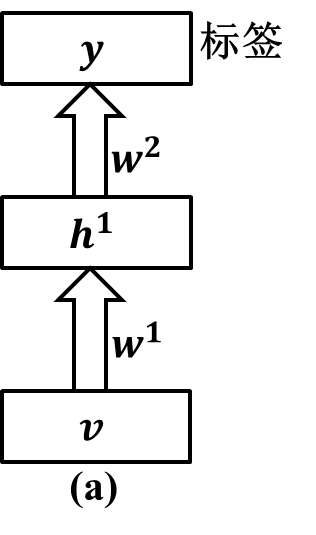
\includegraphics[height=4cm]{images/BP_pretraining1.jpg}
  \end{varwidth}
  \qquad\qquad
  \begin{varwidth}[t]{\textwidth}
    \vspace{0pt}
    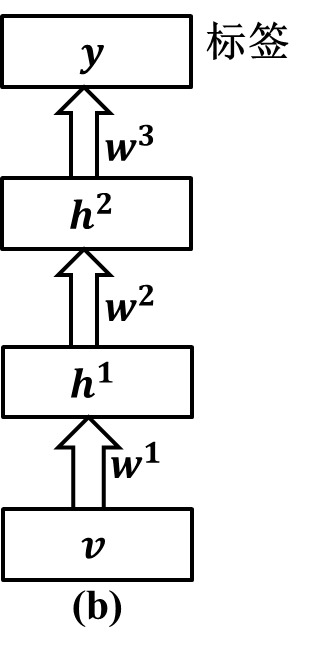
\includegraphics[height=4cm]{images/BP_pretraining2.jpg}
  \end{varwidth}
  \caption{BP预训练示意图}
  \label{fig:BP预训练示意图}
\end{figure}
            % \textcolor[rgb]{1 0 0}{todo:图片:BP预训练示意图}\\
            得到权重$W^{(1)}$;\ding{173}接着在$h^{(1)}$和输出层之间插入一个新的隐含层$h^{(2)}$,再用BP算法训练$v,h^{(1)},h^{(2)},y$,得到$W^{(2)}$;\ding{174}如此下去,知道插入$h^L$个隐含层,收敛后得到$W^{(L)}$。对于采用哪个$W^{(1)}$来进行\ding{173}的训练,我们可以:使用\ding{173}中训练的$W^{(2)}$,在堆积成DBM时不用此$W^{(2)}$;可以都采用\ding{173}中的$W^{(2)}$;可以采用\ding{172}中的$W^{(1)}$,在\ding{173}中不对$W^{(1)}$训练。
            \par
            逐层BP和逐层贪心算法相似,但在BP算法中,每次新的隐含层加入时,所有的层都联合更新,而在逐层贪心算法中,底层权重对上层权重一无所知,因而,大多数情况下,BP算法是较优的。然而,逐层BP有一个缺点:一些隐含层节点可能在训练收敛后处于饱和状态,因此,当新的隐含层加入训练时,很难进行更新。为了解决这个问题,我们可以是用数据的$\frac{1}{L}$来进行训练。
        \subsubsection{混合式预训练}
            \par
            前面提到过生成式预训练和监督式预训练,自然想到将二者合并。已经证明生成式预训练有助于训练深层结构。然而,随着深度的增加,鉴别式预训练同样表现的很好,甚至更好。混合预训练则要优于二者。我们已经注意到,当训练集足够大时,预训练就变得不那么重要了。
        \subsubsection{丢弃式预训练}
            \par
            可以把dropout视为通过随机丢弃神经元来减小DNN容量的方法,也可以把dropout视为一种打包技术,它可以对大量绑定参数的模型做平均,换句话所,与不适用dropout的DNN相比,dropout能够生成更加平滑的目标平面,与一个陡峭的目标平面相比,一个平滑的目标平面有较少的劣性局部最优点,这样,不容易陷入局部极小点。这启发我们可以使用dropout预训练快速找到一个较好的起始点,然后不用dropout来微调DNN。

    \subsection{高斯RBM}
        \par
        前面讨论的BM、RBM、DBN和DBM其输入数据都要求是01二值数据,并且网络中的神经元状态都是01随机变量,即伯努利分布。下面将介绍一些实值RBM,其概率取值不再是01,而是实值。
        \paragraph{高斯-伯努利RBM}在伯努利RBM中,条件概率$p(h|v),p(v|h)$定义为
        \begin{align*}
        & p(h|v) = \sigma (vW +a)\\
        & p(v|h) = \sigma (W^\mathrm{T}h+b)
        \end{align*}
        现在将$v$改为高斯分布,即
        \begin{align*}
        p(v|h) =N(v|Wh,\beta^{-1})
        \end{align*}
        其中:$\beta^{-1}$为协方差矩阵,是一个对角矩阵。注意,这里我们仅将$v$层改为高斯分布,$h$层仍为伯努利分布。对上面的分布取对数,有
        \begin{align*}
        \log N(v|Wh,\beta^{-1}) = -\frac{1}{2} (v-Wh)^\mathrm{T}\beta (v-Wh) + f(\beta)
        \end{align*}
        其中:$f$封装了所有参数,但不包含模型中的随机变量。我们可以忽略$f$,因为它唯一的作用是归一化分布。如果在能量函数中包含$\log N$中涉及到$v$的所有项,并且不添加其它涉及$v$的项,那么,我们的能量函数就能表示想要的条件分布$p(v|h)$。其它条件分布$p(h|v)$比较自由。注意到$\log N$中包含一项
        \begin{align*}
        \frac{1}{2} h^\mathrm{T}W^\mathrm{T}\beta Wh
        \end{align*}
        该项中已经包含$h_i,h_j$项,这一项不能被包含在其中,因为它对应着隐含层单元的边,如果包含这些项,将得到一个线性因子模型,而不是RBM。在RBM中,我们简略的去掉$h_i,h_j$的交叉项,并且忽略这些想不改变条件分布$p(v|h)$。如果我们使用精确地对角矩阵$\beta^{-1}$,会发现对于每个隐含层神经元$h_i$,有
        \begin{align*}
        \frac{1}{2}h_i \sum_j \beta_j W_{ji}^2
        \end{align*}
        \par
        如果在能量函数中包含此项,则当该单元的权重较大且以高进度连接到可见单元时,偏置$h_i$将自动关闭,是否包含该项不影响模型可以表示的分布族,但它会影响模型的学习动态,包含它可以帮助隐含层神经元保持合理激活。因此,在高斯-伯努利RBM中,能量函数定义为
        \begin{align*}
        E(v,h) = \frac{1}{2} v^\mathrm{T}(\beta \odot v) - (v\odot \beta)^\mathrm{T} Wh -a^\mathrm{T} h
        \end{align*}
        并且,我们还可以添加额外项。注意到,上面并没有在可视层$v$中添加偏置。关于如何确定$\beta^{-1}$,可以根据样本数据给出,也可以通过模型估计出。
    \subsubsection{条件协方差无向模型}
        \par
        虽然高斯RBM已经成为实值数据的标准能量模型,但2010.Ranzato认为,高斯RBM不能很好的适应某些类型的实值数据中存在的统计变化,特别是自然图像。图像中的大多数有用的信息在于像素之间的关系,而不是原始像素值。由于高斯RBM反对给定$h$的输入$v$的改建均值建模,所以它不能捕获条件协方差信息。为了解决这一问题,Ranzato提出mean and covariance RBM(mcRBM)、mean product of student-distribution(mPoT)和pike and slab RBM(ssRBM)。
        \paragraph{mcRBM} mcRBM使用隐含层神经元单独的编码所有可视层神经元的条件均值和协方差。具体来所,mvRBM的隐含层分成两组:均值神经元和协方差神经元。对条件均值建模的那组神经元是简单的高斯RBM,另一半是协方差RBM(Ranzato.2010)。对条件协方差的结构进行如下建模:将$h$分为二值均值神经元$h^{(m)}$和二值协方差神经元$h^{(c)}$,mcRBM的能量函数定义为二者的组合
        \begin{align*}
        E_{mc}(x,h^{(m)},h^{(c)}) = E_m(x,h^{(m)}) + E_c(x,h^{(c)})
        \end{align*}
        其中:$E_m$为高斯-伯努利RBM的能量函数
        \begin{align*}
        E_m(x,h^{(m)})  = \frac{1}{2} x^\mathrm{T}x - \sum_j x^\mathrm{T}W_{\cdot j}h_h^{(m)} - \sum_ja_j{(m)}h_j^{(m)}
        \end{align*}
        $E_c$为cRBM的能量函数
        \begin{align*}
        E_c(x,h^{(c)})  = \frac{1}{2} \sum_j h_j^{(c)} \left( x^\mathrm{T}r ^{(j)} \right) ^2 - \sum_ja_j^{(c)} h_j^{(c)}
        \end{align*}
        参数$r^{(j)}$是与$h^{(j)}$关联的协方差权重向量,$a^{(c)}$是一个协方差偏置向量。
        \par
        组合后的能量函数定义的联合分布为
        \begin{align*}
        P_{mc}(x,h^{(m)},h^{(c)}) = \frac{1}{Z}\exp\{-E_{mc}(x,h^{(m)},h^{(c)})\}
        \end{align*}
        给定$h^{(m)}$和$h^{(c)}$后,关于数据的条件分布为(多元高斯分布)
        \begin{align*}
        P_{mc}(x|h^{(m)},h^{(c)})  = N \left( x\ \Big| \ C_{x|h}^{mc} \Big( \sum_jW_{\cdot j}h_j^{(m)} \Big),C_{x|h}^{mc}   \right)
        \end{align*}
        注意,协方差矩阵$C_{x|h}^{mc} = (\sum_j h_j^{(c)}r^{(j)} r^{(j)}{}^\mathrm{T}+I)^{-1}$是非对角矩阵,且$W$是与对条件均值建模的高斯RBM相关联的权重矩阵,对于非对角的条件协方差接哦古,难以通过对比散度(CD)或持续对比散度(PCD)来训练mcRBM。CD和PCD要从$x,h^{(m)},h^{(c)}$的联合分布中采样,这在标准RBM中是通过吉布斯在条件分布上采样实现的,但是在mcRBM中,从$P_{mc}(x|h^{(m)},h^{(c)})$中抽样需要在学习的每个迭代步中计算$(C^{mc})^{-1}$。当样本数据很大时,这是不易的。2010.Ranzato和Hinton通过使用mcRBM自由能上的哈密顿混合蒙特卡罗直接从边缘分布$p(x)$中采样。\\
        注:自由能FreeEnergy(x)定义为
        \begin{align*}
        FreeEnergy(x) = -\log \sum_h e^{-E(x,h)}
        \end{align*}

        \paragraph{学生t分布均值乘积模型}mPoT模型是由2010.Ranzato以类似mcRBM扩展cRBM的方式扩展了PoT模型(2003.Welling)。与mcRBM一样,样本上的PoT条件分布为多元高斯分布,具有非对角的协方差;与mcRBM不同的是,隐含变量的补充条件分布是由条件独立的Gamma分布给出的。mPoT的能量函数为
        \begin{align*}
        &E_{mPoT} \left( x,h^{(m)},h^{(c)} \right) \\
        ={}& E_m \left( x,h^{(m)} \right) + \sum_j \left( h_j^{(c)}\left( 1+\frac{1}{2}\left( r^{(j)}x \right)^2  \right)+ \left( 1-r^{(j)} \right) \log h_j^{(c)}   \right)
        \end{align*}
        其中:$r^{(j)}$是与神经元$h_j^{(c)}$相关联的协方差权重向量。和mcRBM一样,mPoT也无法从非对角高斯条件分布$P_{mPoT}(x|h^{(m)},h^{(c)})$中采样,Ranzato etal(2010)同样采用哈密顿混合蒙特卡洛直接从边际分布$p(x)$中采样。

\section{自动编码器AE}
    \subsection{基础自动编码器AE}
        \par
        我们从主成分分析PCA谈起(不详,可以参考其它的机器学习书籍或者多元统计教材)。设共有$n$个变量和$m$个样本,样本集为$S=\{x^1,x^2,\dots,x^m\}$,$x^k = (x_1^k,x_2^k,\dots,x_n^k)\in R^n$。主成分分析的目标是(仅对无标签数据而言):
        \begin{align*}
        & h_1 = w_{11}x_1 + w_{12}x_ 2+ \dots + w_{1n}x_n = \sum_{i=1}^n w_{1i}x_i\\
        & h_2 = w_{21}x_1 + w_{22}x_ 2+ \dots + w_{2n}x_n = \sum_{i=1}^n w_{2i}x_i\\
        & \qquad \vdots\\
        & h_n = w_{n1}x_1 + w_{n2}x_ 2+ \dots + w_{nn}x_n = \sum_{i=1}^n w_{ni}x_i
        \end{align*}
        换句话说,我们对原本的$n$个变量进行了$n$次(不同的)线性变换,重新得到了$n$个变量(成分)$h_i(i=1,2,\dots,n)$,由于要在$n$个$h_i$中挑去一部分重要的$h_i$,所以叫做主成分。可以对原始变量$x = (x_1,x_2,\dots,x_n)$进行任意的线性变换,显然不能这么做,我们希望$h_i = w_i^\mathrm{T}x$的方差尽可能大,而且各个$h_i$之间相互独立,由于
        \begin{align*}
        Var(h_i) = Var(w_i^\mathrm{T}x) = w_i^\mathrm{T}\Sigma w_i
        \end{align*}
        其中:$\Sigma$为$x$的协方差矩阵。而对于$\forall c$,有
        \begin{align*}
        Var(cw_i^\mathrm{T}x) = cw_i^\mathrm{T}\Sigma w_i c = c^2w_i^\mathrm{T}\Sigma w_i
        \end{align*}
        如果不对$w_i$加以限制,则$Var(h_i)$可以任意增大,问题将变得没有意义。为此,我们要求:\ding{172}
        \begin{align*}
        w_i^\mathrm{T}w_i = 1 \quad i=1,2,\dots,n
        \end{align*}
        即
        \begin{align*}
        w_{i1}^2+w_{i2}^2+\dots+w_{in}^2 = 1 \quad i=1,2,\dots,n
        \end{align*}
        \ding{173}$h_1$是$x_1,\dots,x_n$的线性组合中方差最大的,$h_2$为$x$线性组合的方差第二大,且$h_2$与$h_1$不相关$\dots$,称$h_1,h_2,\dots,h_n$为$x_1,x_2,\dots,x_n$的$n$个主成分。可以将PCA表示成如图(\ref{fig:PCA网络结构示意图})网络结构
            \begin{figure}[H]
            \centering
            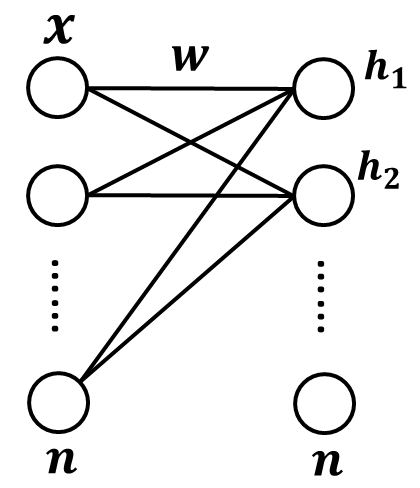
\includegraphics[height=4cm]{images/PCA_net_structure.jpg}
            \caption{PCA网络结构示意图}
            \label{fig:PCA网络结构示意图}
            \end{figure}
        % \textcolor[rgb]{1 0 0}{todo:图片:PCA网络结构示意图}
        \par
        将PCA写成矩阵的形式,有
        \begin{align*}
        h = W^\mathrm{T}x
        \end{align*}
        样本数据$X$是多大,返回的$n$个主成分$h$的数据矩阵$H$就是多大。我们说这些主成分$h_1,h_2,\dots,h_n$中包含了$x$的所有信息,$h_1$是主要成分,$h_2$是第二主要成分。我们自然希望通过$h$来还原$x$,如果考虑所有主成分,则
        \begin{align*}
        x = W^{-1}h
        \end{align*}
        这样就把$x$还原回来了,无损失还原,$x$还是$x$。但是,既然PCA叫做主成分,我们自然希望去掉一些成分,仅保留少量的主成分。这样,还原回来的$x$不再是原本的$x$,但是其主要特征还在。这里,我们打算用$n_k<n$个主成分来还原$x$,还原回来的$x$记为$\hat{x}$,显然$x$和$\hat{x}$不相等。设从$h$到$\hat{x}$的映射为$\hat{x} = g(h)$,画出其网络结构,如图(\ref{fig:PCA网络结构示意图2})
            \begin{figure}[H]
            \centering
            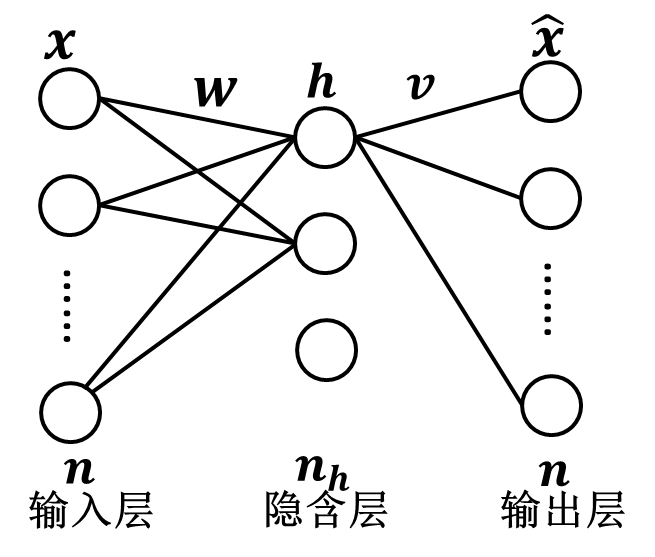
\includegraphics[height=4cm]{images/PCA_net_structure2.jpg}
            \caption{PCA网络结构示意图}
            \label{fig:PCA网络结构示意图2}
            \end{figure}
        % \textcolor[rgb]{1 0 0}{todo:图片:PCA网络结构示意图2}\\
        其中:输入层$x$有$n$个神经元,输出层$\hat{x}$有$n$个神经元,隐含层/主成分层$h$有$n_h<n$个神经元。输入层到隐含层的权重为$W$,隐含层到输出层的权重为$V$,阈值分别为$a,b$。
        \par
        主成分分析是对变量$x$的有损是压缩与还原的过程:$x\xrightarrow{\text{压缩}}h\xrightarrow{\text{还原}}\hat{x}$。或者说PCA是编码和解码过程:将$x$编码到低维空间$h$,在解码到高维空间$\hat{x}$。并且,值得一提的是,如果$x_1,x_2,\dots x_n$之间不相关,只要$n_h<n$,就不能完全还原$x$。现在,将这种思想一般化:编码解码。自动编码器AE即是基于这种思想的神经网络。
        \par
        自动编码器即对自身$x$进行编码解码后还原到$x$。当然,像上面分析的那样,如果对$h$不做任何约束,那么$\hat{x} = g(h) = g(f(x))$是没有任何意义的,因为总会存在映射$f$,将$x$编码解码后还原到$x$。但如果我们对隐含层/特征层$h$加以约束,就会使$h$尽可能保留$x$的特征,以便于还原。使用上面的网络格式
        \begin{align*}
        & h = f(W^\mathrm{T}x+a)\\
        & \hat{x} = g(V^\mathrm{T}h+b)
        \end{align*}
        其中:$f$为编码器,$g$为解码器。进一步,可以写为
        \begin{align*}
        \hat{x} = g(f(x))
        \end{align*}
        由于输入$x$和输出$\hat{x}$的大小相同,我们将AE的网络结构进行折叠,折叠前后的网络结构如图(\ref{fig:AE折叠的网络结构})所示
            \begin{figure}[H]
            \centering
            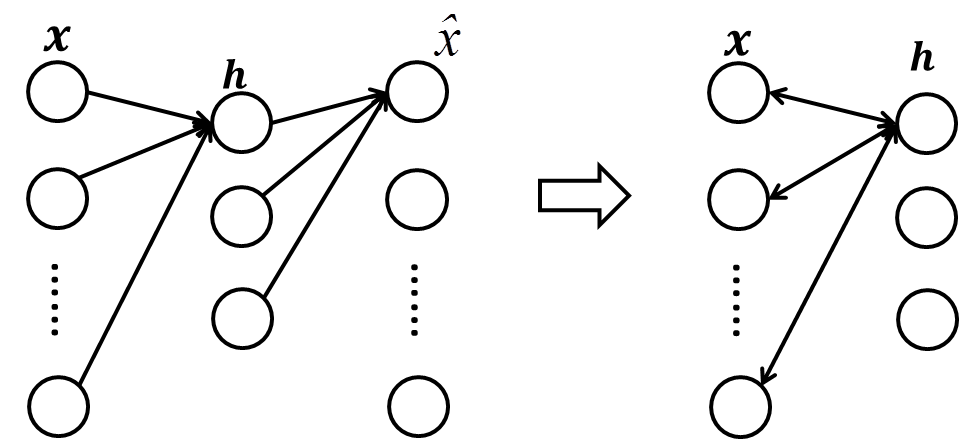
\includegraphics[height=3cm]{images/AE_fold_net_tructure.jpg}
            \caption{AE折叠的网络结构}
            \label{fig:AE折叠的网络结构}
            \end{figure}
        % \textcolor[rgb]{1 0 0}{todo:图片:AE折叠的网络结构}
        \par
        AE的网络结构已经建立起来了,下面的工作就是求解编码器$f$和解码器$g$。这里的函数$f,g$是事先确定的,所以我们的目标是求$W,V,a,b$。我们仍然假设有样本集$S = \{x^{1},x^{2},\dots,x^{m}\}$,$x^{k} = (x_1^k,x_2^k,\dots,x_n^k)\in R^n$。此数据为无标签/无目标的用于无监督的数据。像BP神经网络那样,我们自然想到:求$\theta\triangleq (W,V,a,b)$,来使“离差平方和”尽可能小
        \begin{align*}
        \min_\theta \ J(W,V,a,b) = \sum_{k=1}^m||x^k -\hat{x}^k|| = \sum_{k=1}^m e_k^\mathrm{T}e^k
        \end{align*}
        注意到,这里的离差$e$是一个和$x$同大小的矩阵,$e_k$为$e$的第$k$行,是一个向量。当然,我们可以将目标$J(\theta)$进行正则化,有
        \begin{align*}
        \min_\theta \ J(W,V,a,b) = \sum_{k=1}^m ||x^k - \hat{x}^k|| + \frac{1}{2} ||W||^2 + \frac{1}{2}||V||^2
        \end{align*}
        我们将上述目标一般化,有
        \begin{align*}
        \min_\theta \ J(\theta)= \sum_{k=1}^m \ell(x^k,\hat{x}^k) + \Omega (\theta) = L(x,\hat{x}) + \Omega(\theta)
        \end{align*}
        其中:$\ell$为损失函数,$\Omega(\theta)$为正则项/罚项。\\
        注:1.对$h$的要求:可以令$n_h < n$,也可以要求$h$具有稀疏性;2.此网络深度可以像BP网络那样加深,同样,也可以对其进行堆积。
        \par
        下面来求上述目标$J(\theta)$。从自动编码器的网络结构来看,其网络层数明显可以加深。我们设其层数为$L$,第$l$层的权重为$W^{l},l=1,2,\dots,L$,第$l$层的阈值为$b^{l},l=2,3,\dots,L$。各层神经元数目为$n^{l},l=1,2,\dots,L$,且$n^{1} = n^{L} = n$。优化目标为
        \begin{align*}
        \min_\theta\ J(W,b) = \sum_{k=1}^m ||x^k - \hat{x}^k||^2 + \frac{1}{2}\sum_{l=1}^L||W^l||^2
        \end{align*}
        将$J$关于$\theta$求导,有
        \begin{align*}
        \frac{\partial J}{\partial \theta} = \sum_{k=1}^m\frac{\partial }{\partial \theta}||x^{k} - \hat{x}^k||^2 + \frac{1}{2}\sum_{l=1}^L \frac{\partial }{\partial \theta}||W^l||^2
        \end{align*}
        我们来看
        \begin{align*}
        \frac{\partial }{\partial \theta}||x^{k} - \hat{x}^k||^2  = \frac{\partial }{\partial \theta}\sum_{j=1}^{n}(x_j^k - \hat{x}_j^k)^2
        \end{align*}
        其解法与前面的BP神经网络相似,这里就不再介绍了。
    \subsection{稀疏自动编码器Sparse AE}
        \par
        在前面的AE中,要求$n_h<n$,现在考虑$n_h \geqslant n$。对此,如果不加限制,则编码器不能很好的工作,所以要对$h$加以限制/约束。我们给$h$中神经元加上稀疏约束,具体而言,当神经元的输出接近1的时候,我们认为它被激活,而输出值接近0的时候,它被限制。我们使$h$中的神经元大部分时间都被限制,此即为$h$的稀疏性约束。设$f$为sigmoid(如果是tanh,则当输出为-1时神经元被限制),记稀疏性惩罚为$\Omega(h)$,则目标变为
        \begin{align*}
        J_{sparse}(W,b) = J(W,b) + \Omega (h)
        \end{align*}
        其中:如果仅考虑一个隐含层$h$,则$W = (W^{(1)},W^{(2)})$,$b= (b^{(1)},b^{2})$。
        \par
        用$a_j$表示隐含层神经元$j$得到激活度(输出),但这并未标明是哪一个样本$x^k$带来的激活度(每输入一个样本,都会有一个神经元$j$都会有一个激活度)。所以,我们用$a_j(x^k)$表示样本$x^k$带来的激活度。进一步,用
        \begin{align*}
        \hat{\rho}_j = \frac{1}{m} \sum_{k=1}^m \left( a_j(x^k) \right)
        \end{align*}
        表示$h$的第$j$个神经元的样本平均激活度。我们可以近似的加入一些限制,比如
        \begin{align*}
        \hat{\rho}_j = \rho
        \end{align*}
        其中:$\rho$为稀疏性常数,一般设置为$0.05$。换句话说,我们想让$j$的平均激活度为0.05。为了满足这一要求,隐含层$j$的激活度庇护接近于0。现在,我们写出稀疏性罚因子$\Omega(h)$的具体形式
        \begin{align*}
        \sum_{j=1}^{n_h} \left[ \rho\log\frac{\rho}{\hat{\rho}_j}+ (1-\rho)\log\frac{1-\rho}{1-\hat{\rho}_j}  \right]
        \end{align*}
        注意,我们仅考虑一个隐含层的AE,$n_h$为隐含层神经元个数。其实,上式是一个以$\rho$为均值和一个以$\hat{\rho}_j$为均值的2个伯努利随机变量之间的相对熵
        \begin{align*}
        KL(\rho||\hat{\rho}_j) = \left[ \rho\log\frac{\rho}{\hat{\rho}_j}+ (1-\rho)\log\frac{1-\rho}{1-\hat{\rho}_j}  \right]
        \end{align*}
        在KL中,当$\hat{\rho}_j = \rho$时,它达到最小值0,而当$\hat{\rho}_j$靠近0或者1时,相对熵KL会变的非常大。所以这个$\Omega(h)$是有效的,于是目标写为
        \begin{align*}
        J_{sparse}(W,b) &= J(W,b) + \Omega (h)\\
        &= \sum_{k=1}^m ||x^k-\hat{x}^k||^2 + \frac{\beta}{2}\sum_{j=1}^{n_h}KL(\rho||\hat{\rho}_j)
        \end{align*}
        注意;上面的目标中不包含正则项,或者说$KL$就是正则项。现在求$J_{sparse}$的导数,$J_{sparse}$求导由两部分组成:一个是$J(W,b)$求导,一个是$KL$求导。$J(W,b)$的求导和BP相似,所以下面主要介绍$KL$的求导。
        \par
        记$S(W,b) = \sum_{j=1}^{n_h}KL(\rho||\hat{\rho}_j)$,我们要求导
        \begin{align*}
        & \frac{\partial S(W,b)}{\partial W_{ij}^{(l)}}\\
        & \frac{\partial S(W,b)}{\partial b_i^{(l)}}
        \end{align*}
        \par
        首先,我们将$S(W,b)$展开,有
        \begin{align*}
        S(W,b) = \sum_{j=1}^{n_h}KL(\rho||\hat{\rho}_j) =\sum_{j=1}^{n_h} \left[ \rho\log\frac{\rho}{\hat{\rho}_j}+ (1-\rho)\log\frac{1-\rho}{1-\hat{\rho}_j}  \right]
        \end{align*}
        其中:
        \begin{align*}
        \hat{\rho}_j = \frac{1}{m} \sum_{k=1}^m a_j(x^k) = \frac{1}{m}\sum_{k=1}^m f \left( \sum_{i=1}^{n^1}x^k_i W_{ij}^{(1)}  + b_j^{(1)}\right)
        \end{align*}
        由上式可知:
        \begin{enumerate}
        \item 当$l \neq 1$时,$\frac{\partial S(W,b)}{\partial W_{ij}^{(l)}} = 0
        ,\frac{\partial S(W,b)}{\partial b_j^{(l)}}=0$;
        \item
        \begin{align*}
        & \frac{\partial S(W,b)}{\partial W_{ij}^{(l)}} = \frac{\partial }{\partial W_{ij}^{(l)}}\sum\limits_{j=1}^{n_h} KL(\rho||\hat{\rho}_j) = \frac{\partial KL(\rho||\hat{\rho}_j)}{\partial W_{ij}^{(l)}}\\
        & \frac{\partial S(W,b)}{\partial b_j^{(l)}} = \frac{\partial }{\partial b_j^{(l)}}\sum\limits_{j=1}^{n_h} KL(\rho||\hat{\rho}_j) = \frac{\partial KL(\rho||\hat{\rho}_j)}{\partial b_j^{(l)}}
        \end{align*}
        \end{enumerate}
        由上述两条,我们有
        \begin{align*}
        \frac{\partial S(W,b)}{\partial W_{ij}^{(1)}} & = \frac{\partial KL(\rho||\hat{\rho}_j)}{\partial W_{ij}^{(1)}}\\
        & = \frac{\partial }{\partial W_{ij}^{(1)}} \left[ \rho\log\frac{\rho}{\hat{\rho}_j}+ (1-\rho)\log\frac{1-\rho}{1-\hat{\rho}_j}  \right]\\
        &= \frac{\partial }{\partial W_{ij}^{(1)}} \Big\{ \rho(\log\rho - \log \hat{\rho}_j) + (1-\rho)[\log(1-\rho) -\log(1-\hat{\rho}_j)  ]  \Big\}\\
        &= \rho \left( 0- \frac{1}{\hat{\rho}_j} \frac{\partial \hat{\rho}_j}{\partial W_{ij}^{(1)}} \right) (1-\rho) \left( 0+\frac{1}{1-\hat{\rho}_j}\frac{\partial \hat{\rho}_j}{\partial W_{ij}^{(1)}} \right) \\
        &= \left( -\frac{\rho}{\hat{\rho}_j }+ \frac{1-\rho}{1-\hat{\rho}_j} \right) \frac{\partial \hat{\rho}_j}{\partial W_{ij}^{(1)}}
        \end{align*}
        类似的,有
        \begin{align*}
        \frac{\partial S(W,b)}{\partial b_j^{(1)}} =  \left( -\frac{\rho}{\hat{\rho}_j }+ \frac{1-\rho}{1-\hat{\rho}_j} \right) \frac{\partial \hat{\rho}_j}{\partial b_j^{(1)}}
        \end{align*}
        \par
        接下来,只需要求出$\hat\rho_j$的导数即可。由$\hat\rho_j$的计算公式,我们有
        \begin{align*}
        \hat{\rho}_j = \frac{1}{m} \sum_{k=1}^m a_j(x^k) = \frac{1}{m}\sum_{k=1}^m f \left( \sum_{i=1}^{n^1}x^k_i W_{ij}^{(1)}  + b_j^{(1)}\right)
        \end{align*}
        为书写方便,令
        \begin{align*}
        & z_j^{(2)} =z_j^{(2)}(x^k)= \sum_{i=1}^{n^1}x^k_i W_{ij}^{(1)}  + b_j^{(1)}\\
        & a_j(x^k)= f \left( z_j^{(2)} \right)
        \end{align*}
        于是有
        \begin{align*}
        \frac{\partial \hat{\rho}_j}{\partial W_{ij}^{(1)}} & = \frac{1}{m} \sum_{k=1}^m f'\left( z_j^{(2)} \right) \frac{\partial z_i^{(2)}}{\partial W_{ij}^{(1)}}\\
        & = \frac{1}{m} \sum_{k=1}^m f'\left( z_j^{(2)} \right) x_i^k
        \end{align*}
        类似的,有
        \begin{align*}
        \frac{\partial \hat{\rho}_j}{\partial b_j^{(1)}} & = \frac{1}{m} \sum_{k=1}^m f'\left( z_j^{(2)} \right) \frac{\partial z_i^{(2)}}{\partial b_j^{(1)}}\\
        & = \frac{1}{m} \sum_{k=1}^m f'\left( z_j^{(2)} \right)
        \end{align*}
        至此,求导工作结束。作为练习,可以将上述内容写为矩阵形式。
    \subsection{降噪自动编码器Denoising AE}
        \par
        Denoise AE由Vincent\cite{2008.Vincent}于2008年提出。其主要思想是:首先,对样本数据$S= \{x^k\}_{k=1}^m$加入噪声。然后,基于有噪声的输入向量(样本)做编码解码。要求解码后的向量尽可能保持在原输入向量周围。如果AE对干扰后的数据都能很好的还原,则此网络具有很好的鲁棒性。
        \par
        设原始数据为$x$,加入噪声后的输入为$\tilde{x}=x+noise$,然后将$\tilde{x}$通过编码函数$f$映射到$h$,在解码$h$到$\hat{x} = g(h)$,表达式写为
        \begin{align*}
        & h = f(\tilde{x}) = \sigma (W\tilde{x}+a)\\
        & \hat{x} = g(h) = \sigma (Vh+b)
        \end{align*}
        \par
        损失函数用$\hat{x}$与$x$来定义,而非$\hat{x}$与$\tilde{x}$,有
        \begin{align*}
        J_{DAE}(W,b) = \sum_{k=1}^m \ell(x^k,\hat{x}^k)
        \end{align*}
        其中:$W=(W^{(1)}, W^{(2)}) = (W,V) $。Denoise AE的关键是对输入$x$加干扰,目前常用的干扰有2种:\ding{172}
        \begin{align*}
        & \tilde{x} = x+\varepsilon\\
        & \varepsilon \sim N(0,\sigma^2I)
        \end{align*}
        \ding{173}就单一样本而言,以概率$p$将输入向量$x^k$的部分量设置为0,其余不变。\\
        注:前面的AE我们都是采用离差平方和最小,还可以考虑极大似然方法,这一点很重要!
    \subsection{边缘降噪自动编码器mDAE}
        \par
        Chen.M于2014年开发了边缘降噪自动编码器(Marginalized Denoising AE,mDAE)\cite{2014.Chen}。在Denoise AE中,目标函数定义为
        \begin{align*}
        J_{DAE}(\theta) = \sum_{k=1}^m \ell \left( x^k,g(f(\tilde{x})) \right)
        \end{align*}
        令上式中的$g(f(\tilde{x})) = f_\theta(\tilde{x})$(这里的$f_\theta$不是$f$),$\mu_x = \mathbb{E}_{p(x|\tilde{x})}[\tilde{x}]$,其中:$\tilde{x}$为$x$的干扰项,$\mu_x$是$\tilde{x}$的期望值。我们的目标是
        \begin{align*}
        \frac{1}{m} \sum_{k=1}^m \frac{1}{n} \sum_{j=1}^n \ell \left( x_j^k,f_\theta \left( \tilde{x}_j^k \right)  \right)
        \end{align*}
        当隐含层$h$的神经元个数很多时,会使得学习速度变得很慢。上面的目标本质是
        \begin{align*}
        \frac{1}{m} \sum_{k=1}^k \mathbb{E}_{p(\tilde{x}^k|x^k)}[\ell (x^k,f_\theta(\tilde{x}^k))  ]
        \end{align*}
        将损失函数$\ell$在$\tilde{x}$处二阶泰勒展开,有
        \begin{align*}
        \ell \left( x^k,f_\theta(\tilde{x}^k) \right) \approx \ell (x,f_\theta(\mu_x))+(\tilde{x} - \mu_x)^\mathrm{T}\nabla_{\tilde{x}} \ell+ \frac{1}{2}(\tilde{x} - \mu_x)^\mathrm{T}\nabla_{\tilde{x}}^2 \ell \cdot (\tilde{x} - \mu_x)
        \end{align*}
        其中:$\nabla_{\tilde{x}}\ell,\nabla_{\tilde{x}}^2\ell$是$\ell$在$\tilde{x}$处的一阶导数和二阶导数。
        \par
        对$\tilde{x}$取期望
        \begin{align*}
        \mathbb{E} [\ell(x,f_\theta(\tilde{x}))] \approx \ell (x,f_\theta(\mu_x)) + \frac{1}{2} \mathrm{tr} \left( \mathbb{E}[(\tilde{x} - \mu_x)(\tilde{x} - \mu_x)^\mathrm{T} ]\nabla_{\tilde{x}}^2 \ell\right)
        \end{align*}
        其中:$\mathbb{E}[\tilde{x}] = \mu_x$。令$\Sigma_x = \mathbb{E}[(\tilde{x} - \mu_x)(\tilde{x} - \mu_x)^\mathrm{T} ]$,则上式写为
        \begin{align*}
        \mathbb{E} [\ell(x,f_\theta(\tilde{x}))] \approx \ell (x,f_\theta(\mu_x)) + \frac{1}{2} \mathrm{tr} \left(\Sigma_x \nabla_{\tilde{x}}^2 \ell \right)
        \end{align*}
        上式即为损失函数。它只需要基于干扰项$\tilde{x}$的一阶泰勒展开和二阶泰勒展开即可。并且,在$x$中添加噪声时,由于每一个样本是单独加入噪声的,所以$\Sigma_x$可简化为对角矩阵。因此,只需要计算Hesse矩阵$\nabla_{\tilde{x}}^2 \ell$的对角项即可。
        \par
        Hesse矩阵的缩放依赖于数据的维度,但是对角矩阵的缩放是线性的,这种简化可以节省计算量,特别是对于高维数据而言。我们设第$k$个Hessi矩阵的对角为
        \begin{align*}
        \frac{\partial ^2\ell}{\partial \tilde{x}^k{}^2} = \left( \frac{\partial z}{\partial \tilde{x}^k} \right) ^2 \frac{\partial ^2\ell}{\partial z^2} \frac{\partial z}{\partial \tilde{x}^k} +  \left( \frac{\partial \ell}{\partial z} \right) ^\mathrm{T}\frac{\partial ^2z}{\partial \tilde{x}^k{}^2}
        \end{align*}
        其中:$z$为隐含层的输出。按LeCun(1998)提出的方法,将上式的最后一项省略,前一项是一个二次项,矩阵$\nabla_z^2\ell = \frac{\partial ^2\ell}{\partial z^2}$表示$\ell$关于$z$的Hesse矩阵,并且这个矩阵是正定的,所以可以利用正定性进一步简化矩阵的非负对角项。简化之后,该Hessi矩阵的对角项计算公式为
        \begin{align*}
        \frac{\partial ^2\ell}{\partial \tilde{x}^k{}^2} \approx \sum_{j=1}^{n_h}\frac{\partial ^2 \ell}{\partial z_j^2} \left( \frac{\partial z_j}{\partial \tilde{x}^k} \right) ^2
        \end{align*}
        其中:$n_h$为隐含层神经元个数;$z_j$为$h$中第$j$个神经元的输出。经过上面的简化计算之后,mDAE的最终目标函数为
        \begin{align*}
        J_{mDAE}(\theta) = L(x,f_\theta(\mu_x)) + \frac{1}{2}\sum_{k=1}^m \sigma_{x^k}^2 \sum_{j=1}^{n_h}\frac{\partial ^2 \ell}{\partial z_j^2} \left( \frac{\partial z_j}{\partial \tilde{x}^k} \right) ^2
        \end{align*}
        其中:$\sigma_{x^k}^2$是第$k$个样本$x^k$干扰的方差,也即$\Sigma_x$对角矩阵的第$k$个元素。
    \subsection{收缩自动编码器Contractive AE}
        \par
        CAE\cite{2011.Salah}由Salah Rifai等于2011年提出。对于一般的AE,在目标/损失函数后加正则项,其目标函数变为
        \begin{align*}
        J_\Omega(\theta) = L(x,\hat{x})+\Omega(\theta)  = \sum_{k=1}^m\ell(x^k,\hat{x}^k)+\Omega(\theta)
        \end{align*}
        其中:$\Omega(\theta)$为参数$\theta$的正则项,网络的编码解码过程为
        \begin{align*}
        & h=f(Wx^k+a)\\
        & \hat{x^k} = g(Vh+b) = g(Vf(Wx^k+a)+b) = g(f(x^k))
        \end{align*}
        我们这里直接对$\theta$进行惩罚,一般而言,$\Omega(\theta) = \sum_{ij}W_{ij}^2$。
        \par
        现在,仍然对$h$隐含层进行处理,令
        \begin{align*}
        \Omega(h) & = ||J_f(x)||_{\mathcal{F}}^2 =\sum_{ij} \left( \frac{\partial h_j(x)}{x_i} \right)
        \end{align*}
        其中:$J_f(x)$是隐含层输出值关于权重$W$的Jacobi矩阵,$||J_f(x)||_{\mathcal{F}}^2$表示该Jacobi矩阵的$\mathcal{F}$范数的平方,即矩阵中的每个元素求平方再求和,具体写为
        \begin{align*}
        ||J_f(x)||_{\mathcal{F}}^2 = \sum_{i=1}^{n_h} (h_i(1-h_i))^2 \sum_{j=1}^nW_{ij}^2
        \end{align*}
        其计算复杂度为$O(n\times n_h)$。此时的目标函数变为
        \begin{align*}
        J_{CAE}(\theta) = \sum_{k=1}^m \left[ \ell \left( x^k,g(f(x^k)) \right)  + \lambda ||J_f(x^k)||_{\mathcal{F}}^2 \right]
        \end{align*}
        \par
        解释:去噪自动编码器DAE和CAE之间存在一定的联系,Alian和Bengio(2013)指出:在引入小的高斯噪声时,DAE的重构误差与CAE的收缩惩罚因子$\Omega (h)$是等价的,也就是说,CAE具有抵抗微小干扰的能力。CAE只是局部收缩,对样本$x$的所有扰动都映射到$f(x)$的附近。从全局来看,2个不同点$x,x'$,会分别被映射到远离原点的两个点$f(x),f(x')$。CAE对数据中的小扰动敏感性较小,且重构特征不受惩罚因子的影响。但是CAE只对数据中极小扰动有鲁棒性。为此,我们可以进一步惩罚不同阶的偏差,将其目标函数改为
        \begin{align*}
        J_{CAE+h} = \sum_{k=1}^m \ell \left( x^k,g(f(x^k)) \right) + \lambda ||J_f(x)||_{\mathcal{F}}^2+ \gamma \mathbb{E}_\varepsilon [ ||J(x) - J_f(x+\varepsilon)||_{\mathcal{F}}^2  ]
        \end{align*}
        其中:$\varepsilon \sim N(0,\sigma^2 I)$,$\gamma,\lambda$为权重参数,$x+\varepsilon = \tilde{x}$。
        \par
        经过上面的改进,CAE-h的鲁棒性进一步提高。但由于基于鲁棒理论的CAE较为复杂,构建训练的难度较大,因而针对CAE的引用较少。
    \subsection{堆积自动编码器 Stacked AE}
        \par
        1986.Rumelhart提出自动编码器AE;2006.Hinton提出深度置信网络DBN;2007.Bengio提出稀疏自动编码器;2008.Vincont提出去噪自动编码器;2010.Salah提出收缩自动编码器;2011.Jonathan提出卷积自动编码器;2013.Telmo研究了不同代价函数训练得到的深度堆积自动编码器的性能。
        \par
        回忆一下我们是怎样搭建前2个深度网络DBN和DBM的?DBM是一个个小的RBM模型堆积而成,对样本进行学习时,先训练每个小的RBM,然后把它们组合在一起进行微调。即Henton提出的贪心逐层训练算法。其实,AE和RBM存在很多相似的地方:它们都可以用来生成数据(对样本分布进行估计),并且AE也可以表示成RBM的网络形式,如图(\ref{fig:AE折叠成RBM的网络形式})
            \begin{figure}[H]
            \centering
            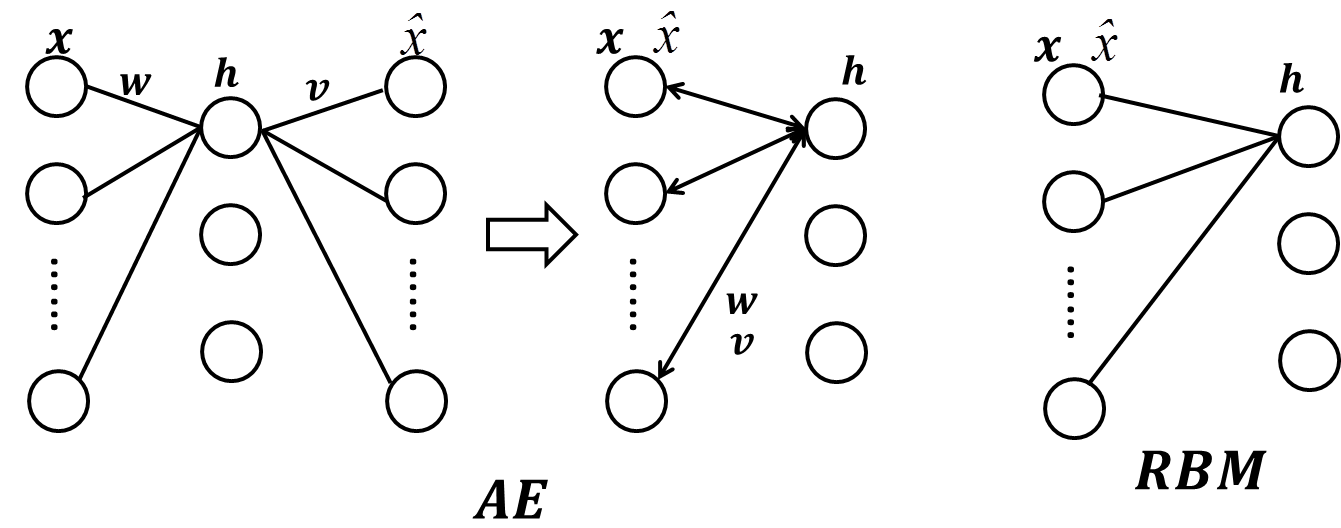
\includegraphics[height=3cm]{images/AE_fold_into_RMB_net.jpg}
            \caption{AE折叠成RBM的网络形式}
            \label{fig:AE折叠成RBM的网络形式}
            \end{figure}
        % \textcolor[rgb]{1 0 0}{todo:图片:AE折叠成RBM的网络形式}\\
        那么自然想:能否将AE堆积形成深度网络?可以的,把AE堆积而成的深度网络称为Deep AE或者stacked AE(注意:这里的AE可以是AE的衍生模型,如CAE和后面介绍的VAE)。
        \par
        DBM是在RBM的隐含层$h$后再添加网络层,那么,AE应该在$h$层/特征层还是在$\hat{x}$层后再加网络层呢?即下一个AE的输入是上一个AE的$h$层还是$\hat{x}$层?在回答这个问题之前,我们来记一下AE
        \begin{align*}
        & h = f(Wx+a)\\
        & \hat{x} = g(Vh+b)
        \end{align*}
        一般情况下,$\hat{x}$不是$x$的精确重构,它只是在满足一定分布的条件概率$p(x|\hat{x})$下,最大程度的接近$x$。因此,AE的目标不仅可以是离差平方和,还可以用极大似然估计,特别是在去噪自动编码器中,$\hat{x}$是有明显(条件)分布的。并且
        \begin{align*}
        \ell (x,\hat{x}) \propto -\log (x|\hat{x})
        \end{align*}
        \par
        如果$x\in R^n$,则$x|\hat{x} \sim N(\hat{x},\sigma^2I)$,这时可以采用离差平方和作为目标$||x-\hat{x}||^2$;如果$x\in \{0,1\}^n$,则$x|\hat{x}\sim B(\hat{x})$,这时就不能用$||x-\hat{x}||$作为目标,就要使用交叉熵等(这个在logistics回归中有介绍)
        \begin{align*}
        \ell (x,\hat{x}) = -\sum_j \left[ x_j\log \hat{x}_j + (1-x_j)\log (1-\hat{x}_j)  \right] = H(B(x)||B(\hat{x}))
        \end{align*}
        \par
        现在考虑我们的问题:下一个AE的输入是上一个AE的$h$层还是$\hat{x}$层?(1)如果是将隐含层$h$作为下一层的输入,那么,预训练(无监督)逐层训练应该为:将第一个AE训练好后,有$W^{(1)},V^{(1)},a^{(1)},b^{(1)}$;然后,将样本再次输入到第一个AE中,每个样本$x^k$都会有一个$h^k,\hat{x}^k$,我们把$h = \{h^k\}_{k=1}^m$作为输入,输入到第二个AE中进行训练,训练后有$W^{(2)},V^{(2)},a^{(2)},b^{(2)}$;然后将$h$在此输入,如此下去,直到最后一层。这样,就完成了stacked AE的预训练,也就得到了深层网络的初始权重和阈值。如果要进行分类任务,可以在预训练之后,运用BP等算法对网络参数进行微调(联合训练)。如图(\ref{fig:SAE的训练过程图})所示
            \begin{figure}[H]
            \centering
            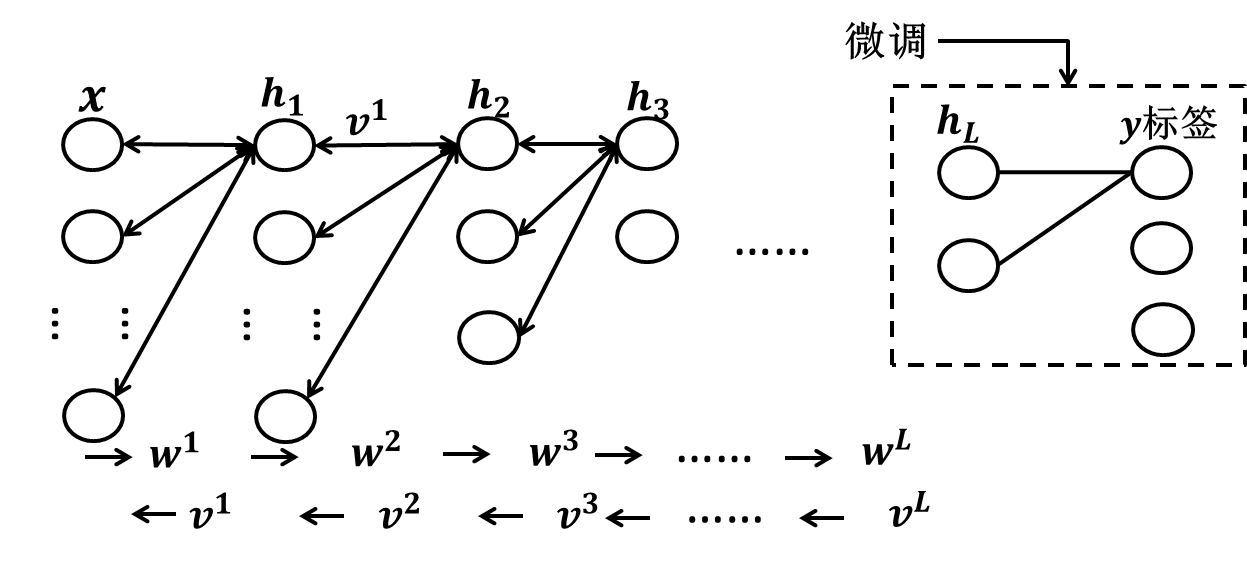
\includegraphics[height=3cm]{images/SAE_training_process.jpg}
            \caption{SAE的训练过程图}
            \label{fig:SAE的训练过程图}
            \end{figure}
        % \textcolor[rgb]{ 1 0 0}{todo:图片:SAE的训练过程图}\\
        注:如果设置$V^\mathrm{T} = W$,那么网络的训练会变得简单易行。(2)如果是将输出层$\hat{x}$作为下一个AE的输入,则其深层网络如图(\ref{fig:AE第二种堆积网络})所示
            \begin{figure}[H]
            \centering
            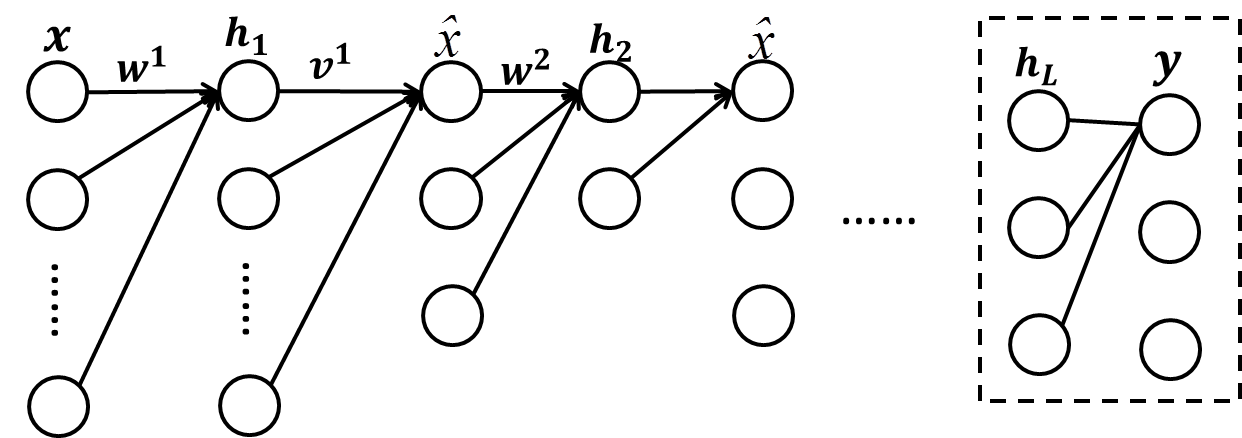
\includegraphics[height=3cm]{images/the_second_accumulation_net_of_AE.jpg}
            \caption{AE第二种堆积网络}
            \label{fig:AE第二种堆积网络}
            \end{figure}
        % \textcolor[rgb]{1 0 0}{todo:图片:AE第二种堆积网络}\\
        其训练过程和(1)的情况是相似的。
    \subsection{变分自动编码器 VAE}
        \par
        记样本数据为$D=\{x^1,x^2,\dots,x^m\}$,$D$是域$S\in R^n$中的采样\footnote{我们可以在实值$R^n$上讨论$x$,也可以在$\{0,1\}^n$上进行讨论。},$x^k = (x_1^k,x_2^k,\dots,x_n^k)\in R^n$称为样本点。并且,我们假设是$n$随机变量$x = (x_1,x_2,\dots,x_n)$,所以$S$上应该有这$n$个随机变量的分布函数$p(x)$。
        \par
        假设AE的隐含层$z\overset{\Delta}{=}h$有$n_h$个神经元,神经元之间可以互相连接,也可以不连接(独立)。记全体隐含层神经元为$z = (z_1,z_2,\dots,z_{n_h})$。假设AE网络的参数$\theta$已经给出,我们可以说:给定$x$后就有了$z$,或者给定$z$之后就有了$x$,因为二者之间是一个编码$f$和解码$g$的过程
        \begin{align*}
        & z = f(x;\theta')\\
        & \hat{x} = g(z;\theta'')
        \end{align*}
        令$\theta \overset{\Delta}{=}(\theta',\theta'')\overset{\Delta}{=}(W,V,a,b)$。值得一提的是,我们可以将$f,g$扩展为任意函数形式,比如MLP, CNN等网络形式。也可以将$z$设置为任意结构,$z$中的神经元之间可以连接、不连接以及部分连接,这样AE模型的范围就变得大了许多。
        \par
        AE网络中的参数$\theta$是待求的,关于$\theta$的求解,大致可分为3个方向:\ding{172}基于参数估计得极大似然估计ML;\ding{173}基于贝叶斯方法的最大后验估计MAP;\ding{174}离差平方最小的最小二乘OLS。三者的共同之处是,它们都是一个优化问题。前面我们讨论了\ding{174}离差平方和方法,下面先来看极大似然估计。
        \par
        在假设样本独立同分布情况下,如果已经知道了单一样本$x^k$的分布 $p_\theta(x^k)\overset{\Delta}{=}p(x^k|\theta) $,可以直接写出极大似然的目标
        \begin{align*}
        \max_\theta\ J(\theta) = \log P(x|\theta) = \log \prod_{k=1}^mp(x^k;\theta) = \sum_{k} \log p(x^k;\theta)
        \end{align*}
        如果样本的分布$p(x^k;\theta)$形式已知,直接求导即可。但是现在的问题是:$p(x;\theta)$不易求解,但是存在一个潜随机变量$z$,$p(x,z;\theta)$是可求的(就像在RBM中遇到的那样)。
        \par
        抛弃我们的模型,如果已知$p(x,z)$,如何求$p(x)$?从联合分布$p(x,z)$中采样$\{x^k,z^k\}$,然后求和/积即可。回到我们的模型中,发现只有部分样本$\{x^k\}$,称$\{x^k,z^k\}_{k=1}^m$为整体样本,$\{x^k\}_{k=1}^m$为部分样本。关于潜变量$z$的取值,仅来源于后验概率分布$p(z|x;\theta)$(即我们建立的模型)。我们记$x$的概率分布为$p(x;\theta)$,$z$的概率分布为$q(z;\theta)$,联合概率分布为$p(x,z;\theta)$,条件分布为$p(x|z;\theta)$和$p(z|x;\theta)$。
        \par
        既然$p(x;\theta)$不易找到,考虑将其用联合分布表示
        \begin{align*}
        p(x;\theta) = \int_zp(x,z;\theta)\mathrm{d}z
        \end{align*}
        于是,单一样本的$x \overset{\Delta}{=}x^k$最大似然目标为
        \begin{align*}
        J(\theta) = \log p(x;\theta) = \int_zp(x,z;\theta)\mathrm{d}z
        \end{align*}
        由条件概率关系
        \begin{align*}
        p(x,z) = p(x)p(z|x) = q(z)p(x|z)
        \end{align*}
        并且我们求$p(x)$,可以得到
        \begin{align*}
        J(\theta) &= \log \int_z p(x,z;\theta)\mathrm{d}z\\
        &=\log \int_z q(z)p(x|z)\mathrm{d}z
        \end{align*}
        注意:上面的概率分布函数都忽略了参数$\theta$。本应写为$p(x;\theta),q(z;\theta)$,并且,如果在贝叶斯框架,则写为$p(x|\theta),q(z|\theta)$。上式的难点在于$q(z)$和$p(x|z)$。下面介绍EM算法和变分估计,并用这两种方法求解上述问题。
        \subsubsection{EM算法}
            \par
            EM算法是Dempster等于1997年提出的,用于求解含有潜变量$z \overset{\Delta}{=}h$的参数极大似然估计或最大后验概率估计。我们假设在$t$次迭代后,参数值为$\theta^t$,现在,我们要求$\theta^{t+1}$。我们自然希望新的参数$\theta$能使目标$J(\theta)$增加,即$J(\theta)>J(\theta^t)$。为此,我们考虑二者的差
            \begin{align}
            \label{极大目标迭代差量}
            J(\theta) - J(\theta^t) = \log \int_z q(z)p(x|z)\mathrm{d}z - \log p(x;\theta^t)
            \end{align}
            \begin{lemma}[Jensen不等式]
            设$\varphi$为凸函数,则
            \begin{align*}
            \varphi(\mathbb{E}(x)) \leqslant \mathbb{E}(\varphi(x)) \Leftrightarrow\varphi \left( \sum_{i=1}^ng(x_i) \lambda_i\right) \leqslant \sum_{i=1}^n\varphi(g(x_i))\lambda_i
            \end{align*}
            其中:$x = (x_1,x_2,\dots,x_n)$,$\sum_i\lambda_i = 1$,$\lambda_i \geqslant 0$。
            \end{lemma}
            注:Jensen不等式给出了积分的凸函数值和凸函数的积分值之间的关系。其实,在SVM部分有简单的介绍过Jensen不等式。
            \par
            将Jensen不等式应用到(\ref{极大目标迭代差量})中,有
            \begin{align*}
            J(\theta) - J(\theta^t) &= \log \int_z q(z)p(x|z)\mathrm{d}z - \log p(x;\theta^t)\\
            &=\log \int_zp(z|x;\theta^t) \frac{p(x|z)q(z)}{p(z|x;\theta^t)}\mathrm{d}t - \log p(x;\theta^t)\\
            & \geqslant \int_zp(z|x;\theta^t) \log\frac{p(x|z;\theta) q(z;\theta)}{p(z|x;\theta^t)}\mathrm{d}t - \log p(x;\theta^t)\\
            &=\int_zp(z|x;\theta^t) \log\frac{p(x|z;\theta) q(z;\theta)}{p(z|x;\theta^t)p(x;\theta^t)}\mathrm{d}t
            \end{align*}
            于是有
            \begin{align*}
            J(\theta) \geqslant J(\theta^t) + \int_zp(z|x;\theta^t) \log\frac{p(x|z;\theta) q(z;\theta)}{p(z|x;\theta^t)p(x;\theta^t)}\mathrm{d}t
            \end{align*}
            令
            \begin{align*}
            B(\theta,\theta^t) = J(\theta^t) + \int_zp(z|x;\theta^t) \log\frac{p(x|z;\theta) q(z;\theta)}{p(z|x;\theta^t)p(x;\theta^t)}\mathrm{d}t
            \end{align*}
            则$B(\theta,\theta^t)$是目标$J(\theta)$的下界,且由$B(\theta^t,\theta^t) = J(\theta^t)$可知,对于任意的$\theta$,如果$\theta$使$B(\theta ,\theta^t)>B(\theta^t,\theta^t)$,则$J(\theta)>J(\theta^t)$。为了使$J(\theta)$尽可能增大,选择$\theta^{t+1}$是$B(\theta,\theta^t)$最大。
            \begin{align*}
            \theta^{t+1} & = \arg \max_\theta B(\theta,\theta^t)\\
            & = \arg \max_\theta J(\theta^t) + \int_zp(z|x;\theta^t) \log\frac{p(x|z;\theta) q(z;\theta)}{p(z|x;\theta^t)p(x;\theta^t)}\mathrm{d}t\\
            & = \arg \max_\theta \int_z p(z|x;\theta^t) \log p(x|z;\theta)q(z;\theta)\mathrm{d}t\\
            & \overset{\Delta}{= } \int_z p(z|x;\theta^t)\log p(x,z;\theta)\mathrm{d}z
            \end{align*}
            令
            \begin{align*}
            Q(\theta,\theta^t) & = \int_z p(z|x;\theta^t)\log p(x,z;\theta)\mathrm{d}z\\
            & \overset{\Delta}{=} \sum_z p(z|x;\theta^t)\log p(x,z;\theta)
            \end{align*}
            $Q$是完整数据$(x,z)$的对数似然函数$\log p(x,z;\theta)$的期望。可以给出如下的EM算法:\\
            \textbf{Step1}.初始化。$D = \{x^k\}_{k=1}^m$。初始网络AE,初始参数$\theta^0$,联合分布函数$p(x,z;\theta)$,迭代次数$t:=0$,$t_{max}$,容许误差$\varepsilon_1,\varepsilon_2$。\\
            \textbf{Step2}.对第$t$次迭代,已经有了$\theta^t$,现在来求$\theta^{t+1}$。
            \begin{enumerate}
            \item E步:计算概率$p(z|x;\theta^t)$;
            \item M步:计算
            \begin{align*}
            & Q(\theta,\theta^t)= \int_z p(z|x;\theta^t)\log p(x,z;\theta)\mathrm{d}z\\
            & \theta^{t+1} = \arg\max_\theta Q(\theta,\theta^t)
            \end{align*}
            \end{enumerate}
            \textbf{Step3}.终止条件。如果$||\theta^{t+1} - \theta^t||<\varepsilon_1$或者$||Q^{t+1} - Q^t||<\varepsilon_2$则终止;否则,则置$t:=t+1$,返回Step2.
            \par
            现在的问题是,如何求解$p(z|x;\theta^t)$、$p(x,z;\theta)$以及$\int_z p\log p\mathrm{d}z$?假设前面已经直达了$p(x,z;\theta)$和$p(z|x;\theta^t)$,现在的关键是如何求积分。我们用数值积分公式计算$Q(\theta,\theta^t)$中的积分,有
            \begin{align*}
            Q(\theta,\theta^t) \approx \frac{1}{N} \sum_{i=1}^N\log p(x,z^i;\theta)
            \end{align*}
            其中:$N$为$z^i$的样本数。这里涉及到按照某分布$p(z|x)$对$z$进行采样$\{z^i\}_{i=1}^N$,我们可以采用MCMC等采样方法。
            \paragraph{MCMC采样}
            MCMC适用于处理给定分布$p(z|x;\theta^t)$,从中采样$z$的问题。由于马尔科夫链能收敛到平稳分布,如果我们能够着一个转移矩阵为$P$的马氏链,使得该马氏链的平稳分布恰好为$p(z|x;\theta^t)$,那么,我们从任意的初始状态$z_0$出发,沿马氏链转移,得到一个转移序列$\{z_0,z_1,\dots,z_n,z_{n+1}\dots\}$。如果马氏链的第$n$步已经收敛了,就得到了$p(z|x)$的样本$\{z_{n},z_{n+1},\dots\}$。
            \par
            这正是前面模拟退火算法或者BM网络的思路,由Metropolis于1953年提出。MCMC采样的关键点是如何构建转移矩阵$P$,使得平稳分布为$p(z|x;\theta^t)$。下面,给出概率分布$p(x)$的MCMC采样:假设已经有了转移概率$q(x_i,x_j)$(从状态$x_i$转移到$x_j$的概率),以及接受概率$ \alpha(x_i,x_j)$(以概率$\alpha$接受这个转移),则MCMC描述为
            (\ref{code:MCMC})
            \begin{algorithm}[htbp]
                \caption{MCMC for $p(x)$}\label{code:MCMC}
                \begin{algorithmic}[1]
                    \State 初始化:初始状态$X_0 = x_0$,$t:=0$,$t_{max}$。
                    \For {对$t=1,2,\dots$循环一下采样步骤}
                        \State 第$t$时刻的马氏链状态为$X_t = x_t$,采样$y\sim q(x|x_t)$;
                        \State 从均匀分布中采样$u\sim U(0,1)$;
                        \State 如果$u < \alpha(x_t,y) = p(y)q(x_t|y)$,则接受转移$x_{t}\to y$,即$X_{t+1} = y$,否则,不接受转移$X_{t+1} = x_t$
                    \EndFor
                \end{algorithmic}
            \end{algorithm}
            \par
            Metropolis-Hastings采样只是将上述算法中的$\alpha(x_t,y)$变为
            \begin{align*}
            \alpha(x_t,y) = \min\left\{ \frac{p(y)q(x_t|y)}{p(x_t)p(y|x_t)} ,1\right\}
            \end{align*}
            关于MCMC更多的介绍可以参考《高等数理统计》茆诗松P441。
        \subsubsection{变分近似推断}
            \par
            将目标函数进行如下分解(在DBN处有介绍)
            \begin{align*}
            J(\theta) = \log p(x;\theta) = L(q,\theta) + KL(q||p)
            \end{align*}
            其中:
            \begin{align*}
            & L(q,\theta) = \sum_zq(z) \log \frac{p(x,z;\theta)}{q(z)}\\
            & KL(q||p) = -\sum_zq(z) \ln \frac{p(z|x;\theta)}{q(z)}
            \end{align*}
            注意,上式中的$q(z)$的函数形式未知,所以$L(q,\theta)$是一个关于$q$函数和参数$\theta$的泛函。
            又因为$KL(q||p) \geqslant 0$,当且仅当$q=p$时等号成立,所以,$L(q,\theta)$是目标$\log p(x;\theta)$的一个下界,只有当$p=q$时,$\log p(x;\theta)=L(q,\theta)$。
            \par
            在上面的EM算法中,给定当前参数$\theta^t$,\ding{172}在E步,我们求下界$L(q|\theta^t)$关于$q$取最大值,即求函数$q$使$L(q,\theta^t)$最大。注意到$\ln p(x;\theta^t)$不依赖于$q(z)$是一个定量,为$L(q,\theta^t)$的上界,所以$L(q,\theta^t)$的最大值出现在$L(q,\theta^t)= \ln p(x;\theta^t)$。换句话说,出现在$KL(q||p)=0$时,即$q(z) = p(z|x;\theta^t)$时。这样,就找到了$q$使$L(q,\theta^t)$最大;\ding{173}在M步,$q$函数保持不变,下界$L(q,\theta)$关于$\theta$进行最大化,从而得到$\theta^{t+1}$。将$q= \ln p(z|x;\theta^t)$带入$L(q,\theta)$,然后再关于$\theta$最大,有
            \begin{align*}
            L(q,\theta) &= \sum_zp(z|x;\theta^t)\ln p(x,z|\theta) - \sum_zp(z|x;\theta^t)\ln p(z|x;\theta^t)\\
            &=Q(\theta,\theta^t) + H(q)
            \end{align*}
            这里的$ Q(\theta,\theta^t)$和EM算法中的一致,我们在M步中将其最大化。$Q$是完整数据$(x,z)$的对数似然函数的期望。如果$p(x,z;\theta)$是由指数分布族的成员组成,或者由其乘积组成,例如$p(x,z)$是$n+n_h$元高斯分布,则$\log$运算会抵消指数运算,从而使得M步通常比最大化$\log p(x;\theta)$要容易的多。
            \par
            下面介绍变分法的思想
            \begin{align*}
            \ln p(x) = L(q)+KL(q|| p)
            \end{align*}
            其中:
            \begin{align*}
            & L(q) = \int q(z) \ln \frac{p(x,z)}{q(z)}\mathrm{d}z = \mathbb{E}_{q(z)} \left[\ln  \frac{p(x,z)}{q(z)}\right]\\
            & KL(q||p) = -\int q(z) \ln \frac{p(z|x)}{q(z)}\mathrm{d}z
            \end{align*}
            \par
            与之前一样,求$q(z)$使$L(q)$最大,这等于求$q(z)$使$KL$最小。如果允许$q$为任意函数,那么下界$L$的最大值出现在$KL$等于0的时候,即$q(z) = p(z|x)$,然而,在实际的模型当中,往往对$q(z)$有一定的要求。在函数域$Q$中寻找最优的$q(z)$来使KL距离最小。一个会有的想法是$q(z)\approx p(z|x)$,即找$p(z|x)$来近似充当$q(z)$。在微分方程部分,常用参数化方法来处理泛函问题,我们不在函数空间中寻找$q$,而是在参数空间中寻找$q$。现在,引入参数$\phi$,每一个具体的参数$\phi$对应一个函数$q(z;\phi)$,于是求$q$就变为求$\phi$。将参数化的函数空间$Q$记为$Q=\{q(z;\phi)\}$,即$q_\phi(z)$是某一分布族。
            \par
            上面,无论是在EM算法还是在变分推断,都是在变量$x,z$或者所有样本$\{x^k\}$上进行的,下面,将在单独某一个样本$x^k$(或小批量样本)中进行分析。
            \begin{align*}
            \log p(x;\theta) = \log \prod_{k=1}^m p(x^k;\theta) =\sum_{k=1}^m\log p_\theta(x^k)
            \end{align*}
            并且
            \begin{align*}
            \log p_\theta(x^k) = L(\theta,\phi;x^k)+KL(q_\phi(z|x^k)||p_\theta(z|x^k))
            \end{align*}
            其中:$L(\theta,\phi;x^k)$是$\log p_\theta(x^k)$的下界。我们的目标仍然是求参数$\theta,\phi$,使下界$L(\theta,\phi;x^k)$最大。
            \begin{align*}
            \log p(x^k) \geqslant L(\theta,\phi;x^k) & = \mathbb{E}_{q_\phi(z|x^k)} \left[\log p_\theta(x^k,z) - \log q_\phi(z|x^k)  \right]\\
            & =\int _z q_\phi(z|x^k) \log \frac{p_\theta(x^k,z)}{q_\phi(z|x^k)}\mathrm{d}z
            \end{align*}
            在$x$和$z$独立时,将$L(\theta,\phi;x^k)$中的$p_\theta(x^k,z)$拆分
            \begin{align*}
            p_\theta(x^k,z) = p_\theta(z|x^k)p_\theta(x^k)
            \end{align*}
            有
            \begin{align}
            \label{VAE的目标L}
            L &= \int _z q_\phi(z|x^k) \log \frac{p_\theta(z|x^k)p_\theta(x^k)}{q_\phi(z|x^k)}\mathrm{d}z\notag \\
            & =\int_z q_\phi(z|x^k) \log \frac{p_\theta(z|x^k)}{q_\phi(z|x^k)}\mathrm{d}z + \int_z q_\phi(z|x^k)\log p_\theta (x^k)\mathrm{d}z\notag \\
            &= -KL(q_\phi(z|x^k)||p_\theta(z|x^k))+\mathbb{E} _{q_\phi(z|x^k)} \left[ \log p_\theta(x^k|z) \right]
            \end{align}
            \par
            \ding{172}对$L$(\ref{VAE的目标L})中的第一项。边界$L(\theta,\phi,x^k)$包含$-KL(q_\phi(z|x^k)||p_\theta(z|x^k))$项,这一项可以解析的求出。我们在高斯情况下讨论:设$p_\theta(z|x^k)$为标准正态分布,$p_\theta(z|x^k) = N(0,I)$,$q_\phi(z|x^k)$是正态分布,并且要求$q$的各维变量$(z_1,z_2,\dots,z_{n_h})$是相互独立的。$q_\phi(z|x^k)$中的参数$\phi$为$\mu,\sigma$(这里的$\mu$为均值向量$\mu=(\mu_1,\mu_2,\dots,\mu_{n_h})$,$\sigma$也为方差向量$\sigma=(\sigma_1,\sigma_2,\dots,\sigma_{n_h})$,下面的$\mu,\sigma$都是向量哦),随机变量$z_1$的分布是均值为$\mu_1$,方差为$\sigma^2$的正态分布。因此
            \begin{align*}
            \int q_\phi(z|x^k) \log p(z|x^k)\mathrm{d}z &= \int N(z;\mu,\sigma^2)\log N(z;0,I)\mathrm{d}z\\
            &= -\frac{n_h}{2} \log(2\pi) - \frac{1}{2} \sum_{j=1}^{n_h}(\mu_j^2+\sigma_j^2)
            \end{align*}
            \begin{align*}
            \int q_\phi(z|x^k) \log q_\phi(z|x^k)\mathrm{d}z &= \int N(z;\mu,\sigma^2)\log N(z;\mu,\sigma^2)\mathrm{d}z\\
            &= -\frac{n_h}{2} \log(2\pi) - \frac{1}{2} \sum_{j=1}^{n_h}(1+\sigma_j^2)
            \end{align*}
            最后,我们有
            \begin{align*}
            -KL(q_\phi||p_\theta) &= \int q_\phi(z|x^k)\log \frac{p_\theta(z|x^k)}{q_\phi(z|x^k)}\mathrm{d}z\\
            &= \frac{1}{2} \sum_{j=1}^{n_h} \left( 1+\log \sigma_j^2 -\mu_j^2- \sigma_j^2 \right)
            \end{align*}
            \par
            通过上面的分析,我们得到了式(\ref{VAE的目标L})$L$中的第一项$-KL(q_\phi||p_\theta)$。我们要求$\theta,\phi$使$L$最大,第一项$-KL(q_\phi||p_\theta)$关于$\theta,\phi$的求导是没问题的,但是式(\ref{VAE的目标L})第二项$\mathbb{E} _{q_\phi(z|x^k)} \left[ \log p_\theta(x^k|z) \right]$的求导就有问题了,一般的MCMC求解梯度为
            \begin{align*}
            \nabla_\phi \mathbb{E} _{q_\phi(z)} [f(z)] = \mathbb{E}_{q_\phi(z)} \left[ f(z)\nabla_{q_\theta(z)} \log q_\phi(z)  \right] \approx \frac{1}{L} \sum_{l=1}^L f(z^l)\nabla_{q_\theta(z^l)} \log q_\phi(z^l)
            \end{align*}
            其中:$L$为$z$的采样数,$z^l$为样本,$z^l\sim q_\phi(z|x^k)$。对每一个样本点$x^k$,$z$都要有$L$次采样$z^l \sim q_\phi(z|x^k) = N(\mu,\sigma^2)$,这导致梯度估计量的方差非常大,并且,我们无法关于参数$\phi$求导(如果设$q_\phi(z|x^k) = N(\mu,\sigma^2)$,则$\phi \overset{\Delta}{=}(\mu,\sigma^2)$,则不能对$\mu,\sigma$求导。)
            \par
            以$p_\theta(z|x^k) - N(0,I)$,$q_\phi(z|x^k) = N(\mu,\sigma^2)$为示例,VAE的网络结构如图(\ref{fig:VAE网络结构示意图1})所示
            \begin{figure}[H]
            \centering
            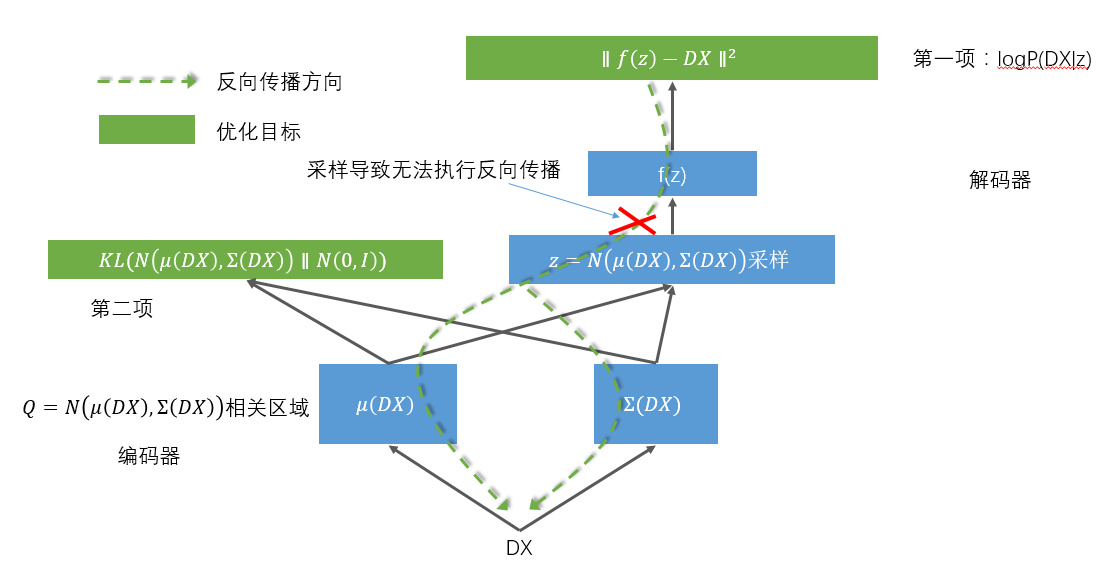
\includegraphics[width=12cm]{images/VAE_net_structure1.jpg}
            \caption{VAE网络结构示意图1}
            \label{fig:VAE网络结构示意图1}
            \end{figure}
            % \textcolor[rgb]{1 0 0}{todo:图片:VAE网络结构示意图1}
            \par
            \ding{173}对式(\ref{VAE的目标L})$L$中的第二项。由于$z$是采样而来的,$z\sim q(z|x) = N(\mu,\sigma^2)$,因而$L$不能关于$\phi \overset{\Delta}{=}(\mu,\sigma)$求导。如果$z$是其它操作(非采样操作,例如$z = (A+B)C$等),那么求导是没问题的。我们希望把采样($\sim$)这个随机操作变为某种确定性操作(例如$z = g_\phi(\cdot)$),可以进行如下确定性变换
            \begin{align*}
            z = g_\phi(\epsilon,x)
            \end{align*}
            其中:$\epsilon$是一个外来的随机变量,其概率分布为$p(\epsilon)$;$g_\phi(\cdot)$是一个关于参数$\phi$的向量值函数。
            \par
            假设$z_1,z_2,\dots,z_{n_h}$之间相互独立,则
            \begin{align*}
            \mathrm{d}z = \mathrm{d}z_1\mathrm{d}z_2\dots\mathrm{d}z_{n_h} = \prod_{i=1}^{n_h}\mathrm{d}z_i
            \end{align*}
            于是有
            \begin{align*}
            q_\phi(z|x)\mathrm{d}z \overset{\Delta}{=} q_\phi(z|x) \prod_{i=1}^{n_h}\mathrm{d}z_i = p(\epsilon) \mathrm{d} \epsilon
            \end{align*}
            于是
            \begin{align*}
            \int q_\phi(z|x) f(z)\mathrm{d}z = \int p(\epsilon) f(z)\mathrm{d}\epsilon
            \end{align*}
            将$z = g_\phi(\epsilon,x)$带入上式,有
            \begin{align*}
            \int q_\phi(z|x) f(z)\mathrm{d}z = \int p(\epsilon) f(g_\phi(\epsilon,x))\mathrm{d}\epsilon
            \end{align*}
            由此,我们就可对$L$(\ref{VAE的目标L})中的第二项$\int q_\phi(z|x)f(z)\mathrm{d}z$构建一个可微的估计量
            \begin{align*}
            \int q_\phi (z|x)f(z)\mathrm{d}z \approx \frac{1}{L}\sum_{l=1}^L f(g_\phi (x,\epsilon^l)) \quad \epsilon^l \sim p(\epsilon)
            \end{align*}
            现在可以对上式求导了。例:我们用高斯分布作为示例,设$z\sim p(z|x) = N(\mu,\sigma^2)$,一个有效的转化是$z = \mu + \sigma \epsilon$,其中:$\epsilon \sim N(0,1)$,因此
            \begin{align*}
            \mathbb{E} _{N(z;\mu,\sigma^2)}[f(z)] = \mathbb{E}_{N(\epsilon;0,1)}[f(\mu+\sigma \epsilon)] \approx \frac{1}{L} \sum_{l=1}^L f(\mu+\sigma \epsilon^l)
            \end{align*}
            其中:$\epsilon^l \sim N(0,1) $。对于上面的这种“确定性变换”,我们自然考虑:哪些$q_\phi(z|x)$可以进行可微转换$g_\phi(\cdot)$呢?并且有$\epsilon \sim p(\epsilon)$呢?关于这个问题,可以参考\cite{2014.Kingma}P5。
            \par
            上面的是在所有样本$x$上进行的,对于单一样本$x^k$,只要将$x$变为$x^k$即可。现在可以用MCMC来估计函数$f(z)$关于$q_\phi(z|x^k)$的期望了
            \begin{align*}
            \mathbb{E} _{q_\phi(z|x^k)}[f(z)] = \mathbb{E}_{p(\epsilon)}[f(g_\phi(\epsilon,x^k))] \approx \frac{1}{L} \sum_{l=1}^L f(g_\phi(\epsilon^l,x^k))
            \end{align*}
            其中:$\epsilon^l\sim p(\epsilon)$。我们将这种确定性转换技术应用到下界$L(\theta,\phi;x^k)$。\ding{172}考虑下界$L$的第一个写法
            \begin{align*}
            L(\theta,\phi;x^k)& = \mathbb{E}_{q_\phi(z|x^k)} \left[ \log p_\theta(x^k,z) - \log q_\phi(z|x^k) \right]\\
            & \approx \frac{1}{L} \sum_{l=1}^L \left[ \log p_\theta(x^k,z^l) - \log q_\phi (z^{k,l}|x^k) \right]
            \end{align*}
            其中:$z^{k,l} = g_\phi(\epsilon^{k,l},x^k)$,$\epsilon ^k \sim p(\epsilon)$。记此估计量为$\tilde{L}^A(\theta,\phi;x^k)$。\\
            \ding{173}考虑下界$L$的第二个写法
            \begin{align*}
            L(\theta,\phi;x^k) = - KL(q_\phi(z|x^k)||p_\theta(z|x^k)) + \mathbb{E}_{q_\phi(z|x^k)} \left[ \log p_\theta(x^k|z) \right]
            \end{align*}
            上式得$-KL$项在前面已经分析过了,可以对$\mu,\sigma$求导,但后面的积分项(期望值)不行,我们将确定性变换$z = g_\phi(\epsilon,x)$技术用上来,就变为
            \begin{align*}
            L(\theta,\phi;x^k) = -KL(q_\phi(z|x^k) || p_\theta(z|x^k))+ \frac{1}{L}\sum_{l=1}^L \log p_\theta(x^k|z^{k,l})
            \end{align*}
            其中:$z^{k,l} = g_\phi(\epsilon^{k,l},x^k)$,$\epsilon^l\sim p(\epsilon)$。我们记此估计量为$\tilde{L}^B(\theta,\phi;x^k)$。
            \par
            现在,$\tilde{L}^B(\theta,\phi;x^k)$和$\tilde{L}^A(\theta,\phi;x^k)$可以对$\phi$求导了。上面是单一样本$x^k$,对于批量样本而言,设$x^M$是从样本集中随机挑选的$M$个样本,则其估计量为
            \begin{align*}
            L(\theta,\phi;x^M) \approx \tilde{L}^M(\theta,\phi;x^M) = \frac{m}{M} \sum_{k=1}^M \tilde{L}(\theta,\phi;x^k)
            \end{align*}
            批量样本的SGVB算法如下(\ref{code:SGVB})
            \begin{algorithm}[htbp]
                \caption{SGVB for VAE}\label{code:SGVB}
                \begin{algorithmic}[1]
                    \State 初始化:$M$,$S = \{x^k\}_{k=1}^m$,MC链长$L =1$,初始参数$\theta^0,\phi^0$,迭代次数$t$,$t_{max}$,容许误差$\varepsilon$,学习率$\eta $。
                    \While {未达到终止条件 $t>t_{max}\ |\ ||\theta^{t+1},\phi^{t+1} - \theta^t,\phi^t||<\varepsilon$}
                        \State 随机挑选$M$个样本$x^M$;
                        \State $\epsilon \sim p(\epsilon)$;
                        \State $g \gets \nabla_{\theta,\phi}\tilde{L}^M(\theta,\phi;x^M,\epsilon)$;
                        \State $\theta,\phi \gets \theta,\phi + \eta g$
                    \EndWhile
                \end{algorithmic}
            \end{algorithm}
            \par
            仍然以$p_\theta(z|x^k) = N(0,I)$,$q_\phi(z|x^k)= N(\mu,\sigma^2)$为示例,经过确定性变化后,VAE的网络结构如图(\ref{fig:VAE网络结构示意图2})所示
            \begin{figure}[H]
            \centering
            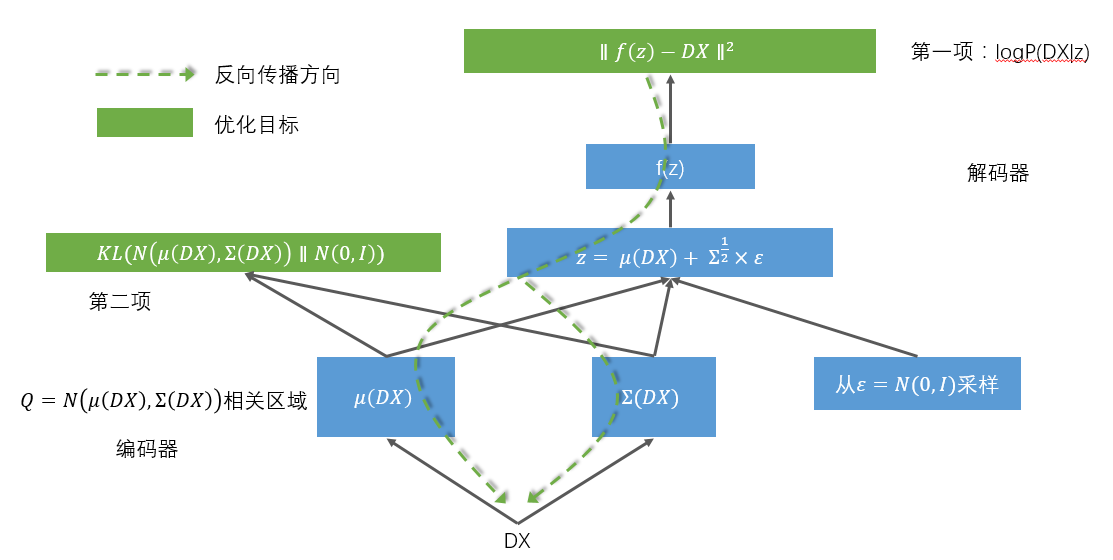
\includegraphics[width=12cm]{images/VAE_net_structure2.jpg}
            \caption{VAE网络结构示意图2}
            \label{fig:VAE网络结构示意图2}
            \end{figure}
            % \textcolor[rgb]{1  0 0}{todo:图片:VAE网络结构图2}

        \subsubsection{VAE的梳理}
            \par
            下面来捋一下VAE。假设$p_\theta(z|x^k)$为多元正态分布$N(0,I)$;如果样本为实值,则设$p_\theta(x|z)$为多维高斯分布,如果样本是01二值的,则设$p_\theta(x|z)$为多维二项分布。假设$q_\phi(z|x^k)$是多维高斯分布$N(\mu^k,\sigma^k{}^2)$,这里$\mu^k,\sigma^k$为向量,$\mu^k = (\mu_1^k,\mu_2^k,\dots,\mu_{n_h}^k)$。
            \par
            对于某一个样本$x^k$,将$x^k$输入到VAE网络中,通过编码器$f$,可以得到其均值向量和方差向量$\mu^k,\sigma^k$,于是,我们得到了$q_\phi(z|x^k)$
            \begin{align*}
            q_\phi(z|x^k) = N(z;x^k,\sigma^{k2}I)
            \end{align*}
            然后要在$q_\phi(z|x^k)$中选取$L$个样本,$z^{k,l} \sim q_\phi(z|x^k)$,为了使其可导,我们用确定性转化技术
            \begin{align*}
            z^{k,l} = g_\phi(x^k,\epsilon^l) = \mu^k+\sigma^k\odot \epsilon^l
            \end{align*}
            其中:$\epsilon^l \sim N(0,I)$;$\odot$是元素操作。于是,我们可以得到下界
            \begin{align*}
            L(\theta,\phi;x^k) = \frac{1}{2}\sum_{j=1}^{n_h} \left( 1+\log(\sigma_j^k)^2 - (\mu_j^k)^2 - (\sigma_j^k)^2 \right) + \frac{1}{L}\sum_{l=1}^L \log p_\theta(x^k|z^{k,l})
            \end{align*}
            关于$p_\theta(x^k|z)$的计算,可以用MLP来充当decoder:\ding{172}如果$x$是01二值的,则$p_\theta(x|z)$为多维伯努利分布,其MLP的结构如图(\ref{fig:MLP充当解码器示意图1})所示
            \begin{figure}[H]
            \centering
            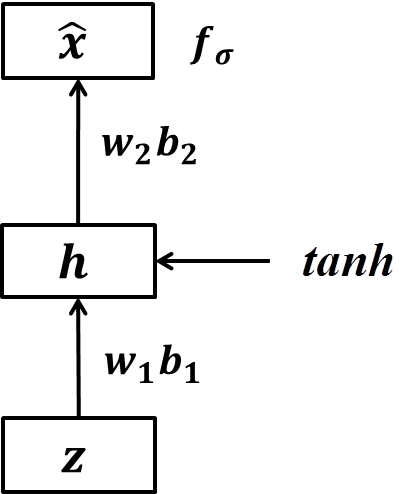
\includegraphics[height=3cm]{images/MLP_acts_as_decoder1.png}
            \caption{MLP充当解码器示意图1}
            \label{fig:MLP充当解码器示意图1}
            \end{figure}
            % \textcolor[rgb]{1 0 0}{todo:图片:MLP充当解码器示意图1}\\
            图(\ref{fig:MLP充当解码器示意图1})中的$\hat{x}$为
            \begin{align*}
            \hat{x} = f_\sigma (W_2\mathrm{tanh}(W_1z+b_1)+b_2)
            \end{align*}
            令$\theta \overset{\Delta}{=} (W_1,W_2,b_1,b_2)$,tanh和$f_\sigma$为传递函数,于是,得到样本的概率为
            \begin{align*}
            \log p_\theta(x|z) = \sum_{i=1}^m x_i \log \hat{x}_i + (1-\hat{x}_i)\log (1-\hat{x}_i)
            \end{align*}
            \ding{173}如果$x$不是01变量,而是实值变量,设$p_\theta(z|x)$为多维高斯分布。为多维伯努利分布,其MLP的结构如图(\ref{fig:MLP充当解码器示意图2})所示
            \begin{figure}[H]
            \centering
            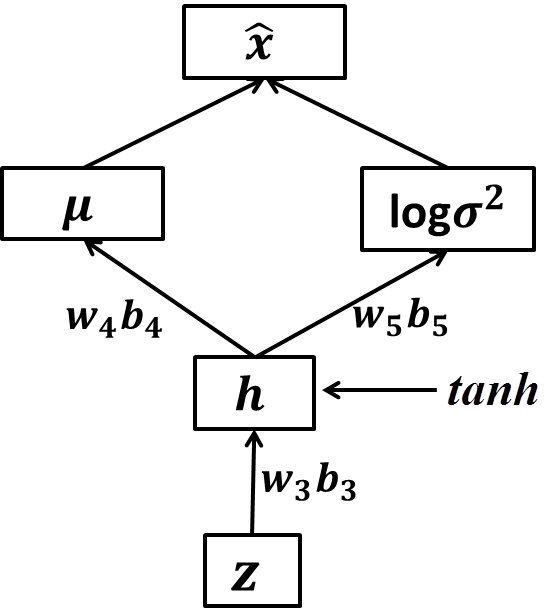
\includegraphics[height=3cm]{images/MLP_acts_as_decoder2.png}
            \caption{MLP充当解码器示意图2}
            \label{fig:MLP充当解码器示意图2}
            \end{figure}
            % \textcolor[rgb]{1 0 0}{todo:图片:MLP充当解码器示意图2}\\
            图(\ref{fig:MLP充当解码器示意图2})中的变量为
            \begin{align*}
            & h=\mathrm{tanh}(W_3z+b_3)\\
            & \mu=W_4h+b_4\\
            & \log \sigma^2 W_5h+b_5\\
            & \log p_\theta (x|z) = \log N(x;\mu,\sigma^2I)
            \end{align*}
            将\ding{172}或\ding{173}中的$\log_\theta p(x|z)$变为单一样本的情况,有
            \begin{align*}
            \log p_\theta (x^k|z^{k,l})
            \end{align*}
    \subsection{重要性加权自动编码器IWAE}
        \subsubsection{深层VAE}
            \par
            Importance Weighted Autoencoders是Burda等人于2015年提出的改进版的VAE。在介绍IWVAE之前,先来把VAE的层数加深。在前面的VAE中,只有一个随机层/隐含层$z$,现在,将随机层$z$加深到$I$层,即共有$I$个随机层,并且假设$p_\theta(z_i|z_{i+1})$为多维正态分布,于是
            \begin{align*}
            & p_\theta(z) = p_\theta(z_I) \prod_{i=1}^{I-1}p_\theta(z_i|z_{i+1}) = p_\theta(z_I) p_\theta(z_{I-1}|z_I) \dots p_\theta(z_1|z_2)\\
            & p_\theta(z_I) = N(z_I|0,I)\\
            & p_\theta(z_i|z_{i+1}) = N(z_i|\mu_i,\sigma_i^2)\\
            & p_\theta(x|z_1) = N(x|\mu(z_1),\sigma^2(z_1)) \quad \mathrm{or} \quad p_\theta(x|z_1) = B(z|\mu(z_1))
            \end{align*}
            其中:$\mu_i,\sigma_i$是向量。上面是解码过程(生成),下面,给出在编码过程中模型的条件分布情况,仍然假设$q_\phi(z_i|z_{i-1})$是高斯分布
            \begin{align*}
            & q(z|x) = q_\phi(z_1|x) \prod_{i=1}^Iq_\phi(z_i|z_{i-1})\\
            & q_\phi(z_1|x) = N(z_1|\mu(x),\sigma^2(x))\\
            & q_\phi(z_i|z_{i-1}) =N(z_i|\mu(z_{i-1}),\sigma^2(z_{i-1}))\quad i=2,3,\dots,I
            \end{align*}
            \par
            我们继续讨论目标函数(对数似然)的变分下界,由Jensen不等式,有
            \begin{align*}
            \log p(x) = \log \mathbb{E}_{q_\phi(z|x)} \left[ \frac{p(x,z)}{q_\phi(z|x)}  \right] \geqslant \mathbb{E}_{q_\phi(z|x)}\left[ \log \frac{p(x,z)}{q_\phi(z|x)} \right] = L(\theta,\phi;x)
            \end{align*}
            或者是
            \begin{align*}
            \log p(x) = KL(q_\phi(z|x)||p(z|x)) + L(\theta,\phi;x)
            \end{align*}
            \par
            将$L(\theta,\phi;x)$关于$\theta,\phi$求导,由于随机采样,导致导数不可求,我们采用确定性转化技术(reparameterization trick):原本的采样过程如图(\ref{fig:IWVAE随机采样})所示
            \begin{figure}[H]
            \centering
            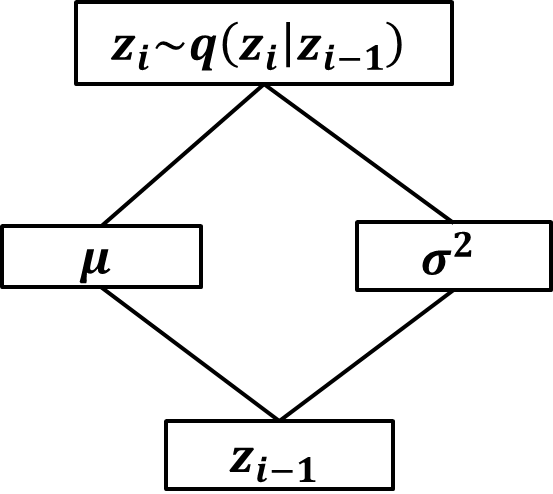
\includegraphics[height=3cm]{images/IWVAE_random_sampling.jpg}
            \caption{IWVAE随机采样}
            \label{fig:IWVAE随机采样}
            \end{figure}
            % \textcolor[rgb]{1 0 0}{todo:图片:IWVAE随机采样}\\
            \begin{align*}
            z_i^l \sim q_\phi(z_i|z_{i-1}) = N(z_i|\mu(z_{i-1}),\sigma^2(z_{i-1}))
            \end{align*}
            其中:$l=1,2,\dots,L$,$L$表示第$i$层$z_i$的采样数。经过确定性转化,采样过程如图(\ref{fig:IWVAE确定性采样})所示
            \begin{figure}[H]
            \centering
            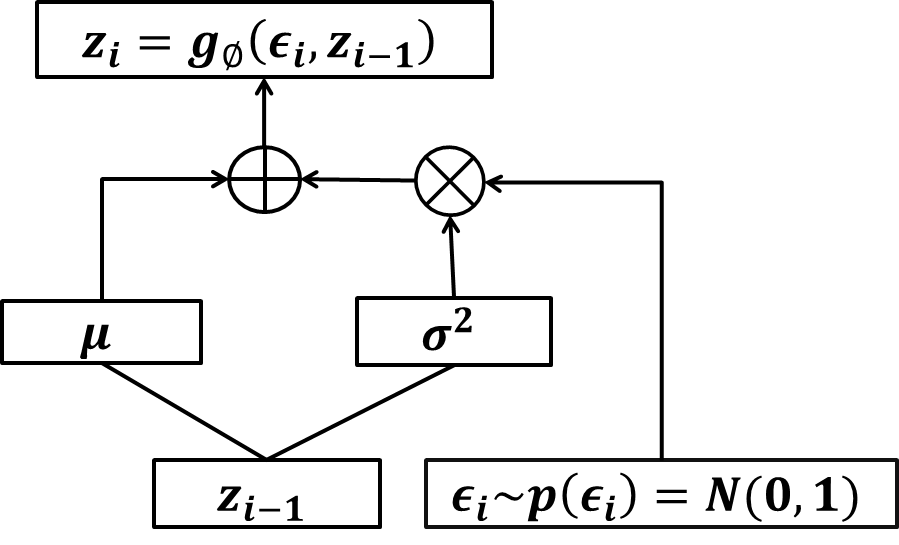
\includegraphics[height=3cm]{images/IWVAE_Deterministic_sampling.jpg}
            \caption{IWVAE确定性采样}
            \label{fig:IWVAE确定性采样}
            \end{figure}
            % \textcolor[rgb]{1 0 0}{todo:图片:IWVAE确定性采样}\\
            \begin{align*}
            z_i = g_\phi(\epsilon_i,z_{i-1}) = \mu_i(z_{i-1}) + \sigma(z_{i-1})\epsilon_i\\
            z_i^l = g_\phi(\epsilon_i^l,z_{i-1}) = \mu_i(z_{i-1}) + \sigma(z_{i-1}) \odot\epsilon_i
            \end{align*}
            其中:$\epsilon_i^l \sim p(\epsilon_i),i=1,2,\dots,I$,$\epsilon = (\epsilon_1,\epsilon_2,\dots,\epsilon_I)$,每个随机层$z_i$都有一个辅助的随机量$\epsilon_i\sim p(\epsilon_i)$,并且在$\epsilon_i$上进行$L$次采样,$z_i^l = g_\phi(\epsilon_i^l,z_{i-1})$
            \par
            使用确定性转化技术后,$L(\theta,\phi;x)$关于$\phi$可导,有
            \begin{align*}
            \frac{\partial }{\partial \phi} & = \nabla_\phi \mathbb{E} _{q_\phi(z|x)} \left[ \log \frac{p(x,z)}{q_\phi(z|x)} \right]\\
            & = \nabla_\phi \mathbb{E} _{z\sim q_\phi(z|x)} \left[ \log\frac{p(x,z)}{q_\phi(z|x)} \right]\\
            & = \nabla_\phi \mathbb{E}_{\epsilon\sim N(0,I)} \left[ \log\frac{p(x,g_\phi(\epsilon,x))}{q_\phi(g_\phi(\epsilon,x)|x)} \right]\\
            & = \mathbb{E} _{\epsilon_1,\epsilon_2,\dots,\epsilon_I \sim N(0,I)} \nabla_\phi \log\frac {p}{q_\phi}
            \end{align*}
        \subsubsection{加权VAE}
        \par
        IWVAE和VAE有相同的网络结构,不同的是,IWVAE构建了一个加权的$\log p(x)$下界。VAE的变分下界为
        \begin{align*}
        \mathcal{L}(\theta,\phi;x) = \mathbb{E}_{z\sim q_\phi(z|x)} \left[ \log \frac{p(x,z)}{q_\phi(z|x)} \right]
        \end{align*}
        IWVAE的变分下界为
        \begin{align*}
        \mathcal{L}_L(\theta,\phi;x) =\mathbb{E}_{z^1,\dots,z^L \sim q_\phi(z|x)} \left[ \log \frac 1 L \sum_{l=1}^L \frac{p(x,z^l)}{q(z^l|x)} \right]
        \end{align*}
        其中:$z^1,z^2,\dots,z^L$是从识别模型中采取的相互独立的样本,$z^1,z^2,\dots,z^L\sim q_\phi(z|x)$。我们记
        \begin{align*}
        w_l = \frac{p(x,z^l)}{q_\phi(z^l|x)}
        \end{align*}
        于是下界$\mathcal{L}_L(\theta,\phi;x)$可以写为
        \begin{align*}
        \mathcal{L}_L = \mathbb{E} \left[\log \frac{1}{L} \sum_{l=1}^L w_l \right] \leqslant \log \mathbb{E}\left[ \frac{1}{L}\sum_{i=1}^Lw_l \right] = \log p(x)
        \end{align*}
        \par
        对上面的加权目标$\mathcal{L}_L$,我们有下面结论\cite{2016.Burda}(Approdix A):
        \begin{align*}
        \log p(x) \geqslant \mathcal{L}_{L+1} \geqslant \mathcal{L}_L \quad \forall L>0
        \end{align*}
        此外,如果$\frac{p(z|x)}{q_\phi(z|x)}$是有界的,那么,当$L\rightarrow \infty$时,有$L_L \rightarrow \log p(x)$。这个下界$\mathcal{L}_L$可以用MC方法来近似。我们从识别模型中抽取$L$个样本,$z^l,l=1,2,\dots,L$,然后再平均它们的重要性权重。有人可能会担心这个估计量有较大的方差,关于方差的计算,可以参考\cite{2016.Burda}(Approdix B)。
        \par
        下面,我们来计算下界$\mathcal{L}_L$关于$\theta,\phi$的导数。像VAE中分析的那样,我们仍然采用确定性转化技术,有
        \begin{align*}
        \frac{\partial \mathcal{L}_L(\theta,\phi;x)}{\partial \theta} & = \nabla_\theta \mathbb{E}_{z^1,z^2,\dots,z^L\sim q_\phi(z|x)} \left[ \log \frac{1}{L}\sum_{l=1}^Lw_l \right]\\
        & =\nabla_\theta \mathbb{E}_{\epsilon^1,\epsilon^2,\dots,\epsilon^L\sim N(0,I)} \left[ \log\frac{1}{L}\sum_{l=1}^L w \left( x,g_\phi(\epsilon^l,x;\theta);\theta \right)  \right]\\
        & =\mathbb{E}_{\epsilon^1,\epsilon^2,\dots,\epsilon^L\sim N(0,I)}  \left[\nabla_\theta  \log\frac{1}{L}\sum_{l=1}^L w \left( x,g_\phi(\epsilon^l,x;\theta);\theta \right)  \right]\\
       &  =\mathbb{E}_{\epsilon^1,\epsilon^2,\dots,\epsilon^L\sim N(0,I)}  \left[ \sum_{l=1}^L \tilde{w}_L\nabla_\theta\log w \left( x,g_\phi(\epsilon^l,x;\theta);\theta \right)  \right]
        \end{align*}
        其中:$\epsilon^1,\epsilon^2,\dots,\epsilon^L$是去了$L$次样本;$\epsilon^l = (\epsilon_1^l,\epsilon_2^l,\dots,\epsilon_I^l)$表示共有$I$个特征层$z$。$w_L = w(x,g(x,\epsilon^l;\theta);\theta)$是权重函数;$\tilde{w}_l = \frac{w_l}{\sum_l w_l}$是归一化权重。特别的,当$L = 1$时,$\tilde{w}_1 =1$。
        \begin{align*}
        \nabla_\theta\log w \left( x,g_\phi(\epsilon^l,x;\theta);\theta \right) &= \nabla_\theta \log p(x,g_\phi(x,\epsilon^l;\theta);\theta) \\
        &\quad - \nabla_\theta \log q_\phi (g_\phi(x,\epsilon^l;\theta)|x;\theta)
        \end{align*}
        上式中等号右边第一项鼓励生成模型(decoder)分配高的概率给每一个$z_i$(在给定$z_{i+1}$后),它同时也鼓励识别模型(encoder)调整随机层$q_\phi(z|x)$来做更好的预测。
        \par
        关于VAE的改进,还可以参考:Laddder VariationalAutoEncoder\cite{2016.Casper};2016.Rolfe\cite{2016.Rolfe}的Discrete Variational AutoEncoder;以及2016.Suwon\cite{2016.Suwon}。
    \subsection{随机生成网络GSN}
        \par
        Generative Stochastic Networks(GSN)是Bengio于2013年提出的一种生成网络,是去噪自动编码器DAE的推广。先回顾一下DAE:我们有样本数据$X=\{x^k\}_{k=1}^m$,$X\in R^{m\times n}/\{0,1\}^{m\times n}$,设AE网络有输入层、隐含层/特征层和输出层3层,要求$p(x)$,即样本的分布。这个问题本质是一个密度函数的估计(拟合)问题,如果对$p(x)$的分布形式进行假设,比如我们假设$p(x)$是多元高斯分布,那么,只要求多元高斯中的参数$\theta$即可。DAE在原样本中加入噪声$\varepsilon$,使原始样本数据$x$变为$\tilde{x} = x+\varepsilon$,然后用$\tilde{x}$进行训练。我们设含噪声的随机变量$\tilde{x}$的分布为$C(\tilde{x}|x)$,则$\tilde{x}\sim C(\tilde{x}|x)$,训练过程为
        \begin{align*}
        & h=f_{\theta_1}(\tilde{x})\\
        & \hat{x}= g_{\theta_2}(h)
        \end{align*}
        其中:$\theta \overset{\Delta}{= } (\theta_1,\theta_2)$,$h$为特征层/隐含层。一般的目标可以是离差平方和或者极大似然函数。
        \par
        原来的对$p(x)$的估计是一个无监督问题,而我们可以将DAE视为有监督问题,就像给定$\tilde{x}$求$x$一样。我们称$\tilde{x}$是坏样本(含噪声样本/损坏样本),对于同一个样本$x^k$,可以对其添加不同的噪声,形成不同的坏样本。如果DAE网络训练结束后($\theta$求解结束),对于一个已经损坏的样本$\tilde{x}^*$,我们就可以给出它的估计$\hat{x}^*$。具体的对于图像识别而言,给一张含糊不清的数字图片$\tilde{x}^*$,如图(\ref{fig:DAE做图像判别的示意图})
            \begin{figure}[H]
            \centering
            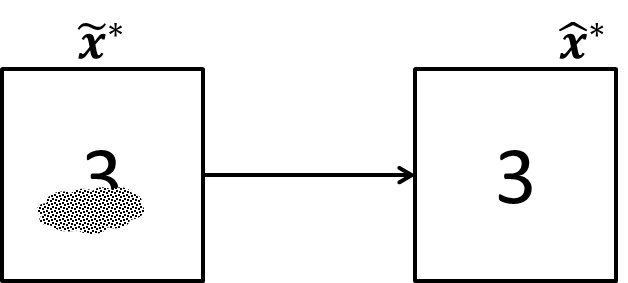
\includegraphics[height=3cm]{images/DAE_for_Image_discrimination.jpg}
            \caption{DAE做图像判别的示意图}
            \label{fig:DAE做图像判别的示意图}
            \end{figure}
        % \textcolor[rgb]{1 0 0}{todo:图片:DAE做图像判别的示意图}\\
        通过DAE我们就能给出$\hat{x}^* = 3$的概率。一定要注意$p_\theta(x|\tilde{x})$是一个识别问题,像回归一样$y|x\sim N$。上面遗留的问题是:在网络参数$\theta$训练完成后,如何识别坏样本,并且这个坏样本的估计量$\hat{x}^*$的统计性质如何?对于DAE,还有一个问题,我们说DAE网络中包含了样本$x$的信息,整个样本$x$的密度函数已经估计出来了,即$p(\hat{x}|\tilde{x)}$,那如何从这个分布中采样呢?
        \par
        在回答上面两个问题之前,先来介绍一个新的网络GSN。我们说GSN是DAE的推广,DAE是在$x$中添加了噪声,自然想能否在$h$中也添加噪声,形成$\tilde{h}$?GSN的网络结构图如图(\ref{fig:GSN的网络结构示意图})所示
                \begin{figure}[H]
                  \centering
                  \begin{varwidth}[t]{\textwidth}
                    \vspace{0pt}
                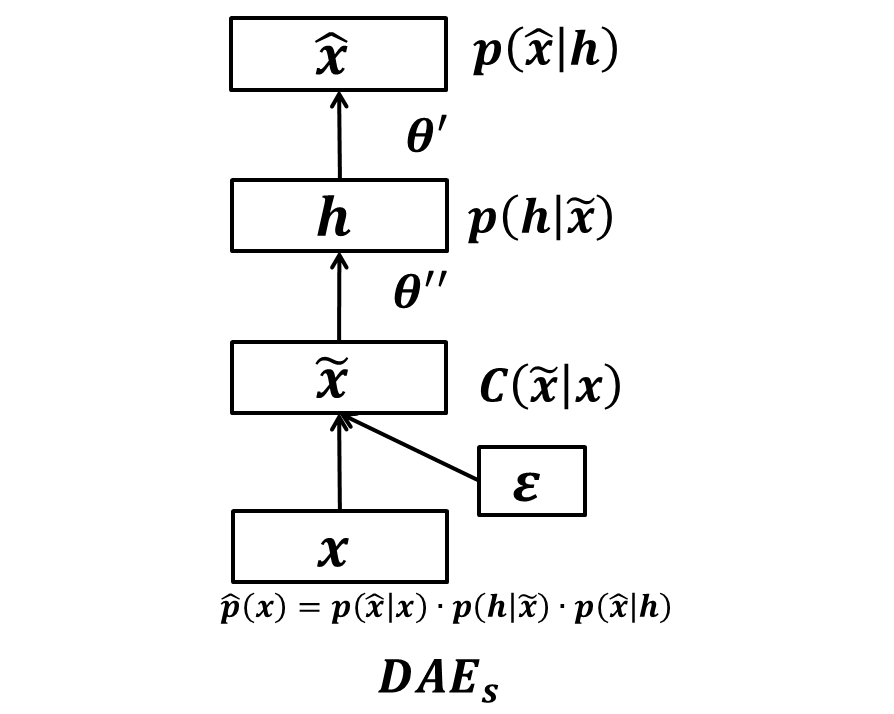
\includegraphics[height=4cm]{images/GSN_net_structure1.jpg}
                  \end{varwidth}
                  \qquad
                  \begin{varwidth}[t]{\textwidth}
                    \vspace{0pt}
                    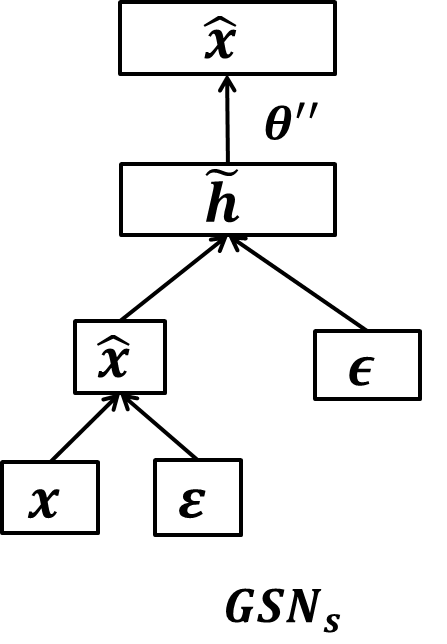
\includegraphics[height=4cm]{images/GSN_net_structure2.jpg}
                  \end{varwidth}
            \caption{GSN的网络结构示意图}
            \label{fig:GSN的网络结构示意图}
                \end{figure}
        % \textcolor[rgb]{ 1 0 0}{todo:图片:GSN的网络结构示意图}\\
        在$x$部分增加噪声$\varepsilon$,在$h$部分增加噪声$\epsilon$。问题是:GSN的求导可以进行吗?可以看到,GSN就和VAE的确定性转换技术一样,所以GAN是可以直接求导的。
        \par
        下面,来处理上面遗留的两个问题:\ding{172}损坏样本的估计;\ding{173}如何采样。先来处理第二个问题,前面介绍了各种各样的自动编码器,自动编码器内存放着数据$x$的分布,现在要从这个分布中采样。可以尝试采用前面介绍的MCMC采样。Bengio(2013)给出了一个从参数分布$p_\theta(x)$中采样的方法:通过运行马尔科夫链交替增加噪声到近似的真实分布$p(x|\tilde{x})$当中。文中表明,如果一个学习后的参数分布$p_\theta(x|\tilde{x})$接近真实分布$p(x|\tilde{x})$,在一些优良的条件下,运行一段马氏链后,平稳分布$\pi(x)$会收敛到真实分布$p(x)$。假设我们已经训练好了AE网络,从当前样本$x$开始($x$可以是一个样本,也可以是一批样本),则由AE形成的马氏链为
        \begin{enumerate}
        \item 从当前状态$x$开始,向$x$中注入噪声$\varepsilon$,有$\tilde{x}\sim C(\tilde{x}|x)$;
        \item 将$\tilde{x}$编码。$h = f(\tilde{x})$;
        \item 解码$h$。$\hat{x} = g(h)$,且$p(x|\hat{x} =g(h)) = p(x|\tilde{x})$;
        \item 从$p(x|\hat{x}) = p(x|\tilde{x})$中采样一个状态$x$。
        \end{enumerate}
        \par
        Bengio(2014)表明,如果自动编码器$p(\hat{x}|\tilde{x})$是真实分布$p(x|\tilde{x})$的一致估计量,则上述马尔科夫链平稳分布$\pi(x)$是$x$分布$p(x)$的一致估计量(虽然是隐含的)。
        \par
        形式上,用$p_{\theta_n}(\hat{x}|\tilde{x})$表示经过$n$次训练的DAE,他表示给定$\tilde{x}\sim C(\tilde{x}|x)$后,$x$的概率分布。这个估计量$p_{\theta_n}(\hat{x}|\tilde{x})$定义了一个马尔科夫链$T_n$:不断交替采样$\tilde{x}\in C(\tilde{x}|x)$,$x \sim p_\theta(\hat{x}|\tilde{x})$。我们设$\pi_n$是$T_n$的平稳分布,则有如下定理
        \begin{theorem}
        如果$p_{\theta_n}(\hat{x}|\tilde{x})$是真实分布$p(x|\tilde{x})$的一致估计量,并且$T_n$是一个马尔科夫链,则当$n\rightarrow \infty$时,平稳分布$\pi_n(x)$收敛到数据分布$p(x)$。
        \end{theorem}
        并且,为了使上述定理可行,要求$T_n$具有遍历性。DAE的采样示意图如图(\ref{fig:DAE采样示意图})所示
            \begin{figure}[H]
            \centering
            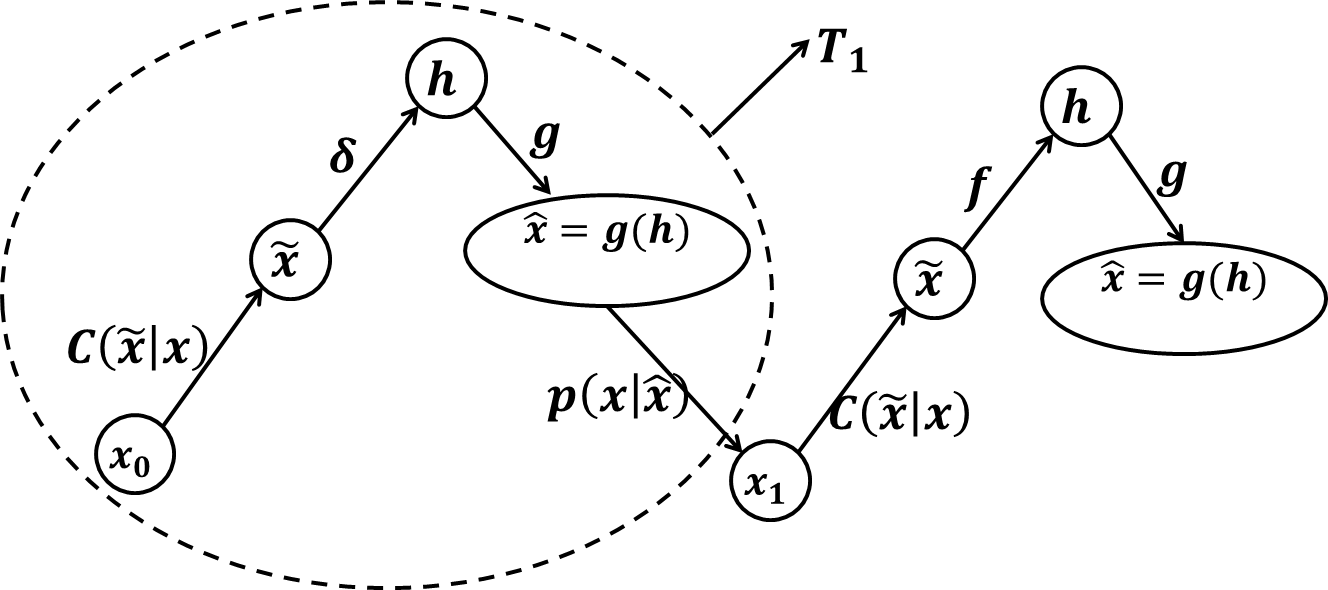
\includegraphics[height=3cm]{images/DAE_sampling.jpg}
            \caption{DAE采样示意图}
            \label{fig:DAE采样示意图}
            \end{figure}
        % \textcolor[rgb]{1 0 0}{todo:图片:DAE采样示意图}\\
        图(\ref{fig:DAE采样示意图})中:马尔科夫链的每个步骤与训练好的DAE相关联,每个步骤包括:(a)通过损坏过程$C$向状态$x$中注入噪声$\varepsilon$产生$\tilde{x}$;(b)用函数$f$进行编码,产生$h = f(\tilde{x})$;(c)用函数$g$进行解码,产生用于重构分布的参数$w\overset{\Delta}{=}g(h)$,在一般的平方重构误差下,$w = \hat{x} = g(h)$;(d)给定$w$,从重构分布$p(x|w)$采样新状态$x$。
        \par
        上面给出了DAE的马尔科夫链$x_t$,$\tilde{x}\sim C(\tilde{x}|x_t)$,$x_{t+1} \sim p_\theta (x|\tilde{x}_t)$。下面给出GSN的马尔科夫链。我们将GSN中的$x$和$h$都做为马尔科夫链的状态,有
        \begin{align*}
        & h_{t+1}\sim p_{\theta_1} (h|h_t,x_t) \\
        & x_{t+1}\sim p_{\theta_2} (x|h_{t+1})
        \end{align*}
        定义
        \begin{align*}
        h_{t+1} = f_{\theta_1}(x_t,\epsilon_t,h_t)
        \end{align*}
        其中:$\epsilon_t$是引入到隐含层的噪声。可以看出DAE是GSN的特殊情况。
        \begin{theorem}
        设训练样本$x\sim p(x)$,噪声$\epsilon\sim p(\epsilon)$,并且在隐含层$h$中添加噪声
        \begin{align*}
        h_t = f_{\theta_1}(x_{t-1},\epsilon_{t-1},h_{t-1})
        \end{align*}
        考虑模型$p_{\theta_2}(x|f_{\theta_1}(x,\epsilon_{t-1},h_{t-1}))$:对一个给定的$\theta_1$,$p_{\theta_2}(x|h)$是一个$p(x|h)$的估计量。设马尔科夫链的平稳分布$\pi_n(x,h)$的边缘分布为$\pi_n(x)$,当训练次数$n\rightarrow \infty$时,$\pi_n(x)\rightarrow p(x)$。
        \end{theorem}
        \par
        GSN的马尔科夫链如图(\ref{fig:GSN马尔科夫链示意图})所示
            \begin{figure}[H]
            \centering
            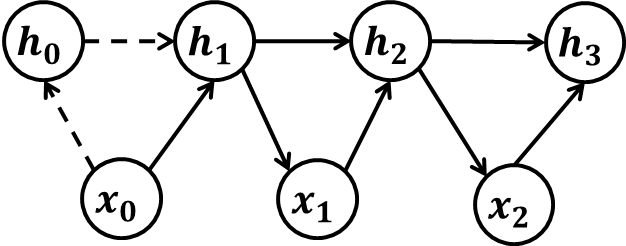
\includegraphics[height=3cm]{images/GSN_Markov_chain_diagram.jpg}
            \caption{GSN马尔科夫链示意图}
            \label{fig:GSN马尔科夫链示意图}
            \end{figure}
        % \textcolor[rgb]{1 0 0}{todo:图片:GSN马尔科夫链示意图}\\
        % \textcolor[rgb]{1 0 0}{引入2015.Alain.G Bengio 的Fig5的右图}
        \begin{theorem}
        设$(h_t,x_t)_{t=0}^\infty$是上图定义的马尔科夫链,假设这个马尔科夫链有平稳分布$\pi(x,h)$,并且对于每一个值$(x,h)$,如果
        \begin{enumerate}
        \item 所有的$p(x_t=x|h_t=h) = g(x|h)$有相同的密度,$t \geqslant 1$;
        \item 所有的$p(h_{t+1}=h|h_t=h',x_t=x) = f(h|h',x)$有相同的密度,$t \geqslant0 $;
        \item $p(h_0=h|x_0=x) = p(h_1=h|x_0=x)$;
        \item $p(x_1=x|h_1=h) = p(x_0=x|h_1=h)$
        \end{enumerate}
        那么,对于每个值$(x,h)$,我们会有
        \begin{enumerate}
        \item $p(x_0=x|h_0=h) = g(x|h)$;
        \item $p(x_0=x|h_t=t)=p(x_0=x,h_0=h$,$t \geqslant 0$;
        \item 平稳分布$\pi(x,h)$的边缘分布$\pi(x) = p(x_0 = x)$
        \end{enumerate}
        \end{theorem}
        上述结论表明:马尔科夫链的样本与$x_0$来自相同的分布。
    \subsection{beta - VAE}
        TODO: 待补充。。。
    \subsection{MATLAB应用实例}
        \subsubsection{MATLAB自带工具}
        \par
        MATLAB自带的自动编码器命令如表(\ref{tab:Autoencoders命令})所示
        \begin{table}[htbp]
          \caption{Autoencoders命令}
          \label{tab:Autoencoders命令}
          \centering
          \begin{tabular}{l|l}
          \toprule
          命令  & 说明 \\
          \midrule
          Autoencoder &  Autoencoder class\\
          trainAutoencoder & 训练自动编码器\\
          trainSoftmaxLayer &  Train a softmax layer for classification\\
          decode & Decode encoded data\\
          encode & Encode input data\\
          generateFunction & Generate a MATLAB function to run the autoencoder\\
          generateSimulink & Generate a Simulink model for the autoencoder\\
          network  & Convert(转变) Autoencoder object into network object\\
          plotWeights &  Plot a visualization of the weights for the encoder of an autoencoder\\
          predict &  Reconstruct(重建) the inputs using trained autoencoder\\
          stack &  Stack encoders from several autoencoders together\\
          view & View autoencoder\\
          \bottomrule
          \end{tabular}
        \end{table}
        \par
        % MATLAB构建AE的示例:
        % \begin{lstlisting}[language = Matlab]
        % %% 图像分类的Stacked Autoencoders(SAE)
        % % https://cn.mathworks.com/help/nnet/examples/training-a-deep-neural-network-for-digit-classification.html
        % %% 加载数据
        % % Load the training data into memory
        % [xTrainImages,tTrain] = digitTrainCellArrayData;
        % %% TRAIN
        % %展示一些训练图片
        % clf
        % for i = 1:20
        %     subplot(4,5,i);
        %     imshow(xTrainImages{i});
        % end
        % % Training the first autoencoder
        % rng('default')
        % hiddenSize1 = 100;
        % autoenc1 = trainAutoencoder(xTrainImages,hiddenSize1, ...
        %     'MaxEpochs',400, ...
        %     'L2WeightRegularization',0.004, ...
        %     'SparsityRegularization',4, ...
        %     'SparsityProportion',0.15, ...
        %     'ScaleData', false);
        % view(autoenc1)
        % figure()
        % plotWeights(autoenc1);
        % feat1 = encode(autoenc1,xTrainImages);
        % % Training the second autoencoder
        % hiddenSize2 = 50;
        % autoenc2 = trainAutoencoder(feat1,hiddenSize2, ...
        %     'MaxEpochs',100, ...
        %     'L2WeightRegularization',0.002, ...
        %     'SparsityRegularization',4, ...
        %     'SparsityProportion',0.1, ...
        %     'ScaleData', false);
        % view(autoenc2)
        % feat2 = encode(autoenc2,feat1);
        % % Training the final softmax layer
        % softnet = trainSoftmaxLayer(feat2,tTrain,'MaxEpochs',400);
        % view(softnet)
        % % Forming a stacked neural network
        % view(autoenc1)
        % view(autoenc2)
        % view(softnet)
        % deepnet = stack(autoenc1,autoenc2,softnet);
        % view(deepnet)
        % % Get the number of pixels in each image
        % imageWidth = 28;
        % imageHeight = 28;
        % inputSize = imageWidth*imageHeight;
        % %% TEST
        % % Load the test images
        % [xTestImages,tTest] = digitTestCellArrayData;
        % % Turn the test images into vectors and put them in a matrix
        % xTest = zeros(inputSize,numel(xTestImages));
        % for i = 1:numel(xTestImages)
        %     xTest(:,i) = xTestImages{i}(:);
        % end
        % y = deepnet(xTest);
        % plotconfusion(tTest,y);
        % %% Fine tuning the deep neural network
        % % Turn the training images into vectors and put them in a matrix
        % xTrain = zeros(inputSize,numel(xTrainImages));
        % for i = 1:numel(xTrainImages)
        %     xTrain(:,i) = xTrainImages{i}(:);
        % end
        % % Perform fine tuning
        % deepnet = train(deepnet,xTrain,tTrain);
        % y = deepnet(xTest);
        % plotconfusion(tTest,y);
        % \end{lstlisting}

\section{卷积神经网络CNN}
    \subsection{基础卷积神经网络CNN}
        \par
        回忆之前提到过的网络模型,无论是MLP、Hopfield、SMO、BM、DBM、AE、VAE和GSN等,这些网络模型的输入层都是向量输入,即$x^k = (x^k_1,x_2^k,\dots,x_n^k)$,即便是批量或者全批量,也是以向量为样本的。整个样本的数据结构如图(\ref{fig:向量样本的数据示意图})所示
            \begin{figure}[H]
            \centering
            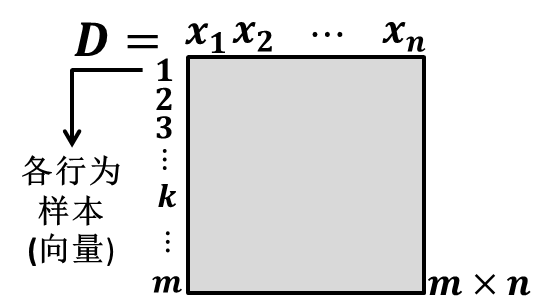
\includegraphics[height=3cm]{images/Vector_sample_of_the_data.jpg}
            \caption{向量样本的数据示意图}
            \label{fig:向量样本的数据示意图}
            \end{figure}
        % \textcolor[rgb]{1  0 0}{todo:图片:向量样本的数据示意图}\\
        也就是说,网络输入的样本$x^k$要是一个向量,比如,对于一个图像分类问题,要先将具体的图像样本(矩阵)变为向量,然后将向量输入到网络进行分类。自然会想,能不能把图像(矩阵)直接输入到网络中,因为对于图像处理而言,我们的样本就是一个个的图像矩阵。为此,要开发一个以矩阵为输入的神经网络(以及一些矩阵对矩阵的操作)。并且注意到如果图像是批量或者全批量样本,则是一个3维矩阵(张量)。
        \par
        幸运的是,我们已经有了这样的网络。下面要介绍的CNN网络就是一个以矩阵为样本的前馈网络(如果将CNN视为MLP的矩阵推广,那么Hopfield等网络能否推广到矩阵样本?)。如前面的神经网络一样,先来介绍CNN的网络结构,再介绍它的学习方法。
        \par
        1962年,Hubel和Wiesel通过对猫视觉皮层神经元的的研究,提出了感知野(receptive field)的概念;1980年,日本学者K.Fukushima提出了神经认知机,这也是第一代卷积神经网络;1989年,加拿大教授Yann LeCun提出了卷积神经网络(Convolution Neural Networks,CNN);2012年,深度学习大牛,DBN、DBM的开发者Hinton教授带领2个学生,采用更深的CNN在Image Net问题上取得了当时最好的结果,虽然这一结果之后一直被刷新,但CNN带来的视觉革命是不容忽视的。
        \subsubsection{CNN网络结构}
            \par
            假设有一个带标签的图像集/样本集$S = \{x^k,y^k\}_{k=1}^m$,$x^k$是一个图像矩阵,$y^k$是图像$x^k$的分类标签值。为了简便,我们将$x^k$视为$n\times n$方阵,$x^k\in R^{n\times n}/\{0,1\}^{n\times n}$,假设分类任务共有$c$类,则$y^k\in \{1,2,\dots,c\}$。现在,我们来看对于一个图片$x^k$而言,CNN的处理方式(前向传播),其处理流程如图(\ref{fig:CNN网络结构示意图})所示
            \begin{figure}[H]
            \centering
            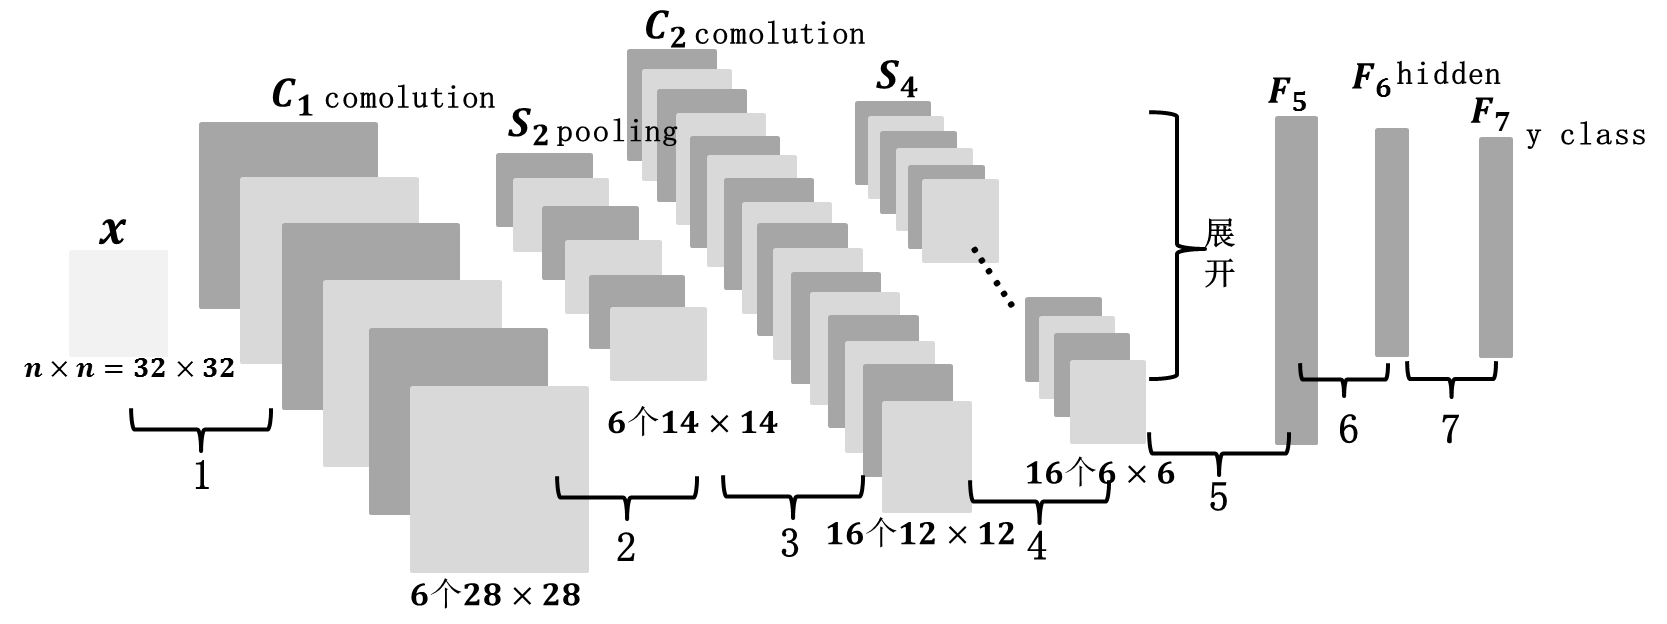
\includegraphics[height=5cm]{images/CNN_net_structure.jpg}
            \caption{CNN网络结构示意图}
            \label{fig:CNN网络结构示意图}
            \end{figure}
            % \textcolor[rgb]{1 0 0}{todo:图片:CNN网络结构示意图}
            \par
            这里给出的CNN网络结构(\ref{fig:CNN网络结构示意图})共有7个网络层。当然,我们可以继续加深网络,但是太深的CNN在反向传播过程中会出现误差消失/梯度消失的现象,具体而言,当我们从$F_1$层开始向$C_1$层传播,到了$C_1$层时,各$\theta$所分担的误差会非常小。在上面的7层CNN中,$C_1,S_2,C_3,S_4$都是为了从$x^k$中提取/获取特征,$F_5,F_6,F_7$是一个一般的BP神经网络(其它分类器亦可)。下面,我们来介绍每一步(每一层)的操作。\\
            $1\clubsuit$:对$C_1$层而言,输入为$32\times 32$大小的样本图片$x \overset{\Delta}{=}x^k$,输出为$6$个矩阵。并且,这6个矩阵的大小为$28\times 28$,与原矩阵$32\times 32$不一样,那么$1\clubsuit$是如何操作的才能产生这种结果呢?
            \par
            $1\clubsuit$过程是卷积过程(Colution),主要是利用卷积核(权重矩阵$w$,待求)来进行操作的。为了方便,我们设被卷积的图像$a$的大小为$5\times 5$,卷积核$w$大小为$3\times 3$,输出矩阵为$c$,则$a$到$c$的卷积过程如图(\ref{fig:卷积过程示意图})所示
            \begin{figure}[H]
            \centering
            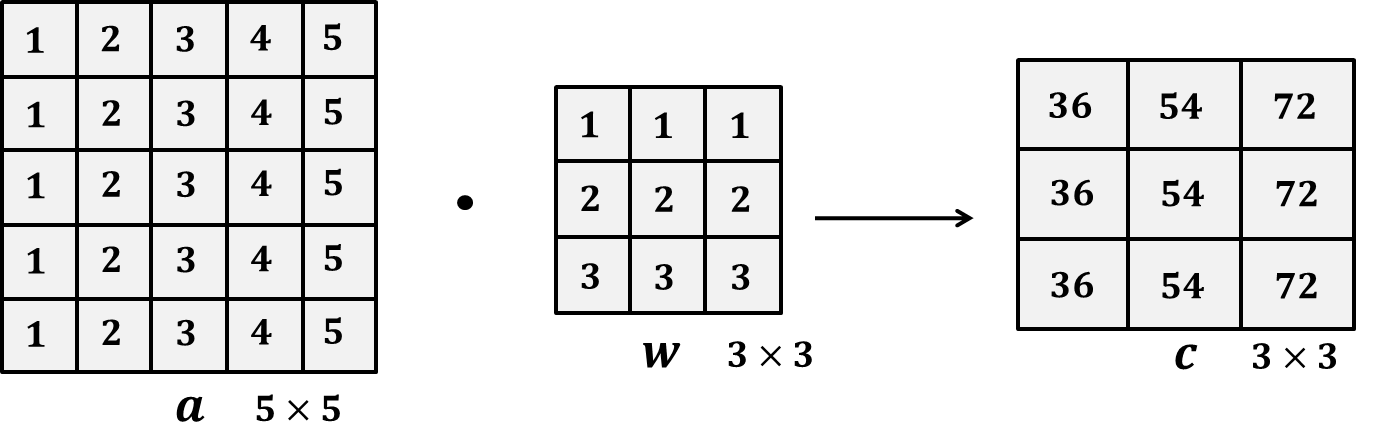
\includegraphics[height=3cm]{images/Colution.jpg}
            \caption{卷积过程示意图}
            \label{fig:卷积过程示意图}
            \end{figure}
            % \textcolor[rgb]{1 0 0}{todo:图片:卷积过程示意图}\\
            用$w$从$a$的左上角开始,找到同样大小的$3\times 3$局部矩阵,2个矩阵($w$和$a$的局部矩阵)对应元素相乘相加(卷积操作),得到36;之后,再把$w$一个点一个点的向右移动,卷积形成54和72;再将$w$向下移动,以形成其它的卷积值。可以计算,如果$a$是$m\times n$大小,$w$是$mx\times my$大小,则卷积后的$c$是$my\times ny$大小,其中:$my = m-mx+1,ny= n-nx+1$。你可能会有以下问题:
            \begin{enumerate}
            \item 是否要求输入图像$x$是01值?不限制;
            \item 是否要求输入图像$x$是方阵$n\times n$?不限制,但最好是;
            \item 为什么输入一张图片,结果卷积出来了6张图片?因为有6个卷积核$w_1,w_2,\dots,w_6$,并且注意:其实多个矩阵(map)可以公用一个卷积核,卷积之后结果相加,形成一个输出。
            \end{enumerate}
            $2\clubsuit$:$C_1$到$S_2$。对$S_2$而言,输入为6张图,输出为6张图,只不过大小从输入的$28\times 28$变为了$14\times 14$。那么,这6张图在$2\clubsuit$处都经历了什么?$S_2$层是一个池化过程/采样过程,从其名称“采样”可以看出,这是一个降维操作,以降低参数个数。该过程有2种常见的采样方法:一种是均值池化mean pooling;一种是最大池化max pooling。相对常用的是max pooling。我们用一个$28\times 28$的矩阵来演示池化过程,如图(\ref{fig:池化过程示意图})所示
            \begin{figure}[H]
            \centering
            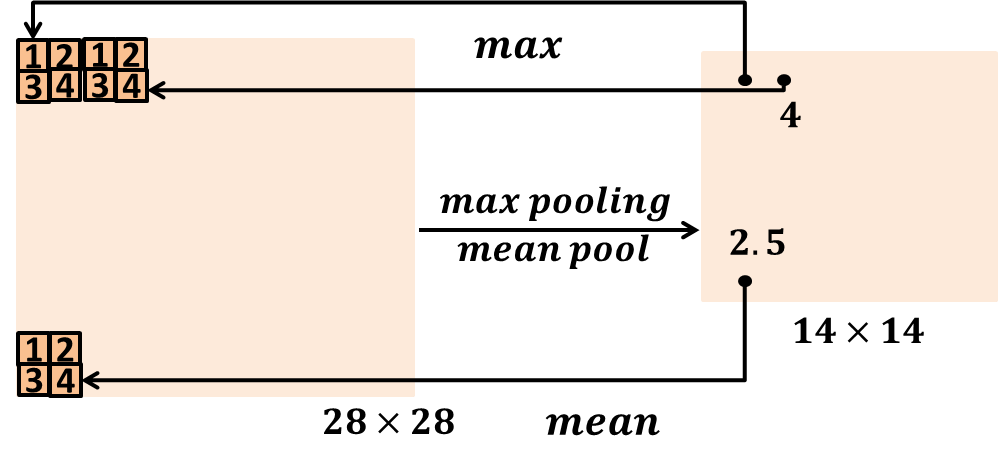
\includegraphics[height=4cm]{images/pooling_process.png}
            \caption{池化过程示意图}
            \label{fig:池化过程示意图}
            \end{figure}
            % \textcolor[rgb]{1 0 0}{todo:图片:池化过程示意图}\\
            把原图像($28\times 28$)中的相邻4个(上下左右)数值之间取最大值,作为输出。这样就从$28\times 28$变为$14\times 14$。当然,对于 mean pooling而言,我们取相邻的4个数值的平均作为输出。我们可以设置池化池/采样矩阵(采样矩阵的大小,例如:$4\times 4$)的大小为$m_p\times n_p$,但是,有必要让$m_y/m_p,n_y/n_p$为整数。
            \par
            考虑:1.为什么要采样;2.采样的误差传播如何进行;3.能否间隔采样。如何设计其它的采样方法,并且一定注意采样的误差传播应该易于进行。\\
            $3\clubsuit$:$C_3$为卷积层,输入6个$14\times 14$的矩阵,输出$16$个$12\times 12$的矩阵($12=14-3+1$),$S_2\to C_3$过程为卷积过程,但是,如果我们像$1\clubsuit$那样,对输入的6个矩阵的每一个矩阵都进行6次卷积操作,那么结果应该有$6$个或者$36$个输出矩阵。这$16$个输出矩阵式如何来的?我们应该清楚一点的是,输出矩阵的多少应该由卷积核的个数控制,比如:要形成16个输出矩阵,就设置16个卷积核,对于每个卷积核而言,无论有多少个输入图像与它进行卷积,都将其得到的结果相加,以形成1个输出。所以为了有16个输出就设置16个卷积核。现在的问题是:每个卷积核都应该和那几个输入图片(共6个)进行卷积呢?当然,可以进行全连接,即每个卷积核都要卷积6个输入。但是这样做会使计算量变得很大,为此,我们采用LeNet5的非全连接策略,其连接方式如表(\ref{tab:LeNet5的连接表})所示
            \begin{table}[htbp]
              \caption{LeNet5的连接表}
              \label{tab:LeNet5的连接表}
              \centering
              \begin{tabular}{c|llllllllllllllll}
              \toprule
              $S2\to C_3$&1  &2 &3  &4  &5  &6  &7  &8  &9  &10 &11 &12 &13 &14 &15 &16 \\
              \midrule
              1          &$@$ &  &   &   &$@$ &$@$ &$@$ &   &   &$@$ &$@$ &$@$ &$@$ &   &$@$ &$@$\\
              2          &$@$ &$@$&   &   &   &$@$ &$@$ &$@$ &   &   &$@$ &$@$ &$@$ &$@$ &   &$@$\\
              3          &$@$ &$@$&$@$ &   &   &   &$@$ &$@$ &$@$ &   &   &$@$ &   &$@$ &$@$ &$@$\\
              4          &   &$@$&$@$ &$@$ &   &   &$@$ &$@$ &$@$ &$@$ &   &   &$@$ &   &$@$ &$@$\\
              5          &   &  &$@$ &$@$ &$@$ &   &   &$@$ &$@$ &$@$ &$@$ &   &$@$ &$@$ &   &$@$\\
              6          &   &  &   &$@$ &$@$ &$@$ &   &   &$@$ &$@$ &$@$ &$@$ &   &$@$ &$@$ &$@$\\
              \bottomrule
              \end{tabular}
            \end{table}
            表(\ref{tab:LeNet5的连接表})中画$@$的表示对应的神经元(矩阵)连接,否则不连接。例如:$C_3$的第一个矩阵为
            \begin{align*}
            C_3^1 = f(S_2^1 w_1 + S_2^2 w_1 + S_2^3 w_1 + b)
            \end{align*}
            当然,这里还可以采取其他的非全连接方式。\\
            $4\clubsuit$:$S_4$为采样层(down sample)。如前,输入16个$12\times 12$矩阵,输出16个$6\times 6$矩阵。\\
            $5\clubsuit$:$F_5$为展开的特征层。该层的操作只是将$S_4$层得到的16个$6\times 6$矩阵展开合并为1个向量,以便输入到后面的神经网络等基本分类器当中。其实,$F_5$不仅可以在采样层$S_4$后对其展开,也可以在卷积层后对卷积层展开。\\
            $6/7\clubsuit$:是一个简单的分类器,比如BP和Softmax等。
            \par
            通过上面的分析,已经基本了解了CNN的网络结构与基本的操作(卷积和池化)。注:能否设置一个动态网络,随着训练的不断进行,网络结构也在发生变化?上面只是简单的描述了一下CNN的前向传播过程,下面,来建立数学模型,并求解网络参数(反向传播)。
        \subsubsection{CNN训练方式}
            \par
            先将CNN网络描述成神经元的形式,如图(\ref{fig:CNN网络的神经元形式})所示
            \begin{figure}[H]
            \centering
            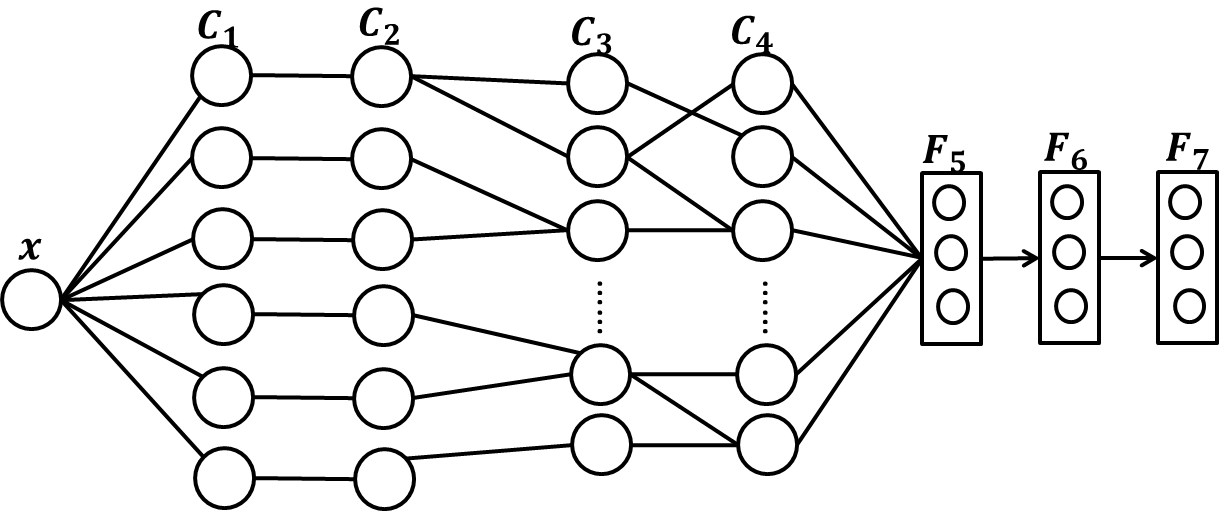
\includegraphics[height=3cm]{images/CNN_neural_form_of_the_network.jpg}
            \caption{CNN网络的神经元形式}
            \label{fig:CNN网络的神经元形式}
            \end{figure}
            % \textcolor[rgb]{1 0 0}{todo:图片:CNN网络的神经元形式}\\
            图(\ref{fig:CNN网络的神经元形式})中的每一个神经元表示一个矩阵(map)。更一般的,设样本集为$S = \{x^k,y^k\}_{k=1}^N $,共有$c$类,$y^k \in \{1,2,\dots,c\}$。设CNN网络共有$L$层(输入$x$不算一层),各层神经元个数为$n_l(l=1,2,\dots,L)$,记第$l$层神经元为$x^l$,$x^l = (x_1^l,x_2^l,\dots,x_{n_l}^l)$,$x_i^l$是矩阵(除了后面的BP分类器中的神经元外)。第$i$个神经元与第$j$个神经元连接的权重为$w_{ij}$(当然,许多神经元共用一个卷积核$w$),一般的,有几个输出图像就有几个卷积核。$b_j^l$为$l$层神经元$j$的偏置。
            \paragraph{CNN前向传播}(1)对卷积层而言,其输入输出可以表示为
            \begin{align*}
            x_j^l = f \left( \sum_{i=1}^{n_{l-1}}x_i^{l-1}\oplus w_{ij}^l + b_j^l \right)
            \end{align*}
            其中:$f$为普通可导函数,$\oplus$表示卷积等操作,并且是$l-1$层所有的神经元与$l$层的$j$神经元连接,且连接的各卷积核$w_{ij}$是不同的,这是一般的表述方式。我们记
            \begin{align*}
            u_j^l = \sum_{i=1}^{n_{l-1}}x_i^{l-1}\oplus w_{ij}^l + b_j^l
            \end{align*}
            为第$l$层第$j$神经元的输入,则$x_j^l$为其输出。
            \par
            (2)对池化层而言(采样层),其输入输出的表达式为
            \begin{align*}
            x_j^l = f \left( \beta_j^l \mathrm{down} \left( x_j^{l-1} \right)  + b_j^l \right)
            \end{align*}
            其中:$\mathrm{down}(x)$是对矩阵$x$进行下采样操作(均值池化、最大值池化),$\beta_j^l,b_j^l$为偏置。令
            \begin{align*}
            u_j^l = \beta_j^l \mathrm{down} \left( x_j^{l-1} \right)  + b_j^l
            \end{align*}
            为第$l$层第$j$个神经元的输入,$x_j^l$为其输出。
            \par
            (3)对小分类器而言
            \begin{align*}
            x^l = f(w^lx^{l-1}+b^l)\\
            \end{align*}
            或者写为
            \begin{align*}
            x_j^l = f \left( w_{\cdot j}^l x^{l-1} + b_j^l \right) = f \left(  \sum_{i=1}^{n_{l-1}}x^{l-1}+b_j^l \right)
            \end{align*}
            我们仍然令
            \begin{align*}
            u^l = w^lx^{l-1}+b^l
            \end{align*}
            为第$l$层的输入,$x^l$为输出。
            \paragraph{CNN反向传播}先来表示网络输出值$t$和样本真实值的误差,以便构建“离差平方和目标”。
            对于$N$个样本$S=\{x^k,y^k\}_{k=1}^N$,$c$个类别,其误差平方可以表示为
            \begin{align*}
            E = \frac{1}{2}\sum_{n=1}^N\sum_{k=1}^c (t_k^n-y_k^n)^2
            \end{align*}
            其中:$t^n$表示第$n$个样本的网络输出值/估计值。记$e^n\in R^c/\{0,1\}^c$为第$n$个样本的误差,$E^n$为第$n$个样本的误差平方,有
            \begin{align*}
            & E = \sum_{n=1}^N E^n\\
            & E^n = \frac{1}{2}\sum_{k=1}^c (t_k^n - y_k^n)^2 = \frac{1}{2}||t^n - y^n||^2
            \end{align*}
            令$\theta \overset{\Delta}{=} (w,b)$。$E$关于$\theta$求导,有
            \begin{align*}
            \frac{\partial E}{\partial \theta} = \sum_{n=1}^N \frac{\partial E^n}{\partial \theta}
            \end{align*}
            下面,来求解$ \frac{\partial E^n}{\partial \theta}$。
            \par
            (1)对小分类器而言,和前面介绍的BP是一样的,这里我们再写一次。
            \begin{align*}
            E^2 = \frac{1}{2}||f(u^L) - t^n||^2 = \frac{1}{2}||f(w^Lx^{l-1}+b^L) - t^n||^2 = \frac{1}{2} ||y^n - t^n||^2
            \end{align*}
            对所有的$l$(小分类器的层),$E^n$关于$b$求导有
            \begin{align*}
            \frac{\partial E^n}{\partial b^L} = \frac{\partial E^n}{\partial u^L} \frac{\partial u^L}{\partial b^L}
            \end{align*}
            而$\frac{\partial u^L}{\partial b^L} = 1$,所以我们要求$\frac{\partial E^n}{\partial u^l}$。定义$\delta^L = \frac{\partial E^n}{\partial u^l}$,有
            \begin{align*}
            & \delta^L = \frac{\partial E^n}{\partial u^L} = \frac{\partial }{\partial u^L}\frac{1}{2}||f(u^L) - t^n||^2 = (f(u^L )-t^n) f'(u^L) = e^n f'(u^L)\\
            & \delta ^l = \frac{\partial E^n}{\partial u^l} (w^{l+1})^\mathrm{T}\delta^{l+1}f'(u^l)\quad l=L-1,L-2,\dots,
            \end{align*}
            同理,$E^n$关于$w$求导,有
            \begin{align*}
            \frac{\partial E^n}{\partial w^l} = \frac{\partial E^n}{\partial u^l}\frac{\partial u^l}{\partial w^l} = x^{l-1}(\delta^l)^\mathrm{T}
            \end{align*}
            \par
            (2)对卷积层而言。卷积层的反向传播示意图如图(\ref{fig:卷积层的反向传播示意图})所示
            \begin{figure}[H]
            \centering
            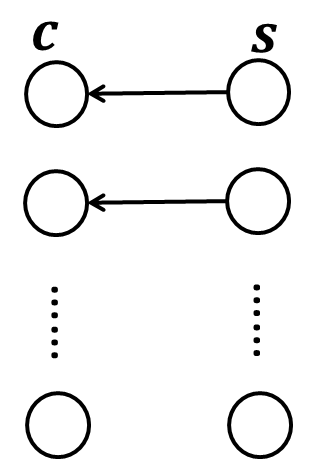
\includegraphics[height=4cm]{images/The_reverse_propagation_of_the_convolution_layer.jpg}
            \caption{卷积层的反向传播示意图}
            \label{fig:卷积层的反向传播示意图}
            \end{figure}
            % \textcolor[rgb]{1 0 0}{todo:图片:卷积层的反向传播示意图}
            \begin{align*}
            \delta_j^l = \beta_j^{l+1} \left( f'(u_j^l)\cdot \mathrm{up}(\delta_j^{l+1}) \right)
            \end{align*}
            其中:$\mathrm{up}(\cdot)$是上采样操作,与$\mathrm{down}(\cdot)$相反。如果下采样的池化池/采样矩阵的大小为$n\times n$,则$\mathrm{up}(x)$写为
            \begin{align*}
            \mathrm{up}(x) = x \otimes I_{n\times n}
            \end{align*}
            这里的$\otimes $表示Kronecker乘积。比如,在$S$层中第一个神经元的误差矩阵为
            \begin{align*}
            e=
            \begin{pmatrix}
            1 & 2\\
            3 & 4
            \end{pmatrix}
            \end{align*}
            而$S$的第一个神经元是$C$的第一个神经元经过最大下采样缩小2倍($n=2$)得到的,那么
            \begin{align*}
            \mathrm{up}(e) =
            \begin{pmatrix}
            1 & 1 & 2 & 2\\
            1 & 1 & 2 & 2\\
            3 & 3 & 4 & 4\\
            3 & 3 & 4 & 4\\
            \end{pmatrix}
            \end{align*}
            \par
            现在,得到了$l$层神经元$j$的误差$\delta_j^l$,接下来,要把误差下分到权重$w_j^l$和$b_j^l$上
            \begin{align*}
            & \frac{\partial E^n}{\partial b_j} = \sum_{u,v} \left( \delta_j^l \right)_{uv} \\
            & \frac{\partial E^n}{\partial w_{ij}^l} = \sum_{u,v} \left( \delta_j^l \right)_{uv} \left( p_i^{l-1} \right)_{uv}
            \end{align*}
            其中:$ \sum_{u,v} \left( \delta_j^l \right)_{uv}$表示将$\delta_j^l$逐元素相加,$(p_i^{l-1})_{uv}$是$x_i^{l-1}$在卷积时候,与$w_{ij}^l$逐元素相乘的pitch,输出卷积层某个图像的$uv$位置是由上一层$uv$位置的pitch与卷积核$w_{ij}^l$逐元素相乘的结果。在MATLAB中可以通过下面的命令实现
            \begin{align*}
            \frac{\partial E^n}{\partial w_{ij}^l} = \mathrm{rot}180 (\mathrm{conv2}(x_i^{l-1},\mathrm{rot180}(\delta_j^l),'valid'))
            \end{align*}
            示例:卷积层的误差传递如图(\ref{fig:卷积层误差传递示意图})所示
            \begin{figure}[H]
            \centering
            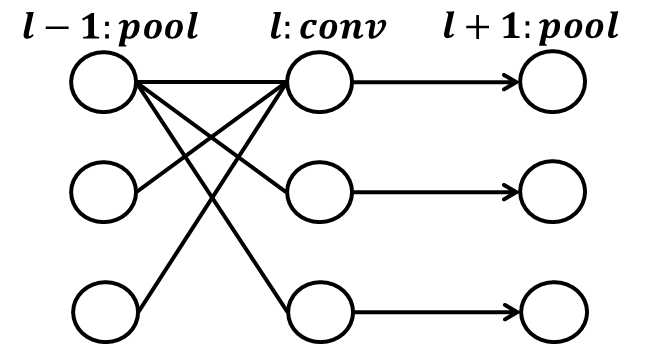
\includegraphics[height=3cm]{images/Convolution_layer_error_transfer_diagram.jpg}
            \caption{卷积层误差传递示意图}
            \label{fig:卷积层误差传递示意图}
            \end{figure}
            % \textcolor[rgb]{1 0 0}{todo:图片:卷积层误差传递示意图}\\
            假设$l+1$层的pool层大小为$2\times 2$,并且此时pool后的$\delta_j^{l+1}$是
            \begin{math}
            \left(
            \begin{smallmatrix}
            1 & 3\\
            2 & 4
            \end{smallmatrix}
            \right)
            \end{math}
            \ding{172}如果将$l$层(卷积层)mean pool到$l+1$层,则$l$层$\delta_j^l$应为$4\times 4$,为
            \begin{align*}
            \mathrm{up}(\delta_j^{l+1}) =
            \begin{pmatrix}
            1 & 1 & 3 & 3\\
            1 & 1 & 3 & 3\\
            2 & 2 & 4 & 4\\
            2 & 2 & 4 & 4\\
            \end{pmatrix}
            \end{align*}
            又因为是均值采样且反向传播时,误差总和不变,所以卷积层$l$要对每个值平摊,于是误差变为
            \begin{align*}
            \begin{pmatrix}
            0.25 & 0.25 & 0.75 & 0.75\\
            0.25 & 0.25 & 0.75 & 0.75\\
            0.5  & 0.5  & 1    & 1   \\
            0.5  & 0.5  & 1    & 1   \\
            \end{pmatrix}
            \end{align*}
            $\mathrm{up}(x)$可以通过MATLAB中的kron函数实现。\ding{173}如果是将$l$层max pool到$l+1$层,则需要在前向传播中记录pool区域中的最大值的位置,以便把误差分给相应位置。假如我们在
            \begin{math}
            \left(
            \begin{smallmatrix}
             & & &*\\
             &*& & \\
            *& & & \\
             & &*& \\
            \end{smallmatrix}
            \right)
            \end{math}
            位置取得最大值,则
            \begin{align*}
            \delta_j^l =
            \begin{pmatrix}
            0 & 0 & 0 & 3\\
            0 & 1 & 0 & 0\\
            2 & 0 & 0 & 0\\
            0 & 0 & 4 & 0\\
            \end{pmatrix}
            \end{align*}
            \par
            上面给出了$\delta_j^l$的求法,现在给出$\frac{\partial E^n}{\partial b_j^l},\frac{\partial E^n}{\partial w_{ij}^l}$的求法。这里不考虑非线性函数$f$和$\beta_j^l$,因此,pool层前面是没有权值的,也就没有所谓的权值的导数了。假设现在要求
            \begin{align*}
            & \frac{\partial E^n}{\partial b_j} = \sum_{u,v} \left( \delta_j^l \right)_{uv} \\
            & \frac{\partial E^n}{\partial w_{ij}^l} = x_i^{l-1}\odot \delta_j^l
            \end{align*}
            其中:$\odot$表示矩阵相关操作(反卷积),可以用conv2函数实现,但是要将$\delta_j^l$旋转$180^\circ$,即
            \begin{align*}
            \mathrm{conv2}(x_i^{l-1},\mathrm{rot180}(\delta_j^l),'valid')
            \end{align*}
            设第$l-1$层的第$i$个图像(矩阵)$x_i^{l-1}$大小为$4\times 4$的
            \begin{math}
            \left(
            \begin{smallmatrix}
            16 & 2  & 3  & 13\\
            5  & 11 & 10 & 8 \\
            9  & 7  & 6  & 12\\
            4  & 14 & 15 & 1 \\
            \end{smallmatrix}
            \right)
            \end{math}
            ,第$l$层的第$j$个神经元的误差$\delta_j^l$为$3\times 3$的
            \begin{math}
            \left(
            \begin{smallmatrix}
            0.8  & 0.1 &  0.6\\
            0.3  & 0.5 &  0.7\\
            -0.4 & 0   & -0.2\\
            \end{smallmatrix}
            \right)
            \end{math}
            ,这时的$w_{ij}^l$的导数矩阵的大小为$2\times 2$且其结果为
            \begin{align*}
            \begin{pmatrix}
            16 & 2  & 3  & 13\\
            5  & 11 & 10 & 8 \\
            9  & 7  & 6  & 12\\
            4  & 14 & 15 & 1 \\
            \end{pmatrix}
            \odot
            \begin{pmatrix}
            0.8  & 0.1 &  0.6\\
            0.3  & 0.5 &  0.7\\
            -0.4 & 0   & -0.2\\
            \end{pmatrix}
            =
            \begin{pmatrix}
            20.4 & 2.8\\
            4.9 & 12.7\\
            \end{pmatrix}
            \end{align*}
            此时偏置$b_j^l$的导数为1.2,即将$\delta_j^l$的元素相加即可$0.8+0.1-0.6+0.3+0.5+0.7-0.4-0.2=1.2$。
            \par
            (3)对池化层而言。这里最困难的是计算$\delta_j^l$,一旦得到了它,我们只要更新偏置参数$\beta,b$就可以了。如果池化层$l$与下一层卷积层$l+1$是全连接,那么就可以通过BP来计算采样层$\delta_j^l$了。要计算卷积核的梯度,所以必须要找到输入矩阵中哪部分(patch)对应输出矩阵的哪一个像素。这里,要找到当前层(pool)的$\delta_j^l$矩阵的哪一patch对应下一层(卷积层)的$\delta^{l+1}$的给定像素,然后用反向传播传递回来
            \begin{align*}
            \delta_j^l = f'(u_j^l)\cdot \mathrm{conv2} \left( \delta_j^{l+1},\mathrm{rot180}(k_j^{l+1}),'full' \right)
            \end{align*}
            \par
            下面,就可以把误差/灵敏度$\delta_j^l$传递给$\beta,b$了
            \begin{align*}
            \frac{E^n}{\partial b_j^l} =  \sum_{u,v}(\delta_j^l)w
            \end{align*}
            而对于乘性偏置$\beta$,因为涉及到了前向传播中下采样的计算,所以,最好在前向传播中保存好这些矩阵,这样,在反向传播中就不用重新计算了。令
            \begin{align*}
            d_j^l = \mathrm{down}(x_j^{l-1})
            \end{align*}
            则
            \begin{align*}
            \frac{\partial E^n}{\partial \beta_j} = \sum_{u,v} \left( \delta_j^l d_j^l \right) _{uv}
            \end{align*}
            示例:池化层的反向传播示意图如图(\ref{fig:池化层的反向传播示意图})所示
            \begin{figure}[H]
            \centering
            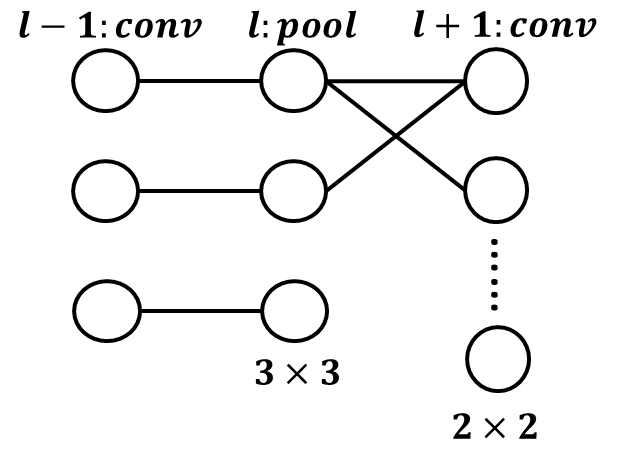
\includegraphics[height=3cm]{images/The_reverse_propagation_of_the_pool_layer.jpg}
            \caption{池化层的反向传播示意图}
            \label{fig:池化层的反向传播示意图}
            \end{figure}
            % \textcolor[rgb]{1 0 0}{todo:图片:池化层的反向传播示意图}\\
            假设$l$层的某个矩阵$x_j^l$的大小为$3\times 3$,第$l+1$层有2个卷积核$w_1^l,w_2^l$,卷积核的大小为$2\times 2$,则在前向传播时,第$l+1$层会有2个$2\times 2$的输出矩阵$x^{l+1}$。设2个卷积核为
            \begin{math}
            \left(
            \begin{smallmatrix}
            0.1 & 0.2 \\
            0.2 & 0.4\\
            \end{smallmatrix}
            \right)
            \end{math}
            和
            \begin{math}
            \left(
            \begin{smallmatrix}
            -0.3 & 0.1 \\
            0.1 & 0.2\\
            \end{smallmatrix}
            \right)
            \end{math}
            。反向传播时,假设已经知道第$l+1$层2个输出图的误差$\delta_1^{l+1}$和$\delta_2^{l+2}$为
            \begin{math}
            \left(
            \begin{smallmatrix}
            1& 3 \\
            2& 2\\
            \end{smallmatrix}
            \right)
            \end{math}
            和
            \begin{math}
            \left(
            \begin{smallmatrix}
            2& 1 \\
            1& 1\\
            \end{smallmatrix}
            \right)
            \end{math}
            。注:1.矩阵大小为多大,误差$\delta$就为多大,每个矩阵元素都有误差/灵敏度;2.假设pool到conv是全连接。
            \par
            那么,我们就将$w_j^{l+1}$和$\delta_j^{l+1}$实现conv2操作
            \begin{align*}
            \mathrm{conv2}(\delta_j^{l+1},\mathrm{rot180}(w_j^{l+1}),'full')
            \end{align*}
            其中,conv2将$\delta_j^{l+1}$填充'full'为
            \begin{math}
            \left(
            \begin{smallmatrix}
            0 & 0 & 0 & 0\\
            0 & 1 & 3 & 0\\
            0 & 2 & 2 & 0\\
            0 & 0 & 0 & 0\\
            \end{smallmatrix}
            \right)
            \end{math}
            和
            \begin{math}
            \left(
            \begin{smallmatrix}
            0 & 0 & 0 & 0\\
            0 & 2 & 1 & 0\\
            0 & 1 & 1 & 0\\
            0 & 0 & 0 & 0\\
            \end{smallmatrix}
            \right)
            \end{math}
            然后再和旋转$180^\circ$的$w_j^{l+1}$进行卷积操作,有
            \begin{align*}
            &
            \begin{pmatrix}
            0 & 0 & 0 & 0\\
            0 & 1 & 3 & 0\\
            0 & 2 & 2 & 0\\
            0 & 0 & 0 & 0\\
            \end{pmatrix}
            \odot
            \begin{pmatrix}
            0.1 & 0.2 \\
            0.2 & 0.4 \\
            \end{pmatrix}
            =
            \begin{pmatrix}
            0.1 & 0.5 & 0.6\\
            0.4 & 1.6 & 1.6\\
            0.4 & 1.2 & 0.8\\
            \end{pmatrix}\\
            &
            \begin{pmatrix}
            0 & 0 & 0 & 0\\
            0 & 2 & 1 & 0\\
            0 & 1 & 1 & 0\\
            0 & 0 & 0 & 0\\
            \end{pmatrix}
            \odot
            \begin{pmatrix}
            -0.3 & 0.1 \\
            0.1 & 0.2 \\
            \end{pmatrix}
            =
            \begin{pmatrix}
            -0.6 & -0.1 & 0.1\\
            -0.1 & 0.3 & 0.3\\
            0.1 & 0.3 & 0.2\\
            \end{pmatrix}
            \end{align*}
            则$l$层$j$矩阵的灵敏度$\delta_j^l$为$3\times 3$,是上述2个矩阵的和
            \begin{align*}
            \delta_j^l =
            \begin{pmatrix}
            0.1 & 0.5 & 0.6\\
            0.4 & 1.6 & 1.6\\
            0.4 & 1.2 & 0.8\\
            \end{pmatrix}
            +
            \begin{pmatrix}
            -0.6 & -0.1 & 0.1\\
            -0.1 & 0.3 & 0.3\\
            0.1 & 0.3 & 0.2\\
            \end{pmatrix}
            =
             \begin{pmatrix}
            -0.5 & 0.4 & 0.9\\
            0.3 & 1.9 & 1.9\\
            0.5 & 1.5 & 1\\
            \end{pmatrix}
            \end{align*}
            \par
            (4)学习特征矩阵的组合。大部分时候,通过卷积多个输入矩阵(maps),然后再对这些卷积值求和得到一个输出map,这样做的效果往往较好。在一些文献中,如LeNet中,一般是选择哪些输入maps组合在一起进行输入。现在,我们让CNN在训练过程中自己学习这些组合,即让网络自己挑选哪些输入maps进行组合。我们用$\alpha_{ij}$表示第$j$个输出的map中的$i$个输入map的权重或贡献。这样,第$j$个输出map就可以表示为
            \begin{align*}
            x_j^l =f \left( \sum_{i=1}^{n_l-1} \alpha_{ij}(x_i^{l-1}\oplus w_i^l) + b_j^l \right)
            \end{align*}
            要求$\alpha_{ij}$要满足
            \begin{align*}
            &\sum_i \alpha_{ij} = 1\\
            &0 \leqslant \alpha_{ij} \leqslant 1
            \end{align*}
            上述约束可以通过将变量$\alpha_{ij}$表示为一组无约束的隐含权值$c_{ij}$的softmax函数来加强(因为softmax的因变量是自变量的指数函数,它们的变化率会不同)
            \begin{align*}
            \alpha_{ij} = \frac{e^{c_{ij}}}{\sum_ke^{c_{kj}}}
            \end{align*}
            \par
            因为对于一个固定的$j$而言,每组权值$c_{ij}$都是和其它组的权值独立的,所以为了方便描述,我们把下标$j$去掉,只考虑一个map的更新,其他map的更新情况是一样的,只是索引$j$不同而已。softmax函数的导数表示为
            \begin{align*}
            \frac{\partial \alpha_k}{\partial c_i} = \delta_{ki}\alpha_i - \alpha_i\alpha_k
            \end{align*}
            这里的$\delta$是Kronecker delta。误差$E^n$对第$l$层变量$\alpha_i$的导数为
            \begin{align*}
            \frac{\partial E^n }{\partial \alpha_i} = \frac{\partial E^n}{\partial u^l} \frac{\partial u^l}{\partial \alpha_i} = \sum_{uv} \left( \delta ^l\odot(x_i^{l-1}\oplus w_i^l)  \right)
            \end{align*}
            其中:$\odot$表示元素操作,$\oplus$表示卷积操作。最后,$E^n$对$c_i$求导,有
            \begin{align*}
            \frac{\partial E^n}{\partial c_i} &= \sum_k \frac{\partial E^n}{\partial \alpha_k}\frac{\partial \alpha_k}{\partial c_i}\\
            &=\alpha_i \left( \frac{\partial E^n}{\partial \alpha_i} - \sum_{k}\frac{\partial E^n}{\partial \alpha_k}\alpha_k \right)
            \end{align*}
            \par
            (5)强加稀疏性组合。为了限制$\alpha_i$是稀疏的,也就是限制一个输出map与某些而非全部输入maps链接,我们在整体代价函数中增加稀疏约束项$\Omega(\alpha)$。对单一样本而言,重写代价函数为
            \begin{align*}
            \tilde{E}^n = E^n + \lambda \sum_{i,j} |(\alpha)_{ij}| = E^n + \Omega(\alpha)
            \end{align*}
            我们仍将$\tilde{E}^n$关于参数求导,这里主要是$\Omega(\alpha)$对权值$c_i$求导。先求$\Omega(\alpha)$关于$\alpha_i$的导数,再求对$c_i$的导数,有
            \begin{align*}
            & \frac{\partial \Omega}{\partial \alpha_i} = \alpha \mathrm{sign}(\alpha_i)\\
            \end{align*}
            所以权重$c_i$的梯度为
            \begin{align*}
            \frac{\partial \tilde{E}}{\partial c_i} = \frac{\partial E}{\partial c_i} + \frac{\partial \Omega }{\partial c_i}
            \end{align*}
        \subsubsection{CNN的问题}
            \par
            % \textcolor[rgb]{1 0 0}{(1)自带
            % (2)DeepLearnToolbox
            % }
            \begin{enumerate}
            \item 梯度消失。无论是ANN(MLP)、CNN还是后面要介绍的RNN,如果网络层数过多,就会出现梯度消失/爆炸现象。比如:$\frac{\partial E}{\partial w^l}$,当$L$很大而$l =1$时,$\frac{\partial E}{\partial w^1} = (10^{-10})_{n\times n}$。这时权重$w$的更新非常小,几乎不动。解决方法:1.减少层数$L$;2.增大学习率$\eta$;3.使用ReLu作为传递函数。
            \item 随机梯度下降的参数选取。如何选取批量样本大小以及学习率$\eta$。
            \item 参数$\theta \overset{\Delta }{=}(w,b)$的初始化。
            \item 样本归一化。
            \end{enumerate}

    \subsection{AlexNet}
        \par
        2012年,Hinton教授及其2个学生Alex kvizhevsky和Ilya Sutskever提出一种改进的深层CNN网络 - AlexNet,并将其运用到Image Net的ILSVRC2012中,取得了当时最好的成绩:在top-1和top-5上的误差率为$37.5\%$和$17.0\%$。
        \par
        ImageNet(http://www.image-net.org)是李菲菲组的图像库。ImageNet设想为全世界的教育工作者、研究工作者提供图片资源。ImageNet不拥有图片的版权,只提供图片的缩略图和url。从某种程度上讲,它可以视为图像搜索引擎。ILSVRC使用ImageNet的一个子集,共1000个类别,每个类别大约包含1000张图片,训练集为12万张,验证集为5万张,测试集为1万张。输入图像的大小为$256\times 256 \times 3$。在AlexNet网络中,随机提取$224\times 224$个像素点,然后crop\footnote{注:crop为将图片进行4个边界crop和中心crop。}。crop后实际输入到AlexNet网络的图像大小为$227\times 227\times 3$(RGB图像)。
        \par
        AlexNet是一种经典的DeepCNN,它由5层convolution layer、2层fully connected layer和1个label layer(1000类)组成,是一个8层的CNN网络,但是这里的Convolution layer和CNN中的不同,它是许多网络层的组合,比如:convolution layer1是由1个卷积层、1个maxpool和1个LRN共同构成。AlexNet的网络结构如图(\ref{fig:AlexNet网络结构图1})所示
            \begin{figure}[H]
            \centering
            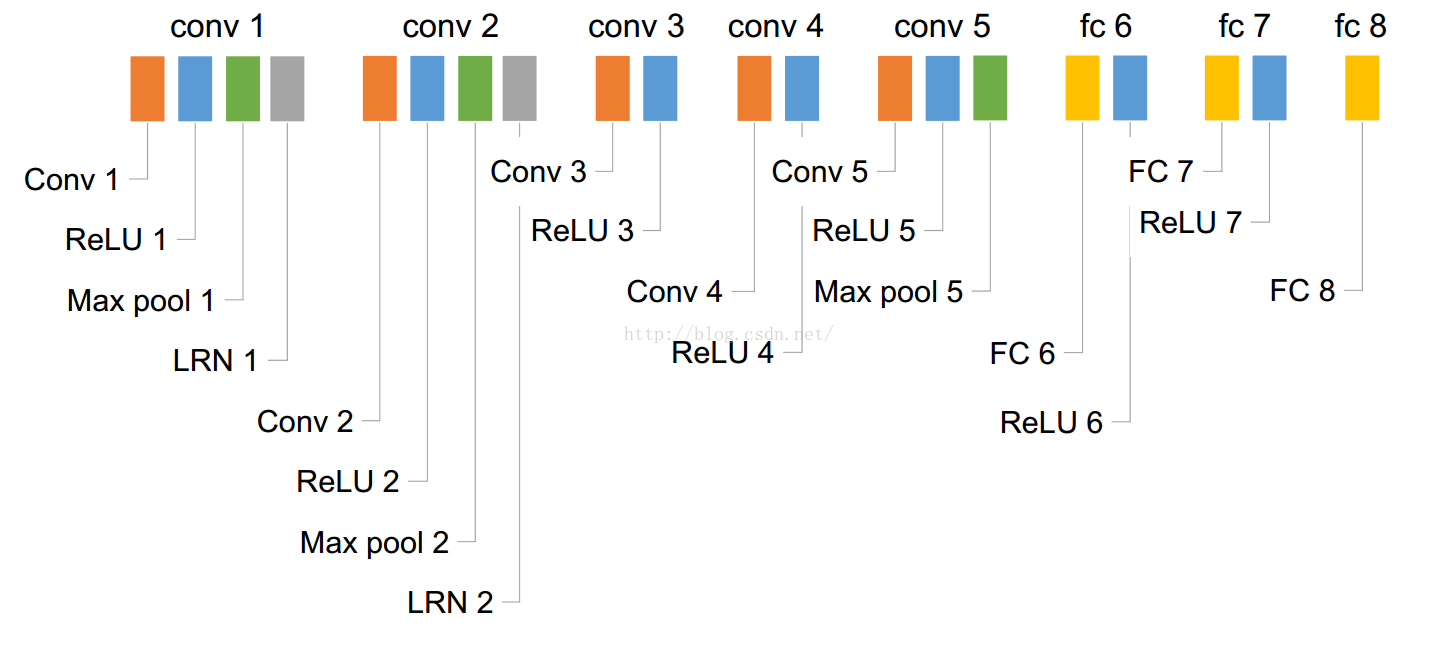
\includegraphics[width=8cm]{images/AlexNet1.jpg}
            \caption{AlexNet网络结构图1}
            \label{fig:AlexNet网络结构图1}
            \end{figure}
        % \textcolor[rgb]{1 0 0}{todo:图片:AlexNet网络结构图1}
        \par
        从上面的网络示意图(\ref{fig:AlexNet网络结构图1})中,我们可以看到,与传统的CNN相比,AlexNet除了网络层数更深之外,还多了Relu和LRN层。这个大的网络包含了6千万个参数和65万个神经元,并利用了Rleu、dropout、data augmentation等技术来防止过拟合。下面,我们来介绍AlexNet中的这些技术。
        \par
        (1)Relu。在前面的神经网络章节中,介绍传递函数时,我们已经介绍了Relu传递函数。我们用Relu来代替传统的sigmoid函数,其好处有3,\ding{172}在采用sigmoid传递时,计算需要指数运算,此运算相对而言计算量大,并且,在反向传播求梯度时,求导涉及到除法,除法的计算量仍然大;\ding{173}在sigmoid传递时,当网络深度很大时,容易出现梯度消失现象,因为在sigmoid接近饱和区域时,变化太缓慢,梯度趋于0,造成信息损失;\ding{174}Relu使一部分神经元的输出为0,使网络具有稀疏性,并减少了参数的相互依赖关系。
        \par
        (2)Local Response Normalization, LRN(局部归一化)。Relu传递函数本身其实是不对输入做归一化的,从而避免出现饱和现象。如果训练样本经过卷积网络产生正响应输入到Relu的,则就可以对该神经元的参数进行相应的学习,不过AlexNet发现,在Relu后面加上一个局部归一化部分,则会使网络达到更好的泛化效果
        \begin{align*}
        b_{xy}^i = a_{xy}^i\Bigg/ \left( k+\alpha\sum_{j=\max(0,i-n/2)}^{\min (N-1,i+n/2)} (a_{xy}^i)^2\right)^\beta
        \end{align*}
        其中:$a_{xy}^i$表示输入maps的$(x,y)$位置做第$i$次卷积并通过Relu单元的结果,而$b_{xy}^i$是相应归一化的结果,$n$是指相同位置的第$i$次前后附近的卷积核的数目,而$N$是总的卷积次数。选取邻近的$n$个特征图(maps),在maps的空间位置$(x,y)$一次平方,然后求和,乘以$\alpha$,加上$k$。Alex在原文中是$k=1$,$n=5$,$\alpha=10^{-4}$,$\beta = 0.75$,并且与不做局部归一化进行比较,在top-1和top-5上分别提到了$1.4\%$和$1.2\%$,并且在CIFAR10中的结果也有提高。
        \par
        (3)重叠pooling层。普通的采样层(如前面CNN的池化层那样),采样窗口大小为$2\times 2$。我们可以以步长$s$进行划分,如果是普通采样,$s=z(=2)$,即采样窗口不重叠,我们利用$z\times z$大小的采样窗口,隔$s$步($s$个像素点)蹦一下,进行采样。而重叠pool就像它的名字一样,前后2个采样窗口$(z\times z)$是有重叠的,即$s<z$。无重叠pool如图(\ref{fig:有无重叠的pool示意图})(a)所示,有重叠pool如图(\ref{fig:有无重叠的pool示意图})(b)所示
            \begin{figure}[H]
              \centering
              \begin{varwidth}[t]{\textwidth}
                \vspace{0pt}
                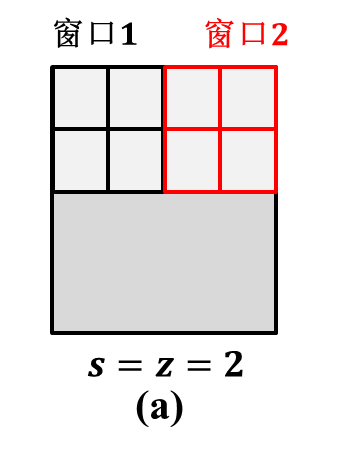
\includegraphics[height=4cm]{images/yes_or_no_overlapping_pool1.jpg}
              \end{varwidth}
              \qquad\qquad
              \begin{varwidth}[t]{\textwidth}
                \vspace{0pt}
                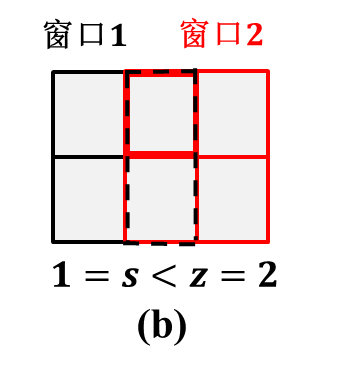
\includegraphics[height=4cm]{images/yes_or_no_overlapping_pool2.jpg}
              \end{varwidth}
                \caption{有无重叠的pool示意图}
                \label{fig:有无重叠的pool示意图}
            \end{figure}
        % \textcolor[rgb]{1 0 0}{todo:图片:有无重叠的pool示意图}\\
        当然,如果采用有重叠的pool方式\footnote{注:有学者认为,在训练一个良好的生成模型时,弃用pool层也是很重要的,如VAE和GAN。},可能使采样结果重复(对maxpool而言)。另外,实验表明,maxpool优于meanpool。Alex实验表明,使用$s=2,z=3$的有重叠pool比使用$s=z=2$的无重叠pool效果要好,在top-1和top-5上提高$0.4\%$和$0.3\%$。
        \par
        (4)过拟合。AlexNet网络有6千万个参数,而训练样本的类别只有1000类,这不足以让我们来学习这么大的网络,因此我们要考虑网络的过拟合。文中提到了2个防止过拟合的策略,一个是Data Augmantation(这个我们不介绍),一个是dropout。组合预测是一种非常成功的减小预测误差的手段,但它训练要花费好几天的时间,对大型网络而言,更是困难。然而,最近推出的dropout技术是一种非常有效的模型组合方法,它的训练只花费2倍的单模型的时间。dropout是Hinton在Improving neural networks by preventing co-adaption中提出的,以0.5概率随机将隐含层中的各神经元输出置为0。以这种方式丢弃的神经元既不参与前向传播,也不参与反向传播,所以对每个输入样本而言,该神经网络都是一个随机得到不确定的网络。但是,所有这些结构之间共享权重,即权重的更新照旧。这样得到的参数能够适应不同情况下的网络结构,提高了系统的鲁棒性。AlexNet的前2个full connected(FC)层使用了dropout方法,所以在测试时,应该注意,对每个被dropout的神经元的输出乘上一个0.5,以合理的逼近预测输出分布的几何均值。
        \par
        (5)学习过程。下面介绍的内容在本书的其它部分皆有详细的介绍。AlexNet网络的目标函数可以设置为1.log-loss;2.softmax log-loss;3.p-distance loss。对于AlexNet训练参数的设置,AlexNet训练时使用批量梯度下降算法SGD,批量大小(batch size)为128。参数更新使用动量(momentum)更新方法,weight deccy设置为0.0005,更新公式为
        \begin{align*}
        & v_{i+1} = 0.9v_i-0.0005\cdot\epsilon\cdot w_i - \epsilon\cdot\Big<\frac{\partial L}{\partial w}\Big |_{w_i}\Big>_{D_i}\\
        & w_{i+1} = w_i+v_{i+1}
        \end{align*}
        其中:$i$为第$i$个批量样本(每个批量更新一次参数),$v$为动量,$\epsilon$为学习率,$\Big<\frac{\partial L}{\partial w}\Big |_{w_i}\Big>_{D_i}$是第$i$个批量$D_i$的目标$L$关于$w$的方向导数在$w_i$的值。
        \par
        网络的初始权重为$w_0\sim N(0,0.01)$,而2、4、5卷积层的偏置b及全连接层FC的偏置初始化都为1,剩下的偏置初始化为0。对于学习率$\epsilon$,每次对当前的学习率除以10,直到交叉验证CV的error rale不再更新为止。Alex的学习率初始值为0.01,验证3次就终止。AlexNet在ImageNet的1.2百万张图片上,大概90次停止,在NVIDIA GTX 580 GPU上跑了5到6天。
        \par
        (6)网络框架。进入CNN,我们也基本上正式进入了深度学习搭建、调参之旅,说实话,旅途坑很多。这里插入2张图片(\ref{fig:AlexNet网络框架图}),上图是AlexNet的网络数字流程图,下图是AlexNet的双GPU图。
        \begin{figure}[H]
          \centering
          \begin{varwidth}[t]{\textwidth}
            \vspace{0pt}
            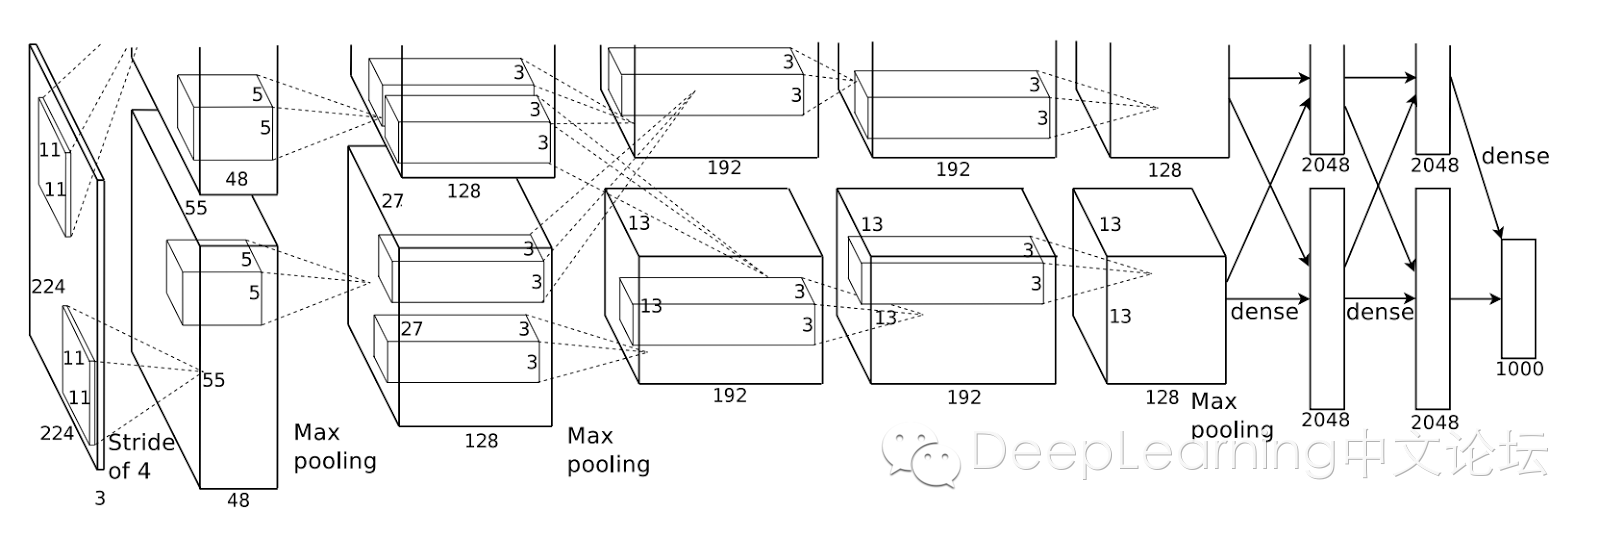
\includegraphics[height=4cm]{images/AlexNet_net_digital_flow_chart.jpg}
          \end{varwidth}
          \qquad
          \begin{varwidth}[t]{\textwidth}
            \vspace{0pt}
            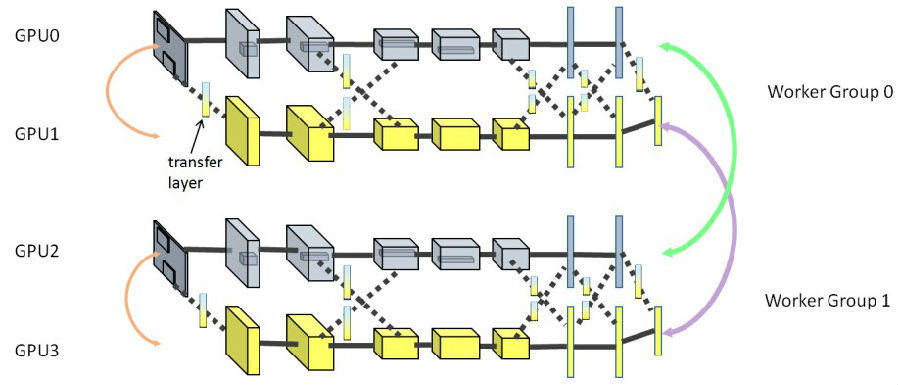
\includegraphics[height=4cm]{images/AlexNet_double_GPU.jpg}
          \end{varwidth}
          \caption{AlexNet网络框架图}
          \label{fig:AlexNet网络框架图}
        \end{figure}
        % \textcolor[rgb]{1 0 0}{todo:图片:AlexNet的网络数字流程图}\\
        % \textcolor[rgb]{1 0 0}{todo:图片:AlexNet的双GPU图}\\

    \subsection{NiN}
        \par
        2014年Min Lin的Network in Network(NiN)\cite{2014.MinLin}是当时少有的对CNN卷积层进行改进的文章。文章就CNN框架提出了2种改进方案:1、mloconv替代conv;2、平均池(average pooling)替代CNN的全连接。
        \subsubsection{mloconv替代conv}
            \par
            NiN使用mlpconv来替代原来的conv层,mlpconv实际上是在conv层上加上mlp。因为conv是线性的,而mlp是非线性的,后者能够得到更高的抽象层,泛化能力更强。在跨通道的情况下(cross channel,cross feature map),mlpconv等价于卷积层加上$1\times 1$卷积层,所以mlpconv也称为cccp层。借助这个机会,我们再来看一下conv。其实CNN和MLP有很深的渊源,我们可以将CNN展成向量来观察二者之间的相似性,这里我们就不做了。
            \par
            (1)conv。传统的conv是给定一张图片(map)$x$,我们用一个卷积核$w$扫描这张图片,以实现卷积,如图(\ref{fig:传统的conv})所示
            \begin{figure}[H]
            \centering
            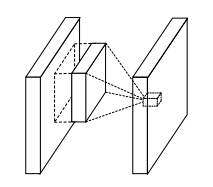
\includegraphics[height=3cm]{images/traditional_conv.jpg}
            \caption{传统的conv}
            \label{fig:传统的conv}
            \end{figure}
            % \textcolor[rgb]{1 0 0}{todo:图片:传统的conv}\\
            这其实是权重共享技术,因为原输入$x$共享了一个卷积核/权重$w$。比如,我们将$x$展开成向量,将卷积核$w$展开成向量,如图(\ref{fig:卷积核展开示意图})所示
            \begin{figure}[H]
            \centering
            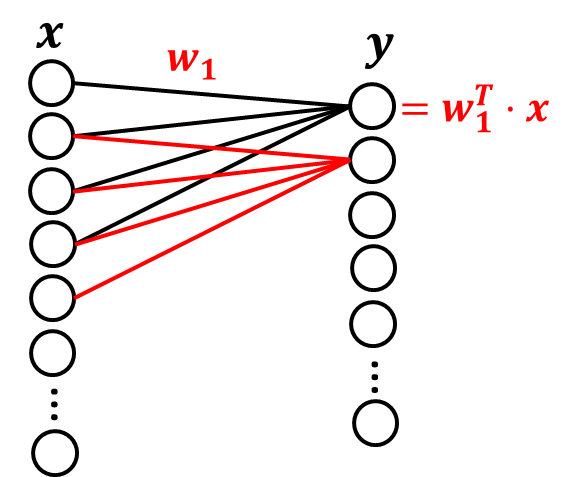
\includegraphics[height=3cm]{images/Convolution_core_unfold.jpg}
            \caption{卷积核展开示意图}
            \label{fig:卷积核展开示意图}
            \end{figure}
            % \textcolor[rgb]{1 0 0}{todo:图片:卷积核展开示意图}\\
            权值共享为$w_1=w_2=\dots,w_n:=w$。就输入$x$的某一部分(patch)来看,令$patch = x_1$,如图(\ref{fig:输入的部分卷积图})所示
            \begin{figure}[H]
            \centering
            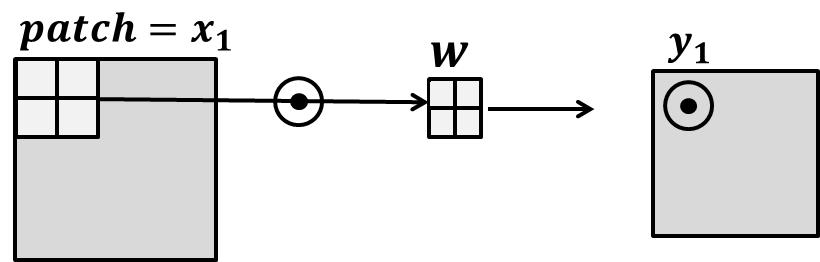
\includegraphics[height=3cm]{images/input_the_partial_convolution_graph.jpg}
            \caption{输入的部分卷积图}
            \label{fig:输入的部分卷积图}
            \end{figure}
            % \textcolor[rgb]{1 0 0}{todo:图片:输入的部分卷积图}\\
            % \textcolor[rgb]{1 0 0}{todo:加上原文中的fig1}\\
            我们将其展开,如图(\ref{fig:输入的部分卷积展开图})所示
            \begin{figure}[H]
            \centering
            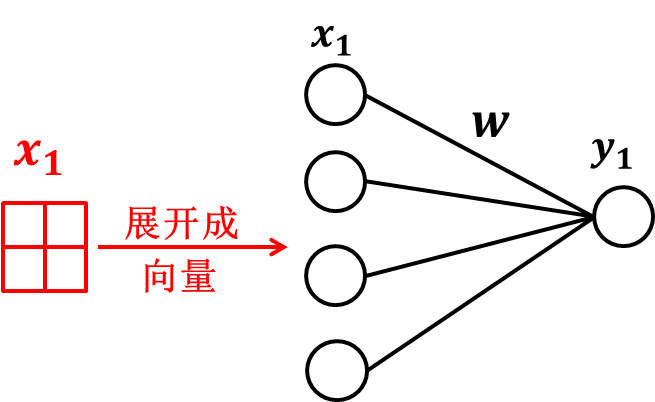
\includegraphics[height=3cm]{images/input_the_partial_convolution_unfold_graph.jpg}
            \caption{输入的部分卷积展开图}
            \label{fig:输入的部分卷积展开图}
            \end{figure}
            % \textcolor[rgb]{1 0 0}{todo:图片:输入的部分卷积展开图}\\
            图(\ref{fig:输入的部分卷积展开图})中有
            \begin{align*}
            y_1 = f(w^\mathrm{T}x_1)
            \end{align*}
            即输出图像的某一个像素点$y_1$就是原输入图像的部分$x_1$和卷积核$w$卷积而来(忽略$b$,不考虑多输入)。这是一个2层的MLP,我们考虑能否将这个2层的MLP加深?
            \par
            (2)mlpconv。malpconv的示意图如图(\ref{fig:mlpconv示意图})所示
            \begin{figure}[H]
                \centering
                \begin{subfigure}[b]{0.4\textwidth}
                    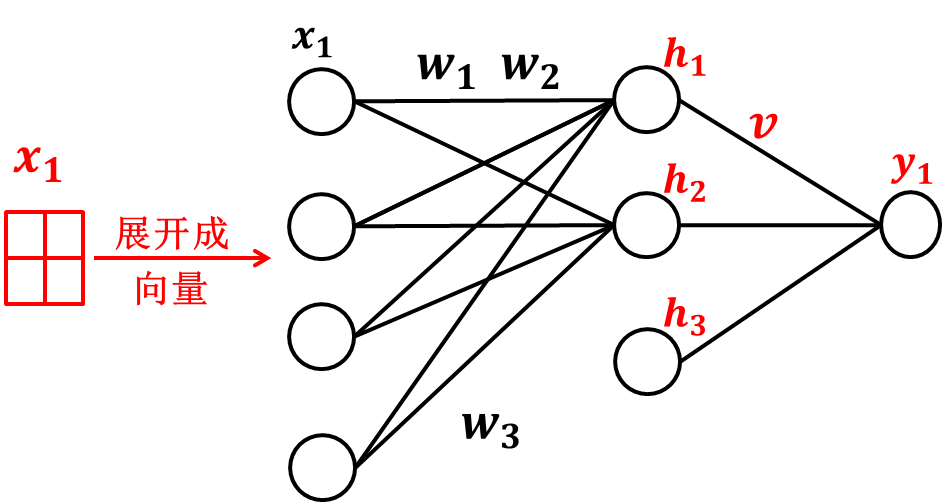
\includegraphics[width=\textwidth]{images/mlpconv1.jpg}
                    \caption{}
                    \label{fig:mlpconv示意图1}
                \end{subfigure}
                \begin{subfigure}[b]{0.4\textwidth}
                    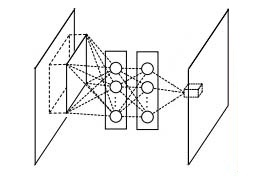
\includegraphics[width=\textwidth]{images/mlpconv2.jpg}
                    \caption{}
                    \label{fig:mlpconv示意图2}
                \end{subfigure}
                \caption{mlpconv示意图}\label{fig:mlpconv示意图}
            \end{figure}
            % \textcolor[rgb]{1 0 0}{todo:图片:mlpconv示意图(a)(b)}\\
            图(\ref{fig:mlpconv示意图1})中,令$w = (w_1,w_2,w_3)$我们有
            \begin{align*}
            & h_1 = f(w_1x_1)\\
            & h_2 = f(w_2x_1)\\
            & h_3=f(w_3x_1)\\
            & y=f_2(vh) = f_2(vf(w^\mathrm{T}x_1))
            \end{align*}
            前面只是用了一个卷积$w$,这里使用了3个卷积$w_1,w_2,w_3$就有3个输出,然后将它们汇聚在一起,就变成了一个3层的MLP。当然,可以继续加深网络。
            \par
            就整个输入矩阵$x$而言,我们设置了3个卷积核$w_1,w_2,w_3$,用这3个卷积核分别扫描$x$就有了3个输出,然后将其汇聚在一处,如图(\ref{fig:3个卷积核的mlpconv示意图})所示
             \begin{figure}[H]
            \centering
            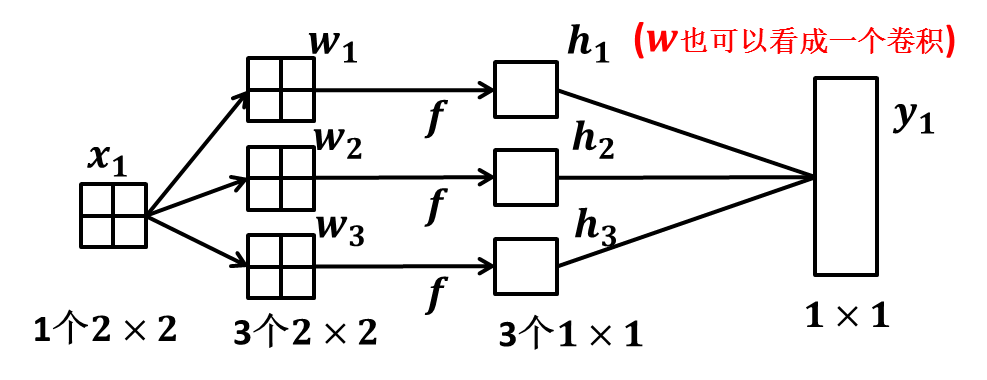
\includegraphics[height=3cm]{images/3convolution_mlpconv.jpg}
            \caption{3个卷积核的mlpconv示意图}
            \label{fig:3个卷积核的mlpconv示意图}
            \end{figure}
            % \textcolor[rgb]{1 0 0}{todo:图片:3个卷积核的mlpconv示意图}\\
            这里,也可以将$v$视为一个卷积核。有一个问题是:哪一层算作MLP的输入?为了将conv和mlp分开,将上面的$h_1,h_2,h_3$即卷积后面的输出作为mlp的输入。这样,上面的过程是一个1卷积conv加上2层mlp。将后面的mlp层加深,如图(\ref{fig:conv和3层mlp})所示
             \begin{figure}[H]
            \centering
            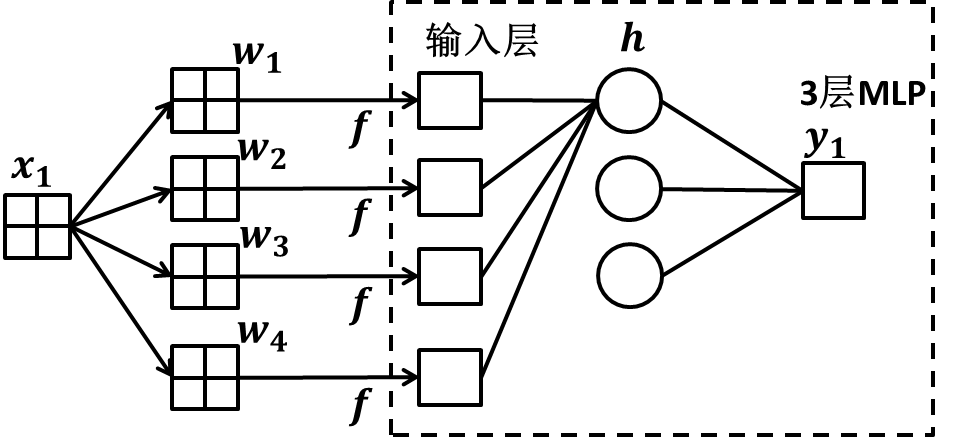
\includegraphics[height=3cm]{images/conv_and_3mlp.jpg}
            \caption{conv和3层mlp}
            \label{fig:conv和3层mlp}
            \end{figure}
            % \textcolor[rgb]{1 0 0}{todo:图片:conv和3层mlp}
            \par
            当然,上面两种理解都可以:$x$展开后直接mlp;$x$先卷积再mlp。二者本质上是一样的,并且注意,我们并不要mlp层数太多。
            \par
            (3)mlp = conv + $1\times 1$ conv。上面的分析只是对一个输入$x$而言,且$x$是一个矩阵(而RGB图像是一个张量)。对于单个输入$x$和单个卷积核$w$而言,$1\times 1$conv($1\times 1$卷积核)是易于理解的,卷积核的大小就是$1\times 1$。但实际上,CNN的卷积大多是多个maps和多个卷积核之间的操作。输入多个map和一组卷积核进行卷积操作,然后求和,得到一个输出map。如果此时使用$1\times 1$卷积核,其实就是\uline{多个feature map的线性组合}。
            \par
            文中提出了mlpconv其实等价于传统卷积核后接cccp层,从而实现多个feature map的线性组合,而cccp层与$1\times 1$卷积核是等价的。多输入的mlpconv(cccp层)如图(\ref{fig:cccp层示意图})所示
             \begin{figure}[H]
            \centering
            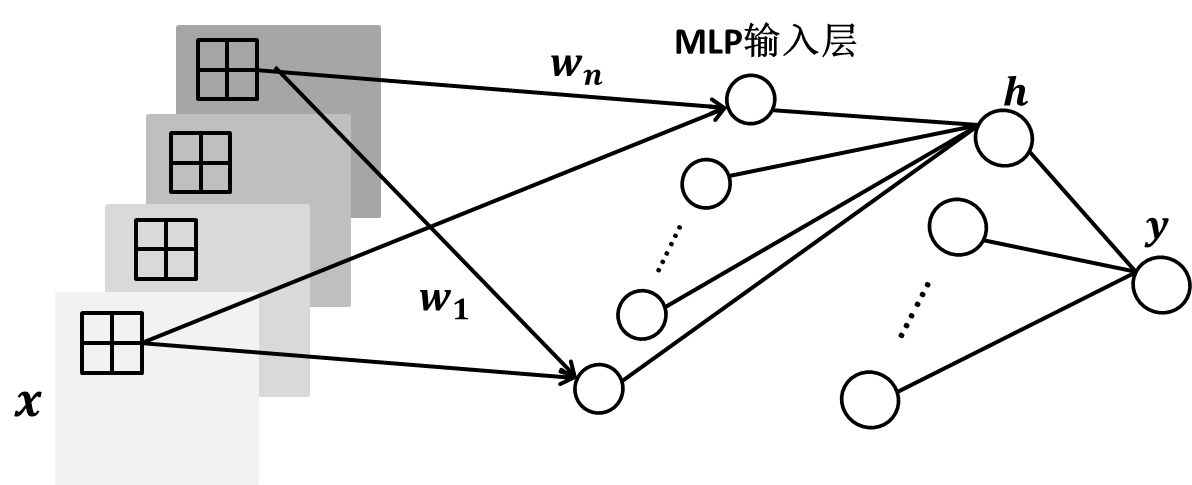
\includegraphics[height=3cm]{images/cccp_layer.jpg}
            \caption{cccp层示意图}
            \label{fig:cccp层示意图}
            \end{figure}
            % \textcolor[rgb]{1 0 0}{todo:图片:cccp层示意图}  \\
            如果要使MLP的输入有$n$个神经元,就需要$n$个卷积核$w_1,w_2,\dots,w_n$,从而实现上面的2个MLP。在caffe上的实现是:mlpconv = convenience + $1\times 1$conv + $1\times 1$conv。
        \subsubsection{Average Pooling}
            \par
            NiN\cite{2014.MinLin}中对CNN的第2处改进是使用全局平均pool来替代CNN中小分类器与卷积(池化)完全展开的接口。回忆一下CNN中的$S_4$到$F_5$层,是将$S_4$层的矩阵展开,然后拼接成$F_5$,如图(\ref{fig:CNN全展开层示意图})所示
             \begin{figure}[H]
            \centering
            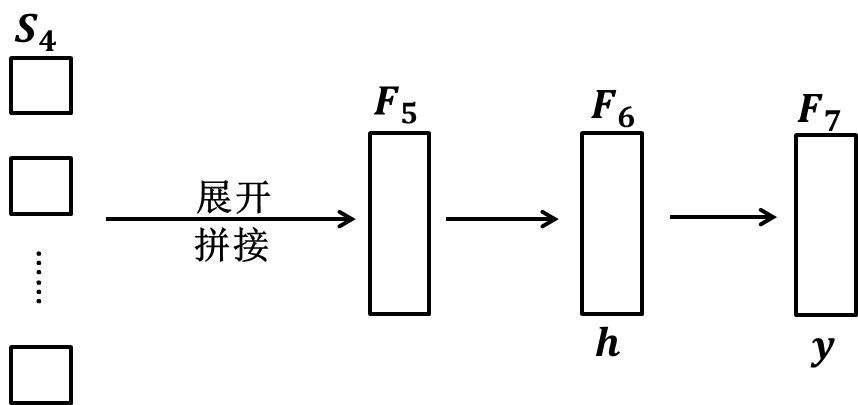
\includegraphics[height=3cm]{images/CNN_full_expanded_layer_diagram.jpg}
            \caption{CNN全展开层示意图}
            \label{fig:CNN全展开层示意图}
            \end{figure}
            % \textcolor[rgb]{1 0 0}{todo:图片:CNN全展开层示意图}\\
            然后,再将$F_5$层作为小分类器的输入层进行运行。但是,这样展开拼接有一个问题,就是展开之后的神经元输入太多了,导致小分类器的权重$w$矩阵是非常大的,不易求解。现在,我们将$S_4$的每个输出矩阵(feature map)求平均,然后再将平均值合并作为$F_5$层(小分类器的输入),如图(\ref{fig:average pooling示意图})所示
             \begin{figure}[H]
            \centering
            \includegraphics[height=3cm]{images/average_pooling.jpg}
            \caption{average pooling示意图}
            \label{fig:average pooling示意图}
            \end{figure}
            % \textcolor[rgb]{1 0 0}{todo:图片:average pooling示意图}\\
            这样,$S_4$层有几个矩阵,小分类器就有几个输入神经元。注:$S_4$到$F_5$的形式可以改进。
            \par
            称原本$S_4$到$F_5$为全连接;称改进后的$S_4$到$F_5$为Average pooling。
        \subsubsection{NiN的网络结构示意图}
            \par
            NiN网络结构示意图如图(\ref{fig:NiN网络结构示意图})所示
             \begin{figure}[H]
            \centering
            \includegraphics[height=3cm]{images/NiN_networks.jpg}
            \caption{NiN网络结构示意图}
            \label{fig:NiN网络结构示意图}
            \end{figure}
            % \textcolor[rgb]{1 0 0}{todo:图片:NiN网络结构示意图}
            \par
            基于TensorFlow实现的NiN网络如下\footnote{程序来自微信公众号:DLdigest 深度学习每日摘要(2017-05-09 )}
            \begin{lstlisting}[language = Python]
            import tensorflow as tfdef nin_cell(input):
                conv1_filter = tf.get_variable('conv1_filter', shape=[5, 5, 3, 192])
                conv1 = tf.nn.relu(tf.nn.conv2d(input, conv1_filter))
                mlpconv1_filter = tf.get_variable('mlpconv1_filter', shape=[1, 1, 192, 160])
                mlpconv1 = tf.nn.relu(tf.nn.conv2d(conv1, mlpconv1_filter))
                mlpconv2_filter = tf.get_variable('mlpconv2_filter', shape=[1, 1, 160, 96])
                mlpconv2 = tf.nn.relu(tf.nn.conv2d(mlpconv1, mlpconv2_filter))
                max_pool1 = tf.nn.max_pool(mlpconv2, ksize = [1,3,3,1], strides=[1,2,2,1])
                conv2_filter = tf.get_variable('conv2_filter', shape=[5, 5, 96, 192])
                conv2 = tf.nn.relu(tf.nn.conv2d(max_pool1, conv2_filter))
                mlpconv3_filter = tf.get_variable('mlpconv3_filter', shape=[1, 1, 192, 192])
                mlpconv3 = tf.nn.relu(tf.nn.conv2d(conv2, mlpconv3_filter))
                mlpconv4_filter = tf.get_variable('mlpconv4_filter', shape=[1, 1, 192, 192])
                mlpconv4 = tf.nn.relu(tf.nn.conv2d(mlpconv3, mlpconv4_filter))
                max_pool2 = tf.nn.max_pool(mlpconv4, ksize = [1,3,3,1], strides=[1,2,2,1])
                conv3_filter = tf.get_variable('conv3_filter', shape=[3, 3, 192, 192])
                conv3 = tf.nn.relu(tf.nn.conv2d(max_pool2, conv3_filter))
                mlpconv4_filter = tf.get_variable('mlpconv4_filter', shape=[1, 1, 192, 192])
                mlpconv4 = tf.nn.relu(tf.nn.conv2d(conv3, mlpconv4_filter))
                mlpconv5_filter = tf.get_variable('mlpconv5_filter', shape=[1, 1, 192, 10])
                mlpconv5 = tf.nn.relu(tf.nn.conv2d(mlpconv4, mlpconv5_filter))
                global_avg_pool = tf.nn.avg_pool(mlpconv5, ksize=[1,8,8,1])
                return global_avg_pool
            \end{lstlisting}
        \subsubsection{NiN的实验结果}
             \begin{figure}[H]
            \centering
            \includegraphics[width=10cm]{images/the_experimental_result_of_NiN_comparewith_other_networks_on_CIFAR-10_dataset.jpg}
            \caption{NiN与其它网络在CIFAR-10数据集上对比的实验结果
            }
            \end{figure}
            % \textcolor[rgb]{1 0 0}{todo:图片:NiN与其他网络在CIFAR-10数据集上对比的实验结果}


    \subsection{GoogLeNet}
        \subsubsection{GoogLeNet介绍}
            \par
            Szegedy等设计的GoogLeNet\cite{2014.Christian}在2014年的ILSVRC中获胜。它主要的贡献就是实现了一个奠基模块。它能够显著的减少网络中参数的数量,AlexNet中有6千万个,而它只有4万个。此外,GoogLeNet网络中没有使用卷积神经网络顶部的全连接层,而是使用了average pooling方法。ILSVRC2014年时采用的GoogLeNet有22层,参数比AlexNet少了12倍,但准确度更高(这说明AlexNet中还有许多不重要的参数,AlexNet还有很大的改进空间)。下面,我们来介绍GoogLeNet的2种重要的策略。
            \par
            (1)Motvation and High Level Considerations。直接提升深度卷积神经网络的方法是从深度和宽度两方面增加尺寸的,但是大的尺寸会使网络中有许多参数,容易出现过拟合现象,特别是当训练数据集不够大时。直接增加尺寸的另一个弊端是需要大量的计算资源。根本解决方法是将全连接层变为系数层。早些时候,为了打破网络的对称性和提高网络学习能力,传统网络使用了随机稀疏连接的方法。但是,非均匀系数网络的计算效率较低,我们可以将多个稀疏矩阵合并成相关的稠密子矩阵的方法来解决。
            \par
            (2)Incepion结构。Inception的主要思想是:怎样用密集成分来近似局部稀疏结构。GoogLeNet\cite{2014.Christian}中设计的Inception结构如图(\ref{fig:Inception结构示意图})所示
             \begin{figure}[H]
            \centering
            \includegraphics[height=3cm]{images/Inception_structure.jpg}
            \caption{Inception结构示意图}
            \label{fig:Inception结构示意图}
            \end{figure}
            % \textcolor[rgb]{1 0 0}{todo:图片:Inception结构示意图}
            \par
            我们采用大小不同的卷积对上一层的特征矩阵(例如:128个$100\times 100$的矩阵)进行卷积操作,提取不同维度的特征。这里卷积大小(1,3,5)不是必要的,可改。在卷积之后,将3个得到的卷积后的特征图/矩阵(maps)拼接起来(合并)。并且,为了使卷积后的maps的大小相同,在给定卷积步长$s=1$后,只要改变$pad=0,1,2$即可。由于pool层在许多实验中表现良好,所以也将其计算。但是$5\times 5$卷积核带来的计算量仍然是非常巨大的。为此,我们借鉴NiN的思路,用$1\times 1$卷积来降维,如图(\ref{fig:Inception结构cccp降维示意图})所示\\
             \begin{figure}[H]
            \centering
            \includegraphics[height=3cm]{images/Inception_structure_cccpDimensionality_reduction.jpg}
            \caption{Inception结构cccp降维示意图}
            \label{fig:Inception结构cccp降维示意图}
            \end{figure}
            % \textcolor[rgb]{1 0 0}{todo:图片:Inception结构cccp降维示意图}
            \par
            在$3\times 3$和$5\times 5$卷积前使用$1\times 1$卷积进行降维(将输入图片降维,例如:$256\to 64$)。这一层一般称为“瓶颈层”(bottleneck layer),\underline{它减小了每一层的特征map的数量},并由此减少了计算量。例如:假设我们输入层有256个特征图片,有256个输出,并且假定Inception层只进行$3\times 3$卷积操作,那么,它需要$256\times 256\times 3\times 3$(60万次)次卷积操作。如果用一个$1\times 1$的卷积核先将256卷积到64,然后再对64个特征图片进行$3\times 3$卷积操作,则有$64\times 64\times 3\times 3$卷积操作,然后,将64个输出maps再用$1\times 1$卷积返回,那么,这个操作为
            \begin{align*}
            256\times 1\times 1\times 64 + 64\times 64 \times 3\times 3 + 64\times 1\times 1\times 256 \approx 7\text{万}
            \end{align*}
            7万和60万相比,少了近10倍。鉴于GoogLeNet在图片问题上有良好的表现,下面来介绍4个改进版本。

        \subsubsection{GoogLeNet - V1}
            \par
            GoogLeNet\cite{2014.Christian}网络的核心就是Inception,其网络深度达到了27层。如此深的网络,它在BP反向传播过程中如何克服梯度消失问题呢?GoogLeNet用了一个先验信息:层数较小的网络也可能取得不错的分类效果。那么,深度网络中间层的特征对于分类来说,也是有很好的判别作用(即用中间特征做判别),所以,在中间的某些部分设置小的分类器来进行训练。训练阶段,总损失为总分类器和中间小分类器损失的和;在测试阶段,小分类器被弃用。GoogLeNet的网络结构如图(\ref{fig:GoogLeNet网络结构示意图})所示
             \begin{figure}[H]
            \centering
            \includegraphics[width=11cm]{images/GoogLeNet_steucture.jpg}
            \caption{GoogLeNet网络结构示意图}
            \label{fig:GoogLeNet网络结构示意图}
            \end{figure}
            % \textcolor[rgb]{1 0 0}{todo:图片:GoogLeNet网络结构示意图}\\
            GoogLeNet采用了模块组装的方式来搭建网络,这便于网络的添加和修改。并且,在网络的最后采用了average pooling来替代CNN的全连接。GoogLeNet中仍然采用了dropout策略,并在网络的中间层加了2个小分类器softmax,以避免梯度消失。小分类器的结构如图(\ref{fig:GoogLeNet小分类器的结构图})所示
             \begin{figure}[H]
            \centering
            \includegraphics[height=3cm]{images/The_structure_of_GoogLeNet_small_classifier.jpg}
            \caption{GoogLeNet小分类器的结构图}
            \label{fig:GoogLeNet小分类器的结构图}
            \end{figure}
            % \textcolor[rgb]{1 0 0}{todo:图片:GoogLeNet小分类器的结构图}\\
            average pooling部分的卷积核大小为$5\times 5$,步长$s >3$。
            % (4a)的输出为$4\times 4\times 512$,(4d)的输出为$4\times 4\times 518$,
            $1\times 1$的卷积核包含降维的$128$个卷积核和Relu,全连接层FC有1024个单元和修正线性激活,dropout层的dropped的输出比率为$20\%$,将softmax作为1000类的分类器的损失。
            \par
            GoogLeNet - V1最终top-5错误率在验证集和测试集上都是$6\%$,获得2014年的第一。GoogLeNet和其它网络的对比结果如图(\ref{fig:GoogLeNet在Top-5上的结果})所示
             \begin{figure}[H]
            \centering
            \includegraphics[height=3cm]{images/The_result_of_GoogLeNet_in_top5.jpg}
            \caption{GoogLeNet在Top-5上的结果}
            \label{fig:GoogLeNet在Top-5上的结果}
            \end{figure}
            % \textcolor[rgb]{1 0 0}{todo:图片:GoogLeNet在Top-5上的结果}

        \subsubsection{GoogLeNet - V2}
            \par
            2015.Sergey\cite{2015.Sergey}引入Batch-normalized Inception被视为Inception第二代。Batch-normalized 在一层的输出上计算所有特征映射的均值和方差,并用这些值规定它们的响应,这相当于数据增向(whiteniy),因此,使得所有神经图(nurmal maps)在同一范围有响应,而且是零均值,在下一层不需要从输入数据中学习offset时,这有助于训练。相关实现可以参考下面的网址\footnote{https://github.com/nutszebra/googlenet\_v2/blob/master/googlenet\_v2.py}。

        \subsubsection{GoogLeNet - V3}
            \par
            2015年12月,该团队发布了Inception-V3版本\cite{2015.Szegedy}。在Inception-V1时期,能与GoogLeNet能一较高下的只有VGG(这个下面介绍),但相比之下,GoogLeNet的计算效率要明显高于VGG。GoogLeNet表现虽然良好,但是,要想通过简单放大(大的卷积核)Inception结构来构建更大的网络则会立即增加消耗。
            \par
            大的卷积核可以带来更大的感知范围,但这也意味着我们将要训练更多的参数,比如$5\times 5$与$3\times 3$,二者的参数量为$25/9\approx 3$。为此,Sergey loffe等提出用2个连续的$3\times 3$卷积($s=1$)组成小网络来替代$5\times 5$。然而,这样有2个问题:\ding{172}这种替代会造成表达能力下降吗?即提取的特征会减少吗;\ding{173}$3\times 3$卷积之后,还要再激活吗?从大量的实验来看,表达能力不会下降,并且,增加非线性激活会提高性能,即$5\times 5$可以用2个$3\times 3$代替。那么,我们是否可以考虑更小的卷积核呢?比如$n\times 1$。
            \par
            于是,任意的$n\times n$卷积核都可以通过$1\times n$结合$n\times 1$来替代。作者发现,在网络前期使用这种替代效果并不好,如果在中等大小的feature map上使用效果要好一些(作者建议map大小在12到20之间)。于是,原GoogLeNet的inception变为图(\ref{fig:inception-v3示意图})(b)
            \begin{figure}[H]
              \centering
              \begin{varwidth}[t]{\textwidth}
                \vspace{0pt}
                \includegraphics[height=4cm]{images/inception_v3(a).jpg}
              \end{varwidth}
              \qquad\qquad
              \begin{varwidth}[t]{\textwidth}
                \vspace{0pt}
                \includegraphics[height=4cm]{images/inception_v3(b).jpg}
              \end{varwidth}
                        \caption{inception-v3示意图}
                        \label{fig:inception-v3示意图}
            \end{figure}
            % \textcolor[rgb]{1 0 0}{todo:图片:inception-v3示意图}\\
            图(\ref{fig:inception-v3示意图})(a)中用2个$3\times 3$来替代一个$5\times 5$,图(\ref{fig:inception-v3示意图})(b)中用$n\times 1$来替代$5\times 5$和$3\times 3$。当然,还可以将Inception设计为图(\ref{fig:inception-v3-2示意图})的形式。GoogLeNet - V3的实现可以参考\footnote{https://github.com/nutszebra/googlenet\_v3}
             \begin{figure}[H]
            \centering
            \includegraphics[height=3cm]{images/inception_v3_2.jpg}
            \caption{inception-v3-2示意图}
            \label{fig:inception-v3-2示意图}
            \end{figure}
            % \textcolor[rgb]{1 0 0}{todo;图片:inception-v3-2示意图}



        \subsubsection{GoogLeNet - V4}
            \par
            2016年8月,该团队再次更新了Inception的版本\cite{2016.Szegedy} :Inception-V4。Inception-V4中吸收了在2015ILSVRC中获胜的ResNet的特点,构建了Inception-ResNet模块。同时,文\cite{2016.Szegedy}中还发现,ResNet的结构可以极大的加速训练,同时性能也有提升,得到了一个Inception-ResNet-V2网络。此外,该团队还设计了一个更深更优化的Inception-V4模型,能够达到和Inception-ResNet-V2相似的性能。值得一提的是Inception-V4中没有Resdual操作。
            \par
            先来简单记一下Resdual操作,关于ResNet后面介绍。Resdual的经典结构如图(\ref{fig:Resdual结构示意图})所示
             \begin{figure}[H]
            \centering
            \includegraphics[height=3cm]{images/Resdual_structure.jpg}
            \caption{Resdual结构示意图}
            \label{fig:Resdual结构示意图}
            \end{figure}
            % \textcolor[rgb]{1 0 0}{todo:图片:Resdual结构示意图}\\
            我们将Inception和Resdual相结合,得到Inception-ResNet的经典模块如图(\ref{fig:Inception-ResNet-V1结构示意图})所示
             \begin{figure}[H]
            \centering
            \includegraphics[height=3cm]{images/Inception-ResNet-V1_structure.jpg}
            \caption{Inception-ResNet-V1结构示意图}
            \label{fig:Inception-ResNet-V1结构示意图}
            \end{figure}
            % \textcolor[rgb]{1 0 0}{todo:图片:Inception-ResNet-V1结构示意图}\\
            其余图片参考原文。网址\footnote{https://github.com/mtmd/GoogleNet\_MATLAB}给出了GoogleNet的MATLAB实现。

    \subsection{VGG Net}
        \par
        VGG是ILSVRC2014年比赛的第二名,仅次于GoogLeNet,由Karen Simanyan和Androw Izsserman 实现\cite{2014.KarenSzegedy}。它的主要贡献是展示出网络的深度是算法优良的关键。他们设计的最好的VGG网络包含16层,并且网络结构非常一致,统一使用$3\times 3$卷积层和$2\times 2$pooling层。但是VGG的计算量是非常大的,大量的参数导致它会占用很大的内存(140M),其中绝大多数参数都是来自于一个全连接层FC。后面,可以尝试将这个FC层去掉,以减少参数量。
        \par
        VGG同样是一种卷积神经网络,通常有16到19层,其网络结构如图(\ref{fig:VGG网络结构图})所示
             \begin{figure}[H]
            \centering
            \includegraphics[height=2cm]{images/VGG_Net_structure.jpg}
            \caption{VGG网络结构图}
            \label{fig:VGG网络结构图}
            \end{figure}
        % \textcolor[rgb]{1 0 0}{todo:图片:VGG网络结构图}
        \par
        注意,就像前面所说的那样,图(\ref{fig:VGG网络结构图})中的conv都是$3\times 3$大小,maxpool都是$2\times 2$大小。VGG正是试图通过多个$3\times 3$卷积来替代更大的卷积核(比如$5\times 5$ 和$7\times 7$),这也是前面Inception的策略。并且VGG-E第45块:$256\times 256$和$512\times 512$个$3\times 3$是卷积核依次使用多次,以提取到更多的特征maps以及这些maps的组合。其效果就等于是一个带有3个卷积层的大型$512\times 512$的大分类器,这意味着要有大量的参数。
        \par
        VGG实现细节:dropout只在前面2个FC中使用,在第3个FC中不用。使用批量为256的批量梯度算法SGD,同样采用动量权重更新,动量参数为0.9。VGG在目标中使用了L2正则项(惩罚项),罚权重为$5\time 10^{-4}$,dropout率为0.5,学习率初始值为$0.01$,并在validation error达到瓶颈之前以10倍下降,直到validation error不再变化。在实验中,学习率共降过3次,迭代次数有370千次,共74次对全部数据进行扫描。权重初始值使用Pre-traing(预训练)的方法:先预训练一小部分网络,当网络稳定后再向前训练。每次初始化权重时,使用$N(0,0.01)$,偏置$b$的初始值为0,传递函数使用Relu。

    \subsection{ResNet}
        \subsubsection{ResNet简介}
            \par
            ResNet\cite{2015.HeKaiming}是ILSVRC2015年的获胜者,由微软亚洲研究院的何凯明等研发,在图像分类、目标检测等任务中,ResNet的性能大幅度超越前一年的网络。残差网络的明显特征是有着相当深的网络深度,从32层到152层,深度远超之前的网络。并且,更有甚者设计了1001层的网络结构,其网络深度是令人吃惊的。残差网络使用了特殊的跳跃式连接,大量使用批量归一化(batch normalization),并且网络的最后也没有使用FC层。
            \par
            从前面介绍的CNN及其改进来看,似乎越深的网络表达能力越强。我们能不能将一个简单的网络加深,使它变得更优呢(不改变结构的情况下)?何凯明等人通过实验证明:在时间复杂度相同的情况下,深度较深的网络性能会更优一下,但是一般的堆积网络块并不能使网络更好。堆积的深层网络除了使计算量变大之外,另一大难题则是梯度消失(infernation),进而导致网络收敛缓慢。2013年,多伦多大学Lei jimny Ba和微软的RichCarnana发表了《Do Deepnets really need to be deep?》一文,文中用一个浅层网络去模拟一个深层网络,结果得到2个只有1层的浅层网络,但这个网络却能与深层网络相媲美。因此,作者提出,对浅层网络而言,可能还有许多更好的网络结构和更好的学习算法等待我们开发(这是重点)。同样,何凯明等在ResNet的原文\cite{2015.HeKaiming}中也做过实验,将网络的深度由20增加到56,发现随着网络深度的加深,错误率却不降反增,如图(\ref{fig:20vs56层(简单堆积加深)的结果图})所示
            \begin{figure}[H]
              \centering
              % \begin{varwidth}[t]{\textwidth}
              %   \vspace{0pt}
              %   \includegraphics[height=4cm]{images/20vs56layer_simple_stack1.jpg}
              % \end{varwidth}
              % \qquad
              % \begin{varwidth}[t]{\textwidth}
              %   \vspace{0pt}
                \includegraphics[height=4cm]{images/20vs56layer_simple_stack2.jpg}
              % \end{varwidth}
                \caption{20vs56层(简单堆积加深)的结果}
                \label{fig:20vs56层(简单堆积加深)的结果图}
            \end{figure}

% \begin{figure}[H]
%     \centering
%     \begin{subfigure}[b]{0.4\textwidth}
%         \includegraphics[width=\textwidth]{images/20vs56layer_simple_stack1.jpg}
%         \caption{}
%         \label{fig:20vs56层(简单堆积加深)的结果图1}
%     \end{subfigure}
%     \begin{subfigure}[b]{0.4\textwidth}
%         \includegraphics[width=\textwidth]{images/20vs56layer_simple_stack2.jpg}
%         \caption{}
%         \label{fig:20vs56层(简单堆积加深)的结果图2}
%     \end{subfigure}
%     \caption{20vs56层(简单堆积加深)的结果}
%     \label{fig:20vs56层(简单堆积加深)的结果图}
% \end{figure}
            % \textcolor[rgb]{1 0 0}{todo:图片:20vs56层(简单堆积加深)的结果图(a)(b)}
            从图(\ref{fig:20vs56层(简单堆积加深)的结果图})中可以看出,简单增加网络深度不仅仅使测试集错误率提高,而且在训练集中错误率也提高,这就排除了深度网络过拟合的可能(如果仅在测试集中错误率提高,则是网络过拟合)。模型中也使用了Relu和BN等防止梯度消失的策略,但最终结果表明:普通增加深度是有问题的,至于问题出在哪里,这个还有待研究。
        \subsubsection{高速公路网络HighWay Network}
            \par
            ResNet可以视为Highway network的特例。Highway Network\cite{2015.Rupesh}是瑞士3位学者于2015年提出的一种超深度的网络,为什么说是超深呢?原文\cite{2015.Rupesh}指出,他们能够训练900层的神经网络。虽然只是层数加深,没有性能的提高,但是能训练就已经很不错了。他们还在文中给出了最深达100层的Highway Net的收敛情况,如图(\ref{fig:HighWayNetwork的收敛情况})所示
             \begin{figure}[H]
            \centering
            \includegraphics[height=5cm]{images/HighWayNetwork_convergence.jpg}
            \caption{HighWayNetwork的收敛情况}
            \label{fig:HighWayNetwork的收敛情况}
            \end{figure}
            % \textcolor[rgb]{1 0 0}{todo;图片:HighWayNetwork的收敛情况}
            \par
            Highway Net的工作受到了LSTM(这个我们在RNN中介绍)中gate的启发:既然梯度在某些地方被阻碍了,那就让它直接通过这些阻碍层好了,不求导或者令导数为1。HighwayNet的思想正源于此,并且,这也是Highway名称的由来。在Highway网络中,我们设网络层数为$L$,$W_{H_l}(l=1,2,\dots,L)$表示第$l$层的权重,$H$为第$l$层的非线性函数,$x_1$是第1层的输入,$w_{H_1}$是第1层的权重,$y_1$是第1层的输出,忽略偏置$b$,并省略层$l$的标记,可以将输入输出写为
            \begin{align*}
            y = H(x,W_H)
            \end{align*}
            这里:$H$是一个仿射变换,但是,它还可以有更一般的形式,在Highway中,我们添加2个新的非线性转换$T(x,W_T),C(x,W_c)$,$y$为
            \begin{align*}
            y = H(x,W_H)T(x,W_T)+xC(x,W_c)
            \end{align*}
            我们定义$T$为转换门(transform gate),$C$是传递门(carry gate)。为了简单,令$C = 1-T$,于是有
            \begin{align*}
            y = H(x,W_H)T(x,W_T)+x[(1-T)(x,W_T)]
            \end{align*}
            由于是gate,所以$T$的取值为0或1。我们可以看到
            \begin{align*}
            y =
            \left\{
            \begin{aligned}
            x \qquad T = 0, \ \text{关闭}\\
            H(x,W_H)\qquad T = 1,\ \text{打开}
            \end{aligned}
            \right.
            \end{align*}
            这种思路是非常巧妙地,将上面的$y$关于$x$求导,有
            \begin{align*}
            \frac{\partial y}{\partial x} =
            \left\{
            \begin{aligned}
            I \quad T=0\\
            H'(x,W_H) \quad T=1
            \end{aligned}
            \right.
            \end{align*}
            其中:$I$是全1向量。上面的$y = x$代表着什么,想必也是了然的,这就是Highway。并且$\frac{\partial y}{\partial x} = I$也使梯度得以直接通过(很“变态”的一种方法)。使用TensorFlow实现HighwayNet如下\footnote{微信公众号:DLdigest深度学习每日摘要(2017-05-07)}
            \begin{lstlisting}[language = Python]
            def highwayUnit(input_layer, unit_id, is_training=True):
                with tf.variable_scope('HighwayUnit_'+str(unit_id), initializer=tf.random_normal_initializer()):
                    T = tf.layers.conv2d(input_layer, 32, (3,3), padding='same')
                    bn_layer1 = tf.contrib.layers.batch_norm(input_layer, is_training=is_training)
                    relu_layer1 = tf.nn.relu(bn_layer1)
                    conv_layer1 = tf.layers.conv2d(relu_layer1, 32, (3,3), padding='same')
                    bn_layer2 = tf.contrib.layers.batch_norm(conv_layer1, is_training=is_training)
                    relu_layer2 = tf.nn.relu(bn_layer2)
                    conv_layer2 = tf.layers.conv2d(relu_layer2, 32, (3,3), padding='same')
                return (1.0-T)*input_layer+T*conv_layer2
            \end{lstlisting}

        \subsubsection{ResNet理论}
            \par
            下面正式进入到ResNet中。像Highway那样,ResNet也使用了“直通”的方法,不过ResNet还采用了一些其他的技巧,从而使ResNet完全避免了梯度消失问题。
            \par
            我们知道,在一个浅层网络上累加/堆积一些$x_{l+1} = y = x_l$是不改变网络的结果的,它只是单纯的增加了网络的深度而已。但是,这样的“深”并非我们的初衷,我们希望加深网络来提高网络的性能。先来看一下一般的网络结构,如图(\ref{fig:一般的网络结构示意图})所示
             \begin{figure}[H]
            \centering
            \includegraphics[height=3cm]{images/normal_Network.jpg}
            \caption{一般的网络结构示意图}
            \label{fig:一般的网络结构示意图}
            \end{figure}
            % \textcolor[rgb]{1 0 0}{todo:图片:一般的网络结构示意图}\\
            要求经过两个权重层/卷积层后,输入的$x_{l+1} = x_l$。如果拟合/逼近一个恒等式$x_{l+1} = H(x_l)$不容易,可以转而拟合其误差,让其误差趋于0。并且由于要求$x_{l+1} = x_l$,所以二者的大小应该是一样的。拟合误差的网络如图(\ref{fig:误差块网络示意图})所示
             \begin{figure}[H]
            \centering
            \includegraphics[height=4cm]{images/Error_block_network_diagram.jpg}
            \caption{误差块网络示意图}
            \label{fig:误差块网络示意图}
            \end{figure}
            % \textcolor[rgb]{ 1 0 0}{todo:图片:误差块网络示意图}\\
            图(\ref{fig:误差块网络示意图})中,$F(x_l)$表示$x_{l+1}-x_l$。当$f(x) = x$时,为了方便,忽略层$l$的下标,有
            \begin{align*}
            & F(x) = W_2\sigma (W_1x)\\
            & y = x+F(x)\\
            & H(x_l) = f(y)
            \end{align*}
            \par
            我们写出更一般的残差块的公式,要求$x_l$到$x_{l+1}$为$h(x_l)$,有
            \begin{align*}
            & F(x) = W_2+\sigma(W_1x)\\
            & y = h(x)+F(x)\\
            & x_{l+1} = H(x_l) = f(y)
            \end{align*}
            其中:$x_l$是第$l$残差单元/残差块(residual unit)的输入特征maps(input feature maps);$W_l=\{W_{l,k|1 \leqslant k \leqslant K}\}$是第$l$层/残差块的权重,$W_l = (W_{l1},W_{l2})$。$K$是第$l$层的权重数量,或者说是第$l$个残差块的卷积层数;$F$是残差函数;$f$是传递函数,例如$f = Relu$;$h(x_l)$是$x_l$的一个变换,一般为恒等式$h(x_l) = x_l$。
            \par
            如果传递函数$f$也是一个恒等式,我们可以写出
            \begin{align*}
            x_{l+1} = x_l+F(x_l,W_l)
            \end{align*}
            将$L$个残差块堆积起来,则有
            \begin{align*}
            x_{l+2} = x_{l+1} + F(x_{l+1}, W_{l+1}) = x_l + F(x_l,W_l)+F(x_{l+1},W_{l+1})
            \end{align*}
            更一般的,有
            \begin{align*}
            x_L =x_l + \sum_{i=l}^{L-1}F(x_i,W_i)
            \end{align*}
            这里,为了便于理解,可以将$F(x_i,W_i)$视为0。对任何深度的$L$和任意的层/块$l$,上式有一些非常好的性质:
            \begin{enumerate}
            \item $\forall L$,特征$x_L$可以表示成$x_l(\forall l)$和$\sum\limits_{i=l}^{L-1}F(x_i,W_i)$的和;
            \item $\forall L$,$x_L =x_0 + \sum\limits_{i=0}^{L-1}F(x_i,W_i)$,即$x_L$是所有残差$F(x_i,W_i)$求和后加上$x_0$;
            \end{enumerate}
            \par
            记ResNet网络的最终误差为$E$,$E$关于$x_l$求导,有
            \begin{align*}
            \frac{\partial E}{\partial x_l} = \frac{\partial E}{\partial x_L} \frac{\partial x_L}{\partial x_l} = \frac{\partial E}{\partial x_L} \left( 1+\frac{\partial }{\partial x_l}\sum_{i=l}^{L-1}F(x_i,W_i) \right)
            \end{align*}
            上式表明,梯度$\frac{\partial E}{\partial x_l}$能够分解为2部分:$\frac{\partial E}{\partial x_L}$和$\frac{\partial E}{\partial x_L}\frac{\partial }{\partial x_l}\sum\limits_{i=l}^{L-1}F$。后面这部分$\frac{\partial E}{\partial x_L}$确保了信息/梯度可以传递到任何层$l$,并且保证了$\frac{\partial E}{\partial x_l}$不会消失。因为$\frac{\partial }{\partial x_l}\sum\limits_{i=l}^{L-1}F$对$x_l$不会总是$-1$,这里的梯度已经不再是一般的连乘$\frac{\partial }{\partial}\dots\frac{\partial }{\partial}$的形式了,所以不会消失。
            \par
            但是,要注意的是,前面假设了$h(x_l) = x_l$,并且假设$x_{l+1} =y_l$,这是两个非常强的约束,一旦打破,上述关系式即不成立。
            \par
            (1)对于第一个假设。关于$h(x_l) = x_l$是我们一直默认的,而且实验表明这种方法是较好的。现在,将其改为$h(x_l) = \lambda_l x_l$,并且仍然假设$x_{l+1} = y_l$(即传递函数$f$是恒等传递),有
            \begin{align*}
            x_{l+1} = \lambda_l x_l + F(x_l W_l)
            \end{align*}
            递归堆积,有
            \begin{align*}
            x_L = \prod_{i=l}^{L-1} \lambda_i x_l + \sum_{i=l}^{L-1}\prod_{j=i+1}^{L-1}\lambda_jF(x_i,W_i)
            \end{align*}
            或者简单记为
            \begin{align*}
            x_L = \prod_{i=l}^{L-1} \lambda_i x_l + \sum_{i=l}^{L-1}\hat{F}(x_i,W_i)
            \end{align*}
            其中:$\hat{F} = \prod\limits_{j=i+1}^{L-1}\lambda_jF(x_i,W_i)$。
            \par
            我们仍然记误差为$E$,$E$关于$x_l$求导,有
            \begin{align*}
            \frac{\partial E}{\partial x_l} = \frac{\partial E}{\partial x_L} \left( \prod_{i=l}^{L-1}\lambda_i + \frac{\partial }{\partial x_l} \sum_{i=l}^{L-1}\hat{F}(x_i,W_i) \right)
            \end{align*}
            第一项$\prod\limits_{i=l}^{L-1}\lambda_i $是非常危险的,如果对于所有的$i$,$\lambda_i >1$,那么这一项会按指数方式增长;如果对于所有的$i$,有$\lambda_i < 1$,那么这一项会减小甚至消失。因此,梯度很依赖$\lambda_i$而$\lambda_i$又不定,所以网络不稳定。
            \par
            (2)对于第二个假设。$x_{l+1} = f(y_l) = y_l$,将$f$放宽,不要求其为恒等变换,但是仍然要将$x_l$直接传递给$x_{l+1}$。为此,将$f$移到旁边的残差分支上来,至于$f\triangleq Relu$安放在哪里,可以参考何凯明文献\cite{2016.Kaiming}中的Fig4和Tab2,Fig4如图(\ref{fig:传递函数的6种不同的位置比较})所示,Tab2如图(\ref{fig:传递函数Tab2})所示
            \begin{figure}[H]
            \centering
            \includegraphics[width=12cm]{images/Transfer_func_of_six_different_location_compare.jpg}
            \caption{传递函数的6种不同的位置比较}
            \label{fig:传递函数的6种不同的位置比较}
            \end{figure}
            \begin{figure}[H]
            \centering
            \includegraphics[width=12cm]{images/Transfer_functab2.jpg}
            \caption{传递函数Tab2}
            \label{fig:传递函数Tab2}
            \end{figure}
            % \textcolor[rgb]{1 0 0}{todo:图片:传递函数的6种不同的位置}\\
            % \textcolor[rgb]{1 0 0}{todo:图片:传递函数Tab2}\\
            Fig4和Tab2中的比较表明:将$f=Relu$移到残差分支中,不仅可以满足之前的假设,而且是这几种移动中最优的移动。接下来使用TensorFlow来实现上图(\ref{fig:传递函数的6种不同的位置比较})所示的ResUnit
            \begin{lstlisting}[language = Python]
            import tensorflow as tf
            def resUnit(input_layer, unit_id, is_training=True):
                with tf.variable_scope('ResUnit_'+str(unit_id), initializer=tf.random_normal_initializer()):
                    bn_layer1 = tf.contrib.layers.batch_norm(input_layer, is_training=is_training)
                    relu_layer1 = tf.nn.relu(bn_layer1)
                    conv_layer1 = tf.layers.conv2d(relu_layer1, 32, (3,3), padding='same')
                    bn_layer2 = tf.contrib.layers.batch_norm(conv_layer1, is_training=is_training)
                    relu_layer2 = tf.nn.relu(bn_layer2)
                    conv_layer2 = tf.layers.conv2d(relu_layer2, 32, (3,3), padding='same')
                return input_layer+conv_layer2

            if __name__ == '__main__':
                with tf.Session() as sess:
                    input_layer = tf.get_variable('input', shape=[4,10,10,32], dtype=tf.float32)
                    out = resUnit(input_layer, 1)
                    sess.run(tf.global_variables_initializer())
                    print sess.run(out)
            \end{lstlisting}

            \par
            下面将残差块堆积起来,形成DeepResNet,如图(\ref{fig:DeepResNet网络结构图})所示
            \begin{figure}[H]
            \centering
            \includegraphics[height=12cm,angle=90]{images/DeepResNet_sructure.jpg}
            \caption{DeepResNet网络结构图}
            \label{fig:DeepResNet网络结构图}
            \end{figure}
            % \textcolor[rgb]{ 1 0 0}{todo:图片:DeepResNet网络结构图}
            \par
            ResNet层数逐步加深的训练误差如图(\ref{fig:ResNet层数逐步加深的训练误差})所示
            \begin{figure}[H]
            \centering
            \includegraphics[height=4cm]{images/trainingerror_of_The_number_of_ResNetlayers_gradually_deepen.jpg}
            \caption{ResNet层数逐步加深的训练误差}
            \label{fig:ResNet层数逐步加深的训练误差}
            \end{figure}
            % \textcolor[rgb]{1 0 0}{todo:图片:ResNet层数逐步加深的训练误差}
            从图(\ref{fig:ResNet层数逐步加深的训练误差})中可以看到,随着ResNet网络的加深,训练误差逐渐下降,没有出现普通堆积的误差增加的情况。
            \par
            下面,我们简记一下ResNet的结果。
            1. 2015年ResNet原文\cite{2015.HeKaiming}的Fig4和Tab2,在ImageNet数据集上进行了平整网络plain network和残差网络的收敛性对比;
            2. 2015年ResNet原文\cite{2015.HeKaiming}的Tab4,在ImageNet数据集上进行和ResNet与其它网络的的单一模型top-1和top-5的对比实验;
            3. 2015年ResNet原文\cite{2015.HeKaiming}的Tab5,在ImageNet数据集上进行和ResNet与其它网络的的集成模型top-5的对比实验;
            4. 2016年1001层残差网络的原文\cite{2016.Kaiming}的Fig3和Fig6,展示了1001层网络在CIFAR-10数据上的训练收敛图;
            5. 2016.Andreas在文\cite{2016.Andreas}中指出,ResNet其实质上并非一个非常深的网络,而是由指数个非常前的网络叠加而成。该论文同时指出,查看网络除了要看网络的深度和宽度(特征提取的多少)之外,还应该查看网络的multiplicity。重要观点查看原文Fig1即可。
            6. 2016.Zhang\cite{2016.Zhang}提出多级残差网络。网络结构参考原文\cite{2016.Zhang}的Fig1的RoR、Fig2的RoR-3和Fig3的Pre-RoR-3或RoR-3-WRN。
            7. 2016.Abdi\cite{2016.Abdi}同样提出多级残差网络。
            8. 2016.Zagoruyko\cite{2016.Zagoruyko}提出WResNet(WRN),将ResNet网络性能改善。
            9. 2016.Brian\cite{2016.Brian}对ResNet网络内部的特征进行了可视化。
            10. 2016.Gao\cite{2016.Gao}提出随机丢弃路径的网络。整个网络结构是随机的,并将该网络在CIFAR-10数据集上进行测试。
            11. 2016.Gustav\cite{2016.Gustav}提出了分形网络(fractal network)的概念,并在此基础上采用dropout方法进行训练。
    \subsection{MATLAB应用实例}
        \subsubsection{MATLAB自带CNN工具}
        \par
        MATLAB自带的卷积神经网络CNN命令如表(\ref{tab:CNN命令})所示
        \begin{table}[H]
          \caption{CNN命令}
          \label{tab:CNN命令}
          \centering
          \newcolumntype{Y}{>{\centering\arraybackslash}X}% 定义自适应列的居中格式 Y, 用 X 为左对齐(自适应列)
          \begin{tabularx}{\textwidth}{l|l}% 需要引入 tabularx 宏包;表格总宽度一定要设置
          \toprule
          命令  & 说明 \\
          \midrule
          trainingOptions &  Options for training neural network\\
          trainNetwork & Train a convolutional network\\
          imageInputLayer  & Image input layer\\
          convolution2dLayer & Convolutional layer\\
          reluLayer &  Rectified(改正) Linear Unit (ReLU) layer\\
          crossChannelNormalizationLayer&  Channel-wise local response normalization layer\\
          averagePooling2dLayer &  Average pooling layer object\\
          maxPooling2dLayer & Max pooling layer\\
          fullyConnectedLayer  & Fully connected layer\\
          dropoutLayer & Dropout layer\\
          softmaxLayer & Softmax layer for convolutional neural networks\\
          classificationLayer &  Create a classification output layer\\
          regressionLayer &  Create a regression output layer\\
          activations &  Compute convolutional neural network layer activations\\
          predict &  Predict responses using a trained convolutional neural network\\
          classify & Classify data using a trained convolutional neural network\\
          deepDreamImage&  Visualize(形象) network features using deep dream\\
          alexnet &  Pretrained AlexNet convolutional neural network\\
          vgg16  & Pretrained VGG-16 convolutional neural network\\
          vgg19 &  Pretrained VGG-19 convolutional neural network\\
          importCaffeLayers &  Import convolutional neural network layers from Caffe\\
          importCaffeNetwork & Import pretrained convolutional neural network models from Caffe\\
          SeriesNetwork &  Series network class\\
          TrainingOptionsSGDM &  Training options for stochastic gradient descent with momentum\\
          Layer&   Network layer\\
          ImageInputLayer&  Image input layer\\
          Convolution2DLayer & Convolutional layer\\
          ReLULayer &  Rectified(改正) Linear Unit (ReLU) layer\\
          CrossChannelNormalizationLayer&  Channel-wise local response normalization layer\\
          AveragePooling2DLayer &  Average pooling layer object\\
          MaxPooling2DLayer &  Max pooling layer\\
          FullyConnectedLayer &  Fully connected layer\\
          DropoutLayer & Dropout layer\\
          SoftmaxLayer & Softmax layer for convolutional neural networks\\
          ClassificationOutputLayer &  Classification output layer\\
          RegressionOutputLayer &  Regression output layer\\
          \bottomrule
          \end{tabularx}
        \end{table}

        \subsubsection{MatConvNet}
            \par
            MatConvNet是一个少有的基于MATLAB语言的深度学习工具箱,主要用于卷积神经网络(恰好就是我们这章所讲的内容)。MatConvNet包含了上面介绍的各大网络,并且由于上面的网络都比较大,MatConvNet在mat数据格式里已经提供了网络的基本结构,只需要将样本数据带入训练即可。
            MatConvNet基本模型示例:
            \begin{lstlisting}[language = Matlab]
            %% MatConvNet
            %1、 安装编译 MatConvNet (needed once).
            cnnMatFile = fullfile(matlabroot,'work','DL_song', 'MatConvNet');
            if ~exist(cnnMatFile, 'file') % download only once
                disp('Untar pre-trained CNN model...');
                MatConvNetPath = 'D:\Program Files\MATLAB\R2016a\work\深度学习\深度学习工具箱/matconvnet-1.0-beta23.tar.gz';
                untar(MatConvNetPath,cnnMatFile) ;
            end
            cnnMatFile = fullfile(cnnMatFile,'matconvnet-1.0-beta23');
            cd(cnnMatFile)
            % addpath matlab
            %编译
            run matlab/vl_compilenn ;%CPU编译
            %GPU编译
            vl_compilenn('enableGpu', true)
            %检测
            vl_testnn
            vl_testnn('gpu', true)
            %% VGG-face(人脸识别模型)
            % 下载已经训练好的模型 (needed once).注意:下载可能需要时间
            urlwrite(...
              'http://www.vlfeat.org/matconvnet/models/imagenet-vgg-f.mat', ...
              'imagenet-vgg-f.mat') ;
            % Setup MatConvNet.
            run matlab/vl_setupnn ;
            % Load a model and upgrade it to MatConvNet current version.
            net = load('imagenet-vgg-f.mat') ;
            net = vl_simplenn_tidy(net) ;
            % Obtain and preprocess an image.
            im = imread('peppers.png') ;
            im_ = single(im) ; % note: 255 range
            im_ = imresize(im_, net.meta.normalization.imageSize(1:2)) ;
            im_ = im_ - net.meta.normalization.averageImage ;
            % Run the CNN.
            res = vl_simplenn(net, im_) ;
            % Show the classification result.
            scores = squeeze(gather(res(end).x)) ;
            [bestScore, best] = max(scores) ;
            figure(1) ; clf ; imagesc(im) ;
            title(sprintf('%s (%d), score %.3f',...
               net.meta.classes.description{best}, best, bestScore)) ;
            %% DAG模型
            % setup MatConvNet
            run  matlab/vl_setupnn
            % 下载已经训练好的模型 (needed once)
            urlwrite(...
              'http://www.vlfeat.org/matconvnet/models/imagenet-googlenet-dag.mat', ...
              'imagenet-googlenet-dag.mat') ;
            % load the pre-trained CNN
            net = dagnn.DagNN.loadobj(load('imagenet-googlenet-dag.mat')) ;
            net.mode = 'test' ;
            % load and preprocess an image
            im = imread('peppers.png') ;
            im_ = single(im) ; % note: 0-255 range
            im_ = imresize(im_, net.meta.normalization.imageSize(1:2)) ;
            im_ = bsxfun(@minus, im_, net.meta.normalization.averageImage) ;
            % run the CNN
            net.eval({'data', im_}) ;
            % obtain the CNN otuput
            scores = net.vars(net.getVarIndex('prob')).value ;
            scores = squeeze(gather(scores)) ;
            % show the classification results
            [bestScore, best] = max(scores) ;
            figure(1) ; clf ; imagesc(im) ;
            title(sprintf('%s (%d), score %.3f',...
            net.meta.classes.description{best}, best, bestScore)) ;
            \end{lstlisting}
            \par
            我们还可以用MATLAB结合MatConvNet来建立网络,下面给出一个示例:
            \begin{lstlisting}[language = Matlab]
            %%%%%%%%%%%%%%%%%%%%%%%%%%%%%%%%%%%%%%%%%%%%%%%%%%%
            %% 这个例子展示深度学习模型CNN在图像识别中的应用
            %Note: 这个例子需要下面工具箱的支持:
            % Computer Vision System Toolbox?,
            % Image Processing Toolbox?,
            % Neural Network Toolbox?,
            % Parallel Computing Toolbox?,
            % Statistics and Machine Learning Toolbox?,
            % a CUDA-capable NVIDIA? GPU with compute capability 3.0 or higher.
            %%%%%%%%%%%%%%%%%%%%%%%%%%%%%%%%%%%%%%%%%%%%%%%%%%%
            %% 1、系统检验:为了检验你的计算机有一个CUDA-capable NVIDIA? GPU with compute capability 3.0 or higher.
            % 获得GPU设备的信息(GPU要求是NVIDIA的)
            deviceInfo = gpuDevice;
            % 检查GPU计算能力
            computeCapability = str2double(deviceInfo.ComputeCapability);
            assert(computeCapability > 3.0, ...
                'This example requires a GPU device with compute capability 3.0 or higher.')
            %% 2、下载图像数据
            % 从下面的网址下载压缩的数据
            url = 'http://www.vision.caltech.edu/Image_Datasets/Caltech101/101_ObjectCategories.tar.gz';
            % 将结果储存在一个临时文件夹
            outputFolder = fullfile(tempdir, 'caltech101'); %设置下载路径(图像数据下载在哪里)
            if ~exist(outputFolder, 'dir') %如果文件夹不存在,则下载并保存到该文件夹路径
                disp('Downloading 126MB Caltech101 data set...');
                untar(url, outputFolder);
            end
            %% 3、加载图像数据
            rootFolder = fullfile(outputFolder, '101_ObjectCategories');
            categories = {'airplanes', 'ferry', 'laptop'};%类别标签
            % 创建一个ImageDatastore来帮助您管理数据。因为ImageDatastore作用于图像文件位置,图像不加载到内存中,直到读,使其有效使用大型图像集合。
            imds = imageDatastore(fullfile(rootFolder, categories), 'LabelSource', 'foldernames');
            % imd变量现在包含图片和每个图像的分类标签。自动分配的标签图像文件的文件夹的名称。
            tbl = countEachLabel(imds)% 使用countEachLabel总结每个类别的图片数量。
            % 将3个类别中的图片数量取相同---67
            minSetCount = min(tbl{:,2}); %确定最小的类别数
            % 用splitEachLabel来随机选取图片,并使每个类别的图片大小为67
            imds = splitEachLabel(imds, minSetCount, 'randomize');%imds包含图片和类别
            % 再次展示个类别的数量
            countEachLabel(imds)
            % 找到每个类别的第一个图片
            airplanes = find(imds.Labels == 'airplanes', 1);
            ferry = find(imds.Labels == 'ferry', 1);
            laptop = find(imds.Labels == 'laptop', 1);
            % 将图片展示出来
            figure
            subplot(1,3,1);
            imshow(imds.Files{airplanes})
            subplot(1,3,2);
            imshow(imds.Files{ferry})
            subplot(1,3,3);
            imshow(imds.Files{laptop})
            %% 下载CNN模型(MatConvNet)
            % Location of pre-trained "AlexNet"
            cnnURL = 'http://www.vlfeat.org/matconvnet/models/beta16/imagenet-caffe-alex.mat';
            % Store CNN model in a temporary folder
            cnnMatFile = fullfile(tempdir, 'imagenet-caffe-alex.mat');
            if ~exist(cnnMatFile, 'file') % download only once
                disp('Downloading pre-trained CNN model...');
                websave(cnnMatFile, cnnURL);
            end
            %% 加载CNN模型
            % Load MatConvNet network into a SeriesNetwork
            convnet = helperImportMatConvNet(cnnMatFile)
            % 查看CNN结构
            convnet.Layers
            % 查看第一层网络
            convnet.Layers(1)
            % 查看最后一层网络
            convnet.Layers(end)
            % ImageNet分类任务类名称的数量
            numel(convnet.Layers(end).ClassNames)
            %% Pre-process Images For CNN
            % 如上所述,ConvNet的输入只能是RGB图像227-by-227。
            % Set the ImageDatastore ReadFcn
            imds.ReadFcn = @(filename)readAndPreprocessImage(filename);
            %% 设置训练集和测试集
            % 将集分为训练和验证数据。选择图像从每组训练数据的30%,其余70%,验证数据。
            % 随机分割来避免结果的偏差。训练集和测试集将由CNN模型处理。
            [trainingSet, testSet] = splitEachLabel(imds, 0.3, 'randomize');
            %% 观察中间层提取的特征
            % 得到第二卷积层的网络权重
            w1 = convnet.Layers(2).Weights;
            % Scale and resize the weights for visualization
            w1 = mat2gray(w1);
            w1 = imresize(w1,5);
            % Display a 混合图 of network weights. There are 96 个体 sets of
            % weights in the first layer.
            figure
            montage(w1)
            title('First convolutional layer weights')
            % 注意网络的第一层已经学会过滤器捕捉blob和边缘特征。
            % 这些“原始”功能被更深的网络层处理,并结合早期功能形成更高层次的图像特征。
            % 这些更高层次特性更适合识别任务,因为他们将所有的原始功能合并到更丰富的图像表示
            % You can easily extract features from one of the deeper layers using the activations method.
            % Selecting which of the deep layers to choose is a design choice,
            % but typically starting with the layer right before the classification layer is a good place to start.
            % In convnet, the this layer is named 'fc7'.
            Let's extract training features using that layer.
            featureLayer = 'fc7';
            trainingFeatures = activations(convnet, trainingSet, featureLayer, ...
                'MiniBatchSize', 32, 'OutputAs', 'columns');
            % 注意,激活计算GPU和“MiniBatchSize”设置32确保CNN和图像数据适合GPU内存。
            % 你可能需要降低“MiniBatchSize”如果你的GPU耗尽内存。
            % 此外,激活输出安排列。这有助于加速多级线性支持向量机训练。
            %% Train A Multiclass SVM Classifier Using CNN Features
            % Get training labels from the trainingSet
            trainingLabels = trainingSet.Labels;
            % Train multiclass SVM classifier using a fast linear solver, and set
            % 'ObservationsIn' to 'columns' to match the arrangement used for training
            % features.
            classifier = fitcecoc(trainingFeatures, trainingLabels, ...
                'Learners', 'Linear', 'Coding', 'onevsall', 'ObservationsIn', 'columns');
            %% 评估分类器
            % Extract test features using the CNN
            testFeatures = activations(convnet, testSet, featureLayer, 'MiniBatchSize',32);
            % Pass CNN image features to trained classifier
            predictedLabels = predict(classifier, testFeatures);
            % Get the known labels
            testLabels = testSet.Labels;
            % Tabulate the results using a confusion matrix.
            confMat = confusionmat(testLabels, predictedLabels);
            % Convert confusion matrix into percentage form
            confMat = bsxfun(@rdivide,confMat,sum(confMat,2))
            % Display the mean accuracy
            mean(diag(confMat))
            %% 对新图像进行分类
            newImage = fullfile(rootFolder, 'airplanes', 'image_0690.jpg');
            % Pre-process the images as required for the CNN
            img = readAndPreprocessImage(newImage);
            % Extract image features using the CNN
            imageFeatures = activations(convnet, img, featureLayer);
            % Make a prediction using the classifier
            label = predict(classifier, imageFeatures)
            \end{lstlisting}

\section{循环神经网络RNN}
% \section{对抗生成网络GAN}

% \bibliography{part-MLDL-chap-DeepLearn}%bib文件名称
% \end{document}
    todo:这是很有必要补充的一章!!!\footnote{稿子已经有了,我们正在想要不要添加进来。。。}
